% Options for packages loaded elsewhere
\PassOptionsToPackage{unicode}{hyperref}
\PassOptionsToPackage{hyphens}{url}
\documentclass[
  english,
]{article}
\usepackage{xcolor}
\usepackage{amsmath,amssymb}
\setcounter{secnumdepth}{5}
\usepackage{iftex}
\ifPDFTeX
  \usepackage[T1]{fontenc}
  \usepackage[utf8]{inputenc}
  \usepackage{textcomp} % provide euro and other symbols
\else % if luatex or xetex
  \usepackage{unicode-math} % this also loads fontspec
  \defaultfontfeatures{Scale=MatchLowercase}
  \defaultfontfeatures[\rmfamily]{Ligatures=TeX,Scale=1}
\fi
% \usepackage{lmodern}
\ifPDFTeX\else
  % xetex/luatex font selection
\fi
% Use upquote if available, for straight quotes in verbatim environments
\IfFileExists{upquote.sty}{\usepackage{upquote}}{}
\IfFileExists{microtype.sty}{% use microtype if available
  \usepackage[]{microtype}
  \UseMicrotypeSet[protrusion]{basicmath} % disable protrusion for tt fonts
}{}
\makeatletter
\@ifundefined{KOMAClassName}{% if non-KOMA class
  \IfFileExists{parskip.sty}{%
    \usepackage{parskip}
  }{% else
    \setlength{\parindent}{0pt}
    \setlength{\parskip}{6pt plus 2pt minus 1pt}}
}{% if KOMA class
  \KOMAoptions{parskip=half}}
\makeatother
\usepackage{color}
\usepackage{fancyvrb}
\newcommand{\VerbBar}{|}
\newcommand{\VERB}{\Verb[commandchars=\\\{\}]}
\DefineVerbatimEnvironment{Highlighting}{Verbatim}{commandchars=\\\{\}}
% Add ',fontsize=\small' for more characters per line
\newenvironment{Shaded}{}{}
\newcommand{\AlertTok}[1]{\textcolor[rgb]{1.00,0.00,0.00}{\textbf{#1}}}
\newcommand{\AnnotationTok}[1]{\textcolor[rgb]{0.38,0.63,0.69}{\textbf{\textit{#1}}}}
\newcommand{\AttributeTok}[1]{\textcolor[rgb]{0.49,0.56,0.16}{#1}}
\newcommand{\BaseNTok}[1]{\textcolor[rgb]{0.25,0.63,0.44}{#1}}
\newcommand{\BuiltInTok}[1]{\textcolor[rgb]{0.00,0.50,0.00}{#1}}
\newcommand{\CharTok}[1]{\textcolor[rgb]{0.25,0.44,0.63}{#1}}
\newcommand{\CommentTok}[1]{\textcolor[rgb]{0.38,0.63,0.69}{\textit{#1}}}
\newcommand{\CommentVarTok}[1]{\textcolor[rgb]{0.38,0.63,0.69}{\textbf{\textit{#1}}}}
\newcommand{\ConstantTok}[1]{\textcolor[rgb]{0.53,0.00,0.00}{#1}}
\newcommand{\ControlFlowTok}[1]{\textcolor[rgb]{0.00,0.44,0.13}{\textbf{#1}}}
\newcommand{\DataTypeTok}[1]{\textcolor[rgb]{0.56,0.13,0.00}{#1}}
\newcommand{\DecValTok}[1]{\textcolor[rgb]{0.25,0.63,0.44}{#1}}
\newcommand{\DocumentationTok}[1]{\textcolor[rgb]{0.73,0.13,0.13}{\textit{#1}}}
\newcommand{\ErrorTok}[1]{\textcolor[rgb]{1.00,0.00,0.00}{\textbf{#1}}}
\newcommand{\ExtensionTok}[1]{#1}
\newcommand{\FloatTok}[1]{\textcolor[rgb]{0.25,0.63,0.44}{#1}}
\newcommand{\FunctionTok}[1]{\textcolor[rgb]{0.02,0.16,0.49}{#1}}
\newcommand{\ImportTok}[1]{\textcolor[rgb]{0.00,0.50,0.00}{\textbf{#1}}}
\newcommand{\InformationTok}[1]{\textcolor[rgb]{0.38,0.63,0.69}{\textbf{\textit{#1}}}}
\newcommand{\KeywordTok}[1]{\textcolor[rgb]{0.00,0.44,0.13}{\textbf{#1}}}
\newcommand{\NormalTok}[1]{#1}
\newcommand{\OperatorTok}[1]{\textcolor[rgb]{0.40,0.40,0.40}{#1}}
\newcommand{\OtherTok}[1]{\textcolor[rgb]{0.00,0.44,0.13}{#1}}
\newcommand{\PreprocessorTok}[1]{\textcolor[rgb]{0.74,0.48,0.00}{#1}}
\newcommand{\RegionMarkerTok}[1]{#1}
\newcommand{\SpecialCharTok}[1]{\textcolor[rgb]{0.25,0.44,0.63}{#1}}
\newcommand{\SpecialStringTok}[1]{\textcolor[rgb]{0.73,0.40,0.53}{#1}}
\newcommand{\StringTok}[1]{\textcolor[rgb]{0.25,0.44,0.63}{#1}}
\newcommand{\VariableTok}[1]{\textcolor[rgb]{0.10,0.09,0.49}{#1}}
\newcommand{\VerbatimStringTok}[1]{\textcolor[rgb]{0.25,0.44,0.63}{#1}}
\newcommand{\WarningTok}[1]{\textcolor[rgb]{0.38,0.63,0.69}{\textbf{\textit{#1}}}}
\usepackage{longtable,booktabs,array}
\usepackage{caption}
\captionsetup[table]{skip=6pt}
\newcounter{none} % for unnumbered tables
\usepackage{calc} % for calculating minipage widths
% Correct order of tables after \paragraph or \subparagraph
\usepackage{etoolbox}
\makeatletter
\patchcmd\longtable{\par}{\if@noskipsec\mbox{}\fi\par}{}{}
\makeatother
% Allow footnotes in longtable head/foot
\IfFileExists{footnotehyper.sty}{\usepackage{footnotehyper}}{\usepackage{footnote}}
\makesavenoteenv{longtable}
\usepackage{graphicx}
\makeatletter
\newsavebox\pandoc@box
\newcommand*\pandocbounded[1]{% scales image to fit in text height/width
  \sbox\pandoc@box{#1}%
  \Gscale@div\@tempa{\textheight}{\dimexpr\ht\pandoc@box+\dp\pandoc@box\relax}%
  \Gscale@div\@tempb{\linewidth}{\wd\pandoc@box}%
  \ifdim\@tempb\p@<\@tempa\p@\let\@tempa\@tempb\fi% select the smaller of both
  \ifdim\@tempa\p@<\p@\scalebox{\@tempa}{\usebox\pandoc@box}%
  \else\usebox{\pandoc@box}%
  \fi%
}
% Set default figure placement to htbp
\def\fps@figure{htbp}
\makeatother
\ifLuaTeX
\usepackage[bidi=basic,shorthands=off]{babel}
\else
\usepackage[bidi=default,shorthands=off]{babel}
\fi
\ifLuaTeX
  \usepackage{selnolig} % disable illegal ligatures
\fi
\setlength{\emergencystretch}{3em} % prevent overfull lines
\providecommand{\tightlist}{%
  \setlength{\itemsep}{0pt}\setlength{\parskip}{0pt}}
\usepackage[]{natbib}
\bibliographystyle{plainnat}
\makeatletter
\@ifpackageloaded{subcaption}{}{\usepackage{subcaption}}
\@ifpackageloaded{caption}{}{\usepackage{caption}}
\captionsetup[subfigure]{margin=0.5em}
\AtBeginDocument{%
\renewcommand*\figurename{Figure}
\renewcommand*\tablename{Table}
}
\AtBeginDocument{%
\renewcommand*\listfigurename{List of Figures}
\renewcommand*\listtablename{List of Tables}
}
\newcounter{pandoccrossref@subfigures@footnote@counter}
\newenvironment{pandoccrossrefsubfigures}{%
\setcounter{pandoccrossref@subfigures@footnote@counter}{0}
\begin{figure}\centering%
\gdef\global@pandoccrossref@subfigures@footnotes{}%
\DeclareRobustCommand{\footnote}[1]{\footnotemark%
\stepcounter{pandoccrossref@subfigures@footnote@counter}%
\ifx\global@pandoccrossref@subfigures@footnotes\empty%
\gdef\global@pandoccrossref@subfigures@footnotes{{##1}}%
\else%
\g@addto@macro\global@pandoccrossref@subfigures@footnotes{, {##1}}%
\fi}}%
{\end{figure}%
\addtocounter{footnote}{-\value{pandoccrossref@subfigures@footnote@counter}}
\@for\f:=\global@pandoccrossref@subfigures@footnotes\do{\stepcounter{footnote}\footnotetext{\f}}%
\gdef\global@pandoccrossref@subfigures@footnotes{}}
\@ifpackageloaded{float}{}{\usepackage{float}}
\floatstyle{ruled}
\@ifundefined{c@chapter}{\newfloat{codelisting}{h}{lop}}{\newfloat{codelisting}{h}{lop}[chapter]}
\floatname{codelisting}{Listing}
\newcommand*\listoflistings{\listof{codelisting}{List of Listings}}
\makeatother
\usepackage{bookmark}
\IfFileExists{xurl.sty}{\usepackage{xurl}}{} % add URL line breaks if available
\urlstyle{same}
% fallback for those not using the hyperref driver hyperxmp:
\makeatletter
\@ifundefined{xmpquote}{\newcommand{\xmpquote}[1]{#1}}{}
\makeatother
\hypersetup{
  pdftitle={Active Skillference: A Provenance-Bound Curriculum and Reproducible Learning Infrastructure for Active Inference},
  pdfauthor={Daniel Ari Friedman},
  pdflang={en},
  colorlinks=true,linkcolor=red,urlcolor=red,citecolor=red,anchorcolor=red,filecolor=red,
  pdfcreator={LaTeX via pandoc}}

\title{Active Skillference: A Provenance-Bound Curriculum and
Reproducible Learning Infrastructure for Active Inference}
\author{Daniel Ari Friedman}
\date{}

\IfFileExists{seqsplit.sty}{\usepackage{seqsplit}}{\newcommand{\seqsplit}[1]{#1}}
\protected\def\breakseq#1{\seqsplit{#1}}
\protected\def\breaktt#1{\begingroup\ttfamily\seqsplit{#1}\endgroup}
\title{Active Skillference}
\author{Daniel Ari Friedman\\\footnotesize{Active Inference Institute}\\\footnotesize{\texttt{daniel@activeinference.institute}}\\\footnotesize{\href{https://orcid.org/0000-0001-6232-9096}{ORCID: 0000-0001-6232-9096}} \\ \footnotesize{DOI: \href{https://doi.org/10.5281/zenodo.21865644}{10.5281/zenodo.21865644}}}
\date{2026}

% Core mathematics
\usepackage{amsmath}
\usepackage{amssymb}
\usepackage{amsfonts}
\usepackage{amsthm}
% The renderer may use these environments for structured remarks/examples even when
% the source manuscript contains none. Define the counter they share explicitly so
% Pandoc's injected declarations cannot reference an undefined theorem counter.
\newtheorem{theorem}{Theorem}
\newtheorem{remark}[theorem]{Remark}
\newtheorem{example}[theorem]{Example}

% Document layout
\usepackage{geometry}
% Keep the requested near-edge-to-edge horizontal layout while preserving a modest
% vertical breathing room for headers, footers, and page-turn readability.
\geometry{left=0.10in,right=0.10in,top=0.25in,bottom=0.25in}
\usepackage{float}
\usepackage{graphicx}

% Tables
\usepackage{booktabs}
\usepackage{longtable}
\usepackage{array}

% Algorithm typesetting (for pseudocode in §2 Methodology)
\usepackage[ruled,vlined,linesnumbered]{algorithm2e}

% Code listings
\usepackage{listings}

% Typography and formatting
\usepackage{microtype}
\usepackage{xcolor}
\usepackage{siunitx}

% Cross-references and citations
\usepackage{hyperref}
\hypersetup{
    colorlinks=true,
    allcolors=red
}
\usepackage[capitalise,noabbrev]{cleveref}
\usepackage{natbib}

% ── Unicode-capable mono font for code listings ──────────────────────
% JuliaMono (TeX Live 2026) covers the full math/Greek glyph set used in
% scientific code blocks; the default lmmono lacks \alpha/\mu/\partial/\nabla.
%
% Prefer the pinned TeX Live font when present, but keep the manuscript compilable
% on TeX Live versions or distributions that install a different mono font set.
\usepackage{fontspec}
\IfFileExists{/usr/local/texlive/2026/texmf-dist/fonts/truetype/public/juliamono/JuliaMono-Regular.ttf}{%
  \setmonofont{JuliaMono-Regular}[
    Path           = /usr/local/texlive/2026/texmf-dist/fonts/truetype/public/juliamono/,
    Extension      = .ttf,
    UprightFont    = *,
    BoldFont       = JuliaMono-Bold,
    ItalicFont     = JuliaMono-RegularItalic,
    BoldItalicFont = JuliaMono-BoldItalic,
    Scale          = MatchLowercase,
  ]%
}{%
  \setmonofont{Latin Modern Mono}%
}

% Math font for unicode-math: Latin Modern Math (TeX Live) has full BMP
% coverage including U+2223 (\mid), U+226A/226B (\ll/\gg), and the Greek/
% blackboard letters used in equations. Without an explicit \setmathfont,
% unicode-math falls back to lmroman text font which lacks several glyphs
% and emits "Missing character" warnings on every \mid in math mode.
\setmathfont{latinmodern-math.otf}

\begin{document}
\begin{titlepage}
\thispagestyle{empty}
\setcounter{page}{1}
\centering
\vspace*{0.6cm}
{\Huge\sffamily\bfseries Active Skillference\par}
\vspace{0.35cm}
{\Large\sffamily A Validated Prerequisite Graph, Computational Claim Registry, and SkillTree Delivery Contract\par}
\vspace{0.8cm}
{\Large\bfseries Daniel Ari Friedman}\\[0.35em]
{\normalsize Active Inference Institute}\\[0.25em]
{\normalsize\texttt{daniel@activeinference.institute}}\\[0.25em]
{\normalsize\href{https://orcid.org/0000-0001-6232-9096}{ORCID: 0000-0001-6232-9096}}\\[0.5em]
\vfill
\includegraphics[width=0.98\textwidth,height=0.62\textheight,keepaspectratio]{\detokenize{../figures/active_skillference_cover.png}}
\vfill
{\small Edition 1.0.1 -- 2026}
{\small DOI: \href{https://doi.org/10.5281/zenodo.21865644}{10.5281/zenodo.21865644}\par}
\end{titlepage}
\clearpage
\thispagestyle{empty}
\section*{Publishing Information}

\noindent{\Large\bfseries Active Skillference}\\
{\large A Validated Prerequisite Graph, Computational Claim Registry, and SkillTree Delivery Contract}\\[1.2em]
{\Large\bfseries Daniel Ari Friedman}\\[0.35em]
{\normalsize Active Inference Institute}\\[0.25em]
{\normalsize\texttt{daniel@activeinference.institute}}\\[0.25em]
{\normalsize\href{https://orcid.org/0000-0001-6232-9096}{ORCID: 0000-0001-6232-9096}}\\[0.5em]
\vspace{1.0em}
\noindent Edition 1.0.1 -- 2026\\
\noindent Text license: MIT\\
\noindent Source-code license: MIT\\
\noindent DOI: \href{https://doi.org/10.5281/zenodo.21865644}{10.5281/zenodo.21865644}\\
\noindent Source repository: \href{https://github.com/ActiveInferenceInstitute/Active_Skillference}{https://github.com/ActiveInferenceInstitute/Active\_Skillference}\\
\vspace{0.8em}
\begin{center}
{\sffamily\bfseries Named Skill Atlas\par}
\vspace{0.35em}
\includegraphics[width=0.94\textwidth,height=0.50\textheight,keepaspectratio]{\detokenize{../figures/active_skillference_skill_atlas.png}}
\par\vspace{0.35em}
\begin{minipage}{0.92\textwidth}
{\scriptsize All exported skill names are tokenized into a deterministic front-matter atlas; visible labels are readable representatives rather than a complete printed index.}
\end{minipage}
\end{center}
\vspace{1.0em}
\noindent Suggested citation: Daniel Ari Friedman (2026). \textit{Active Skillference: A Validated Prerequisite Graph, Computational Claim Registry, and SkillTree Delivery Contract} (Edition 1.0.1). Active Inference Institute. \href{https://github.com/ActiveInferenceInstitute/Active_Skillference}{https://github.com/ActiveInferenceInstitute/Active\_Skillference}. \href{https://doi.org/10.5281/zenodo.21865644}{https://doi.org/10.5281/zenodo.21865644}.

\vspace{1.0em}
\noindent This open textbook is generated from version-controlled Markdown, tested Python modules, programmatic figures, and rendered Mermaid diagrams. Corrections and improvements may be submitted via the source repository linked above.

\vfill
\noindent Accessibility note: the compact PDF is optimized for dense print. Reader-profile builds, HTML output, and source Markdown can be generated from the same manuscript materials.
\clearpage
\tableofcontents
\clearpage

\section{Abstract: Active Skillference as Provenance-Bound Curriculum
Infrastructure}\label{abstract-active-skillference-as-provenance-bound-curriculum-infrastructure}

Active Inference and the Free Energy Principle (FEP) provide model-based
accounts of belief updating, learning, and action under uncertainty. We
present Active Skillference, a provenance-bound curriculum-generation
and SkillTree-export system for teaching those formal ideas. The paper
evaluates structural validity, quantitative provenance, citation-role
coverage, and artifact reproducibility; it does not evaluate learner
outcomes, establish a new theory of Active Inference, or present an
intelligent tutoring system.

The curriculum is expressed as code: a typed, validated directed acyclic
graph of 630 skills across 111 subjects spanning all 8 strata
(mathematics -\textgreater{} probability -\textgreater{} information
theory -\textgreater{} variational methods -\textgreater{} the FEP
-\textgreater{} active inference -\textgreater{} computation
-\textgreater{} applications), connected by 1199 prerequisite edges with
a maximum dependency depth of 75 (of which the substantive concept chain
accounts for 33; the remaining depth is per-stratum review and mastery
sequencing rather than conceptual prerequisite, as the methodology
details). Its defining feature is content-provenance binding: every
quantitative value shown to a learner is produced by a tested
computational kernel and inserted through a typed claim token, never
hand-typed, and the build refuses to export if a claim is unbacked or if
a bare result number appears in learner prose, manuscript prose, or
correct numeric quiz answers. The contribution is therefore a systems
and curriculum-infrastructure artifact: it makes a formal subject
inspectable and deliverable, but does not claim that the resulting path
is optimal for every learner.

The validated graph exports directly into SkillTree's data model
(Project -\textgreater{} Subjects -\textgreater{} Skills with
learning-path dependencies and quiz-gated completion), includes a
scripted REST seeding path for a configured instance, and is mirrored by
a local dashboard that exposes generated artifacts, figures, claim
ledgers, scholarship audits, and graph diagnostics without taking
ownership of learner progress or scoring from SkillTree. The result is a
curriculum with a validator-backed artifact chain: re-running the
kernels regenerates the claim ledger, figures, manuscript variables,
SkillTree export, and learner-facing numbers, so the platform's teaching
claims remain bounded by what the code, citations, validators, and
documented limitations actually support.

\newpage

\section{Introduction: Why Active Inference Needs an Auditable Learning
Path}\label{introduction-why-active-inference-needs-an-auditable-learning-path}

\subsection{Problem: prerequisite opacity, numerical drift, and
evidence-status
confusion}\label{problem-prerequisite-opacity-numerical-drift-and-evidence-status-confusion}

\subsubsection{Historical lineage and model
boundary}\label{historical-lineage-and-model-boundary}

The Free Energy Principle is often situated in a historically bounded
perception-as-inference context that includes Helmholtz's account of
unconscious inference, Bayesian-brain accounts of neural uncertainty,
and tutorials that make prediction error and variational bounds
teachable
\citep{helmholtz1867handbuch, knill2004bayesian, bogacz2017tutorial, sprevak2023predictive}.
Its deeper background is selective rather than a single direct descent:
ancient accounts of demonstration and ordered instruction, medieval
optical work, early-modern method and probability, and
eighteenth-century accounts of association and education all expose
related questions about evidence, perception, uncertainty, and sequence
\citep{aristotle_posterior_analytics, alhazen1989optics_direct_vision, quintilian95institutio_oratoria, bacon1620novum_organum, descartes1628rules_direction_mind, huygens1657ratiociniis, newton1704opticks, rousseau1762emile}.
Bernoulli, de Moivre, Bayes, and Laplace then anchor more specific
histories of probability and inverse-probability reasoning, while
Berkeley, Hume, Condillac, Hartley, Locke, Comenius, and Kant provide
distinct traditions of perception, association, habit, experience, and
structured cognition
\citep{bernoulli1713ars_conjectandi, demoivre1718doctrine_chances, bayes1763doctrine_chances, laplace1774inverse_probability, berkeley1709new_theory_vision, hume1739treatise, condillac1754sensations, hartley1749observations, locke1690essay, comenius1657great_didactic, kant1781critique_pure_reason}.
These sources are historical context and design analogies, not evidence
that modern variational free energy, Bayesian brain models, or Active
Inference already existed in their period; the fuller selective history
appears in sec.~\ref{sec:related-work-aif-information-sources}.

The modern FEP frames self-organizing systems in terms of variational
free energy, with review work clarifying both the principle's scope and
the need to avoid oversimplified readings
\citep{friston2006free, friston2010free, friston2023simpler, zhang2024overview}.
In the discrete formulations used here, Active Inference supplies
model-based rules for belief updating and policy evaluation: variational
free energy is used for current inference, while expected free energy
evaluates policies under stated preferences and observation models
\citep{friston2017process, dacosta2020synthesis, parr2022active, pezzulo2024sentient_behavior}.
The word \emph{agent} therefore names a modeled decision-making system;
it does not by itself establish consciousness, intelligence, autonomy,
or empirical adequacy.

\subsection{Situation awareness: theory, model, software, and education
are different
objects}\label{situation-awareness-theory-model-software-and-education-are-different-objects}

\subsubsection{Education and delivery
boundary}\label{education-and-delivery-boundary}

The field is easiest to misread when four layers are collapsed into one
label. At the theory layer, the FEP is a broad explanatory and
mathematical framing whose scope, generality, and distinctive empirical
predictions remain matters of active debate
\citep{friston2023simpler, aguilera2022particular, gershman2019free, hodson2024empirical}.
At the model layer, a discrete Active-Inference process theory specifies
beliefs, likelihoods, preferences, policies, and an inference or
planning scheme; changing those assumptions changes the model's
behavior, even when authors use the same vocabulary
\citep{friston2017process, dacosta2020synthesis, parr2022active, millidge2021whence}.
A software implementation then adds a third layer: libraries such as
\texttt{pymdp} and this project's kernels are executable realizations
with different goals, tests, and coverage, not interchangeable evidence
for the theory or for biological adequacy
\citep{heins2022pymdp, vanoostrum2025concise}.

The education layer adds a fourth boundary. Active-learning and
prepared-environment proposals make the framework relevant to
instruction, while knowledge-space and curriculum-aware
cognitive-diagnosis work describe stronger learner-model commitments
that require response data and an explicit account of learner state
\citep{dipaolo2024school, doignon1985knowledge_spaces, falmagne2011learning_spaces, fu2025curriculum_aware_gncd}.
Learning analytics can support such future evaluation, but its use also
creates privacy, data-protection, validity, and human-oversight
obligations
\citep{liu2023_learning_analytics_privacy, sclater2015learning_analytics_code}.
SkillTree is a delivery substrate with its own runtime semantics; it
does not convert a curriculum export into an intelligent tutor or turn a
model demonstration into learner-outcome evidence
\citep{skilltree2026docs, skilltree2020nsa}.

A modeled Active-Inference agent is therefore a formal decision-making
object with specified states, observations, preferences, and policies;
it is not by itself an intelligent system. An intelligent system would
require a separate capability and evaluation argument, while an adaptive
learner-facing tutor would additionally require learner-state data,
intervention logic, and prospective outcome evidence. Active
Skillference occupies the intersection of these layers as a
provenance-bound curriculum artifact: it makes a selected model family
representable, teachable, and inspectable without claiming to settle the
theory, personalize instruction, or measure learning.

That compact summary hides a long prerequisite chain. To interpret
expected free energy, a learner needs KL divergence; to interpret KL
divergence, entropy and expectation; and to work with those quantities,
probability, logarithms, optimization, and the geometry of
distributions. A learner can encounter apex terms such as ``expected
free energy'' or ``epistemic value'' before the mathematical foundations
that make them derivable. The pedagogical risk is conceptual
miscalibration: a learner may know the words before being able to
compute the quantities or distinguish mathematical identities from
process-theory commitments, empirical hypotheses, and philosophical
scope claims. Active Inference tutorials and expected-free-energy
derivation reviews show why the formal sequence cannot be replaced by
slogans, while education-oriented and associative-learning Active
Inference work frames learning as structured exploration of prepared
material, attention, and prediction-error reduction rather than passive
term recognition
\citep{smith2022tutorial, millidge2021whence, champion2026reframing, dipaolo2024school, anokhin2024associative_active_inference}.

A second problem is quantitative integrity. Hand-maintained numerical
examples can drift from the equations they illustrate. Without an
executable source of truth, a reader cannot tell whether a displayed
value was computed, rounded, copied, or invented. This is a design risk
that the platform addresses; it is not a prevalence claim about every
tutorial or textbook.

A third problem is scholarship drift. A manuscript can accumulate
citations that are syntactically valid but weakly connected to the
claims they are supposed to support, while newer reviews or critiques
change the evidential status of a phrase without changing its syntax.
That matters here because technical critiques of FEP generality and
recent empirical-status reviews, psychology-and-psychiatry progress
reviews, and distinctive-prediction critiques belong in the evidential
context
\citep{aguilera2022particular, aguilera2023confederation, hodson2024empirical, badcock2024psychology_psychiatry, gershman2019free}.
This project treats the bibliography as part of the build contract:
every cited source is mapped to a support lane and role, then checked
before figures or learner artifacts are emitted.

\subsection{Approach: provenance-bound prerequisites delivered through
SkillTree}\label{approach-provenance-bound-prerequisites-delivered-through-skilltree}

Active Skillference addresses the three failure modes with one
construction: a validated directed acyclic graph whose nodes are atomic
\emph{skills} and whose edges are explicit prerequisites. A skill is
reachable only after the graph resolves the dependencies that precede
it. The graph spans 8 strata from mathematical foundations to
applications and is checked to be acyclic, connected from foundations to
applications, and free of dangling prerequisites. This follows the basic
premise of prerequisite-sensitive curriculum design: ordering is part of
the learning object \citep{bloom1956taxonomy, liang2018prerequisite}.
The result is also interpretable through knowledge-space and
learning-space theory, but only as an authored closure condition over
course content; this release does not infer an individual's knowledge
state or implement an adaptive diagnostic learning-space engine
\citep{doignon1985knowledge_spaces, falmagne2011learning_spaces}.

The evaluation is correspondingly bounded by four questions. First, does
the curriculum graph satisfy its declared structural and assessment
invariants? Second, can quantitative examples be regenerated from tested
kernels without unbacked or hand-entered result values? Third, can
citation roles, manuscript claims, figures, and generated artifacts be
audited as one evidence surface? Fourth, does the export preserve
SkillTree's ownership of learning paths, quizzes, progress, and scoring?
These questions evaluate the artifact and its delivery contract; they do
not test whether the curriculum is optimal, whether an Active-Inference
model is empirically true, or whether learners improve.

Every quantitative claim in a skill's content is produced by a tested
computational kernel and inserted through a \texttt{claim:NAME} token.
The platform refuses to publish a skill whose claims are not backed by
code, and a linter flags any bare result number that slips into prose
outside a claim token or LaTeX math. Thus the worked example that
teaches entropy shows 0.693147 nats for a fair coin and 4.60517 nats for
a one-in-a-hundred event because the kernel computed those values.

Finally, the curriculum is built for delivery. It targets
\textbf{SkillTree}, an open-source training and gamification platform
whose public documentation describes Project -\textgreater{} Subject
-\textgreater{} Skill composition, learning paths, and quiz-based
knowledge checks
\citep{skilltree2020nsa, skilltree2026docs, skilltree2026github, nsa2026opensource}.
Active Skillference maps subjects, skills, prerequisite learning paths,
and quizzes onto that data model so the exported artifact can be
inspected and, when the service is available, handed to a real
progress-tracking environment. The citation is a platform-provenance
claim: it identifies the SkillTree substrate and its government
open-source origin, not an endorsement of this curriculum or a security
assurance for any deployment.

The delivery layer also belongs to a wider community and open-science
setting. The Active Inference Institute's public website repository
describes a static resource hub with audience-specific pathways for
newcomers, learners, researchers, developers, contributors, partners,
and supporters; public repositories and learning resources; and an
explicit boundary for sanitizing and verifying public projections
\citep{activeinferenceinstitute2026website}. Active Skillference
contributes one interoperable piece to that ecosystem: a
provenance-bound curriculum and SkillTree delivery contract that makes
formal examples, source roles, prerequisites, and release checks
inspectable. This is a contribution to community-facing educational
infrastructure, not a claim that the project represents the Institute,
speaks for its contributors, or replaces its broader open-science
programs.

These design choices turn the paper's contribution from a list of topics
into a set of auditable contracts. Each contribution below is either a
checked structure, a provenance gate, a source-role audit, or a delivery
path into the existing SkillTree runtime.

The contribution map is therefore tied to six evidence classes.
\textbf{Structural evidence} covers graph, prerequisite, assessment, and
artifact invariants. \textbf{Computed evidence} covers values
regenerated by tested kernels and resolved claim tokens.
\textbf{Simulation evidence} covers fixed-input demonstrations whose
behavior is conditional on an explicit model and parameter regime.
\textbf{Literature evidence} covers historical lineage, formal
definitions, pedagogical rationale, platform provenance, and critiques,
each assigned a source role. \textbf{Delivery evidence} covers export,
REST-contract, dashboard, and publication surfaces. \textbf{Scope-limit
evidence} records what the validators and sources cannot establish:
biological adequacy, learner-state inference, personalization, efficacy,
retention, or transfer. No evidence class is used as a substitute for
another.

\subsection{Contributions: graph validation, provenance binding,
scholarship audit, and
delivery}\label{contributions-graph-validation-provenance-binding-scholarship-audit-and-delivery}

\begin{enumerate}
\def\labelenumi{\arabic{enumi}.}
\tightlist
\item
  \textbf{Structural evidence:} a typed, validated
  \textbf{prerequisite-DAG engine} for curriculum design, including
  cycle detection, topological ordering, depth levels, and connectivity
  checks.
\item
  \textbf{Computed evidence:} a \textbf{content-provenance binding}
  mechanism that ties every learner-facing number to a tested kernel and
  fails the build otherwise.
\item
  \textbf{Curriculum representation:} an implemented \textbf{Active
  Inference curriculum} -- 630 skills across all 8 strata -- authored
  against that engine.
\item
  \textbf{Delivery evidence:} a \textbf{SkillTree exporter and seeder}
  that turns the curriculum into an importable, gamified training
  profile, with live availability treated as an external dependency.
\item
  \textbf{Literature evidence:} a \textbf{scholarship coverage audit}
  that maps manuscript citations to source roles and generates a
  reproducible coverage artifact.
\item
  \textbf{Scope-limit evidence:} an explicit boundary between formal
  model demonstrations, implementation checks, delivery checks, and
  future learner-outcome evaluation.
\end{enumerate}

\newpage

\section{Methods Overview: From Mathematical Kernels to a Validated
Learning
Artifact}\label{methods-overview-from-mathematical-kernels-to-a-validated-learning-artifact}

The platform is layered so that each concern is testable in isolation
and composes through fixed interfaces. The method therefore moves from
numerical sources of truth, to claim and citation gates, to the
curriculum graph, and finally to the exported SkillTree and publication
surfaces that consume those artifacts.

The subsections below separate numerical provenance, scholarship
coverage, curriculum structure, and delivery integration so each
evidential claim can be checked against its own validator rather than
blended into a single platform assertion.

\subsection{Evidence classes and construction
boundary}\label{evidence-classes-and-construction-boundary}

The construction uses a deliberately plural evidence contract.
Structural validators check graph and artifact invariants; computational
validators regenerate numerical claims; fixed-input simulations
illustrate model-specific behavior; scholarship validators check
citation resolution, source roles, and locator health; delivery checks
inspect SkillTree export and dashboard handoff surfaces; and scope-limit
statements prevent any of those checks from being read as
learner-outcome or theory-validation evidence. This separation is
consistent with reproducible-science and FAIR reporting principles, but
the local implementation remains a repository-level artifact chain
rather than a general scientific provenance service
\citep{munafo2017reproducible_science, wilkinson2016fair}.

\newpage

\section{Methods: Computational Kernels, Model Scope, and Quantitative
Provenance}\label{sec:methodology-kernels-provenance}

\subsection{Computational kernels as the sole authority for quantitative
examples}\label{computational-kernels-as-the-sole-authority-for-quantitative-examples}

The \texttt{src/kernels} package implements the mathematics of Active
Inference as pure, numerically stable, fully typed functions in
natural-log (nats) units:

\begin{itemize}
\tightlist
\item
  \textbf{Information} -- surprise \(-\ln p\), Shannon entropy
  \(H(p)=-\sum_x p(x)\ln p(x)\), cross-entropy, Kullback-Leibler
  divergence \(\mathrm{KL}(p\|q)\), and mutual information, following
  the original and textbook information-theory treatments
  \citep{shannon1948mathematical, cover2006elements}.
\item
  \textbf{Distributions} -- normalization, a precision-parameterized
  softmax, and Dirichlet expectations; these are the small probability
  utilities needed by the active-inference and variational examples
  \citep{beal2003variational}.
\item
  \textbf{Inference} -- exact discrete Bayesian posteriors and the
  variational free-energy identity
  \(F[q]=\mathbb{E}_{q(s)}[\ln q(s)-\ln p(o,s)]
  =D_{\mathrm{KL}}(q(s)\|p(s))-\mathbb{E}_{q(s)}[\ln p(o\mid s)]
  =D_{\mathrm{KL}}(q(s)\|p(s\mid o))-\ln p(o)\), together with the
  log-evidence and the evidence lower bound
  \citep{bishop2006pattern, blei2017variational, buckley2017free}.
\item
  \textbf{Active inference} -- expected free energy \(G(\pi)\) with the
  convention that lower \(G\) is preferred, policy selection
  \(q(\pi)=\mathrm{softmax}(-\gamma G(\pi))\) where \(\gamma\) is policy
  precision, and a \breaktt{DiscreteActiveInferenceAgent} running a
  deterministic perception -\textgreater{} policy -\textgreater{} action
  loop
  \citep{friston2015epistemic, friston2017curiosity, dacosta2020synthesis, sajid2021demystified, millidge2021whence, champion2026reframing}.
\end{itemize}

\subsubsection{Scope of the implemented
kernels}\label{scope-of-the-implemented-kernels}

The implemented kernels intentionally stop at a small, discrete,
one-step reference agent. Generalized free energy and action-oriented
model learning are important adjacent targets, but they remain scope
markers for future kernels rather than hidden features of this release
\citep{parr2019generalised, tschantz2020learning}.

\subsubsection{Evidence boundary and analytic
checks}\label{evidence-boundary-and-analytic-checks}

The resulting evidence is model-specific twice over. First, a tested
function establishes that the implementation matches its stated
mathematical identity under the declared assumptions and conventions.
Second, a fixed-input simulation shows how that selected model behaves
under its priors, likelihoods, preferences, precision, and policy set.
It does not show that the same assumptions describe a biological brain,
a human learner, or all formulations of Active Inference. This
distinction follows the separation between process-theory construction,
implementation choice, and empirical-status assessment in the
Active-Inference literature
\citep{friston2017process, dacosta2020synthesis, aguilera2022particular, hodson2024empirical}.

Kernel correctness is asserted against analytic identities: the entropy
of a uniform distribution over \(n\) outcomes equals \(\ln n\); KL is
non-negative and zero only at equality; the free-energy bound is tight
at the true posterior; and the expected-free- energy preference is
regime-dependent rather than unconditional. The reproducibility section
records the exact coverage and mock-free gates that must run before
treating this build as release evidence.

\subsection{Statistical boundary: deterministic validation without
learner-outcome
inference}\label{statistical-boundary-deterministic-validation-without-learner-outcome-inference}

Active Skillference does not report inferential statistics, learner
outcomes, effect sizes, \(p\)-values, confidence intervals, or
population-level empirical claims. Its evidence has three narrower
classes. First, deterministic enumeration validates graph shape,
source-matrix coverage, figure/artifact wiring, web math, roadmap state
and SkillTree export counts. Second, computational kernels and
simulation sweeps show model-specific mathematical behavior under fixed
inputs, such as noisy-sensor posterior sensitivity and the sample/commit
expected-free-energy boundary. Third, browser smoke checks and optional
online source-health checks are delivery and currentness evidence. Those
checks can reveal stale routes, missing artifacts, failed MathJax
rendering or unreachable source locators; they are not evidence that
learners improved or that a biological process theory is empirically
confirmed.

The next two layers apply that evidence discipline to authored content.
The first keeps numbers traceable to kernels; the second keeps citations
traceable to explicit support roles.

\subsection{Provenance binding from kernel registry to learner-facing
prose}\label{provenance-binding-from-kernel-registry-to-learner-facing-prose}

Worked examples in \breaktt{src/kernels/examples.py} run the kernels on
fixed, documented inputs and register each result in a
\texttt{ClaimRegistry} under a stable name. Skill descriptions,
assessment stems, correct numeric answer options, and manuscript prose
reference these values only through \texttt{claim:NAME} tokens,
following the reproducible-reporting pattern of binding prose to
executable analysis rather than hand-maintained results
\citep{xie2015knitr, sandve2013reproducible}. Three gates enforce
integrity:

\begin{enumerate}
\def\labelenumi{\arabic{enumi}.}
\tightlist
\item
  \textbf{Resolution} -- every token must resolve to a registered claim,
  or rendering raises.
\item
  \textbf{Fail-closed export} -- the SkillTree exporter calls the
  resolver; an unbacked token aborts the export with nothing written.
\item
  \textbf{Bare-number linter} -- any decimal result with two or more
  fractional digits sitting in plain prose (not inside a claim token or
  \texttt{\$...\$} math) is reported as a violation. Correct answer
  options are scanned as well, so a derived value cannot bypass
  provenance by hiding in an answer key; wrong distractors remain
  free-form.
\end{enumerate}

We use ``provenance'' in a PROV-inspired sense: the system records
entities, activities, and agents sufficient for local traceability, but
it does not claim conformance to a full W3C PROV interchange
implementation. In Active Skillference terms, the entities are claim
records, rendered skills, manuscript fragments, figures, and SkillTree
exports; the activities are kernel execution, rendering, export, and
validation; and the agents are the source files and scripts that produce
each artifact. The PROV overview, data model, and constraints
recommendation supply the formal vocabulary for derivation, attribution,
bundles, and validity checks, while this project implements a
project-local claim registry and release ledger rather than a general
PROV service
\citep{groth2013prov_overview, moreau2013prov_dm, cheney2013prov_constraints}.
Workflow Run RO-Crate and the related Provenance Run Crate profile
provide a useful interoperability target for the same boundary: they
package workflow-run metadata, inputs, outputs, parameters, and
execution provenance as RO-Crate records. Active Skillference's
\texttt{claims.json}, manuscript variables, figure registry, and release
ledger play a narrower analogous role inside this repository. The
project does not emit a conforming RO-Crate, validate against those
profiles, or expose a general provenance interchange endpoint; the
comparison is a roadmap-level mapping from the local artifact chain to a
recognized workflow-provenance model
\citep{leo2024workflow_run_rocrate}.

This mechanism sits in the lineage of literate and reproducible
computational reporting: Knuth made code and explanation a joint design
object, Sweave/knitr-style workflows bind prose to executable analysis,
and reproducible-research arguments treat rerunnable computational
claims as a minimum standard when independent replication is difficult
\citep{knuth1984literate, xie2015knitr, peng2011reproducible, sandve2013reproducible}.
Active Skillference moves that binding to a registry and build gate that
protects both the manuscript and the exported curriculum.

Provenance binding and kernel testing are complementary halves of the
same pedagogical contract. Binding establishes that a value a learner
sees is a kernel's output rather than a hand-typed figure; the
deterministic kernel tests establish that the kernel computes the
intended quantity in the first place. A learner-facing number is
therefore only as sound as the kernel behind it, which is why the
integrity story rests on the tested kernels and not on the binding
alone: the binding makes a number traceable, and the tests are what make
that traceability worth anything. The export and render gates abort when
a kernel token is missing or a result was typed into prose, so an
unbacked number cannot reach a learner unnoticed.

Numeric traceability is not enough for a scholarly curriculum. The prose
also needs to show which cited sources support lineage, method,
delivery, critique, and scope claims.

\newpage

\section{Methods: Evidence Roles, Curriculum Graph, and Stratum
Design}\label{sec:methodology-scholarship-curriculum-strata}

\subsection{Source-role matrix for citation coverage and source
health}\label{source-role-matrix-for-citation-coverage-and-source-health}

The manuscript uses a second, non-numeric integrity gate for citations.
The static \breaktt{data/scholarship\_sources.yaml} file maps each cited
BibTeX key to a scholarship lane, source kind, locator, and support
role. \breaktt{src/scholarship/coverage.py} parses the authored
manuscript sections, validates those keys against
\breaktt{manuscript/references.bib}, and rejects any cited key that lacks
a matrix entry or authoritative locator. It also rejects stale
source-matrix rows and uncited BibTeX entries, because those orphans
would otherwise let the coverage artifact imply support that no
manuscript sentence actually uses. The resulting JSON and figure are
generated artifacts, not hand-maintained summaries. The source-health
check adds a second layer over this matrix: DOI and URL locators must be
syntactically authoritative, documentation/software rows must point to
URLs, and each role must explain how the source supports the manuscript
rather than merely naming the source.

This gate does not decide whether a paper is true. It prevents weaker
failure modes that ordinary citation checks miss: an undefined BibTeX
key, a citation with no stated role, a new source absent from the
coverage matrix, or a source lane that disappears from the manuscript
without anyone noticing. The scholarship figure is therefore an audit
view over the current manuscript, not a bibliography inventory.

The matrix is also a situation map for the paper's evidence boundary.
Foundational and historical sources explain vocabulary and lineage;
Active-Inference sources define or compare model formulations; critique
and empirical-status sources calibrate generality and application
language; pedagogy and assessment sources motivate ordering and future
study design; platform and software sources establish delivery and
implementation context; and provenance, reproducibility, accessibility,
and security sources describe artifact obligations. A source can occupy
more than one lane, but its role is declared at the claim boundary
rather than inferred from prestige, recency, or citation count.

\subsection{Curriculum graph model, DAG validation, and quality
gates}\label{curriculum-graph-model-dag-validation-and-quality-gates}

\subsubsection{Pedagogical quality
constraints}\label{pedagogical-quality-constraints}

\texttt{src/curriculum} defines typed \texttt{Stratum},
\texttt{Subject}, \texttt{Skill}, and \breaktt{AssessmentQuestion}
records, with field names mirroring SkillTree so export is a thin map.
The \texttt{CurriculumGraph} validates structural invariants -- unique
identifiers, no self-loops, no dangling prerequisites, no cycles, and
roots only in the two foundational strata -- and provides deterministic
topological order, per-skill depth levels, and a reachability check from
foundations to applications. Cycle detection uses the standard
three-color depth-first-search pattern from graph algorithms
\citep{cormen2022introduction}.

Structural validity is necessary but not sufficient for learning
quality, so the build also runs \breaktt{src/curriculum/quality.py}. That
gate rejects shallow one-question skills, missing tags, terse subject or
skill descriptions, answer-position bias, and backward prerequisites
that would force later-stratum concepts into earlier learning paths.
Such cross-stratum references are retained as non-blocking related links
rather than exported as SkillTree dependencies. A semantic-prerequisite
gate additionally rejects any skill that is \emph{assessed on} a
load-bearing concept (KL divergence, Markov chains, the Laplace
approximation, the ELBO) without the concept's defining skill in its
transitive prerequisites, flagging pedagogical inversions while
exempting forward references for motivation; a non-empty-scan guard
fails the build if any guarded concept stops appearing in the live
corpus, so the gate cannot silently become vacuous.

The newest hardening layer expands continuous dynamics, state-space
probability, rate-distortion information, continuous variational
inference, predictive-coding process theory, hierarchical active
inference, reproducible simulation, and applied evaluation dossiers.
Those additions are grounded in filtering, information bottleneck,
Helmholtz-machine, and generalized-filtering references while remaining
pedagogical rather than production inference engines
\citep{sarkka2013bayesian, tishby1999information, dayan1995helmholtz, friston2010generalised}.

The same graph is educationally meaningful only in a narrower sense: it
approximates a knowledge-space style closure condition over authored
skills, where later tasks should not be treated as feasible before their
prerequisites, but it does not infer an individual learner's latent
knowledge state
\citep{doignon1985knowledge_spaces, falmagne2011learning_spaces}.

\subsection{Stratum order as an inspectable historical and pedagogical
design
choice}\label{stratum-order-as-an-inspectable-historical-and-pedagogical-design-choice}

The eight-stratum ordering -- mathematics, probability, information
theory, variational methods, the Free Energy Principle, Active
Inference, computation, and applications -- is an authored design
decision, not a unique decomposition of the domain. An
applications-first path or a thematic split between generative-model
statics and inference/action dynamics could serve different learners.
This release chooses the linear order because the graph can then enforce
a simple local rule: concepts precede the concepts that depend on them
\citep{bloom1956taxonomy, bloom1968learning_for_mastery, liang2018prerequisite}.
Historical sources motivate the categories and expose older problems of
demonstration, perception, probability, and ordered instruction, but
they do not determine the graph edges or certify the selected order as
historically inevitable
\citep{aristotle_posterior_analytics, alhazen1989optics_direct_vision, quintilian95institutio_oratoria, huygens1657ratiociniis}.

Historical pedagogy sources support this as a bounded history of design
concerns rather than as an efficacy claim: Bacon emphasizes staged
inquiry, Comenius ordered progression, Locke habit and practice, and
Rousseau developmental sequencing
\citep{bacon1620novum_organum, comenius1657great_didactic, locke1693education, rousseau1762emile}.
Knowledge-space and learning-space theory provide a formal comparison
for prerequisite-constrained mastery states, while curriculum-aware
cognitive diagnosis work shows that a stronger learner-model claim would
require response data and an explicit model of learner state
\citep{doignon1985knowledge_spaces, falmagne2011learning_spaces, fu2025curriculum_aware_gncd}.
Hugo's Active Inference account of teacher development, embodied
cognition, and education-oriented Active Inference work motivate keeping
the order revisable and uncertainty-sensitive, but this release does not
evaluate teacher development, infer learner states, or implement an
adaptive diagnostic engine
\citep{hugo2026teacher_development, clark2016surfing, dipaolo2024school}.

Microlearning and gamification sources motivate modular delivery while
warning that implementation context, satisfaction, and measured
effectiveness can diverge
\citep{septiani2021gamified_microlearning, monib2024microlearning_boundaries, rof2024microlearning_satisfaction}.
Active-learning, epistemic-curiosity, cognitive-engagement,
retrieval-practice, and evidence-centered-assessment sources therefore
inform the design of interaction and quiz tasks; they do not substitute
for data from this curriculum or establish durable competence
\citep{freeman2014activelearning, emin2026epistemic_curiosity_mind_wandering, chi2014icap, roediger2006testenhanced, mislevy2003ecd}.
Constructive alignment, mastery learning, formative assessment, and
feedback provide the local rule that objectives, activities, and quiz
gates should be co-specified and used as revision checkpoints
\citep{biggs1996constructive_alignment, bloom1968learning_for_mastery, black1998assessment, shute2008formative_feedback}.
The resulting ordering is a parameter to inspect and revise, not a
theoretical or empirically tested claim about how the field must be
structured.

\newpage

\section{Methods: SkillTree Export, Dashboard Ownership, and Publication
Surfaces}\label{sec:methodology-skilltree-dashboard-publication}

\subsection{SkillTree export as a dependency-safe project, subject,
skill, and quiz
map}\label{skilltree-export-as-a-dependency-safe-project-subject-skill-and-quiz-map}

\texttt{src/skilltree} converts the validated, provenance-rendered graph
into SkillTree's Project -\textgreater{} Subject -\textgreater{} Skill
model, emitting prerequisite \textbf{learning-path dependencies} and a
\textbf{quiz} per skill from its assessment questions. A REST client and
seeder create the project on a configured SkillTree instance, when
available, in dependency-safe topological order: subjects, then quizzes,
then skills, then dependencies. Quiz definitions must exist before
quiz-gated skills are created, and dependencies are assigned only after
both endpoint skills exist. The REST contract is verified against a
local \breaktt{pytest-httpserver} mirror of SkillTree's documented
endpoints, so the integration is tested without requiring a running Java
service.

\subsection{Learner dashboard as a local lesson surface and read-only
SkillTree
handoff}\label{learner-dashboard-as-a-local-lesson-surface-and-read-only-skilltree-handoff}

The local learner dashboard is intentionally a shell rather than a
competing learning runtime. It reads generated artifacts
(\breaktt{skilltree\_project.json}, claims, stats, figures, and the
rendered manuscript), probes SkillTree's public status endpoint, and
mounts the official \breaktt{@skilltree/skills-client-js} learner display
when a local trusted-client bridge is ready. The bridge keeps SkillTree
credentials server-side: browser code sees only the configured service
URL, project id, and a dashboard-local token endpoint.

The curriculum explorer in the dashboard is therefore read-only. It
renders the exported subjects, skills, quiz identifiers, and
prerequisites so authors can inspect the exact artifact that will be
seeded. The \textbf{Learn} action opens a local modular lesson record
for the selected skill from \breaktt{course\_material\_index.json}:
concept, prerequisite context, downstream role, assessment summary,
provenance note, related local skills, and pinned external pointers.
\textbf{Open Subject} exits to the official SkillTree subject learning
path (\texttt{/subjects/\{subjectId\}}), where SkillTree lists subject
progress, rank, and quiz affordances. \textbf{Quiz} deep-links to
\texttt{/subjects/\{subjectId\}/skills/\{skillId\}/quizzes/\{quizId\}}.
This distinction matters operationally. Lesson summaries, search,
artifact previews, and status summaries are project-owned conveniences;
progress, ranking, scoring, and completion remain SkillTree-owned
learner state.

\subsection{Publication surfaces for cover, page-two atlas, figures, and
artifact
audits}\label{publication-surfaces-for-cover-page-two-atlas-figures-and-artifact-audits}

The first and second pages are also generated, not hand-composed.
\breaktt{scripts/run\_kernels.py} writes
\breaktt{active\_skillference\_cover.png} from the live curriculum graph,
claim registry and roadmap metrics, and writes
\breaktt{active\_skillference\_skill\_atlas.png} from every authored
skill name in the curriculum graph. The cover audit checks that
\breaktt{book.cover.image} resolves to the cover PNG; the front-matter
visual audit checks that \breaktt{front\_matter.page\_two\_visual.image}
resolves to the atlas PNG. Both audits require a nonblank image,
dashboard exposure as non-figure artifacts, and exclusion from
\breaktt{figure\_registry.json}. This keeps the public entry surfaces
aligned with the same artifact layer that drives the results figures
while preserving the stricter cross-reference contract for numbered
manuscript figures.

\newpage

\section{Results Overview: Structural, Provenance, Scholarship, and
Delivery
Validation}\label{results-overview-structural-provenance-scholarship-and-delivery-validation}

The results report validator-observed properties of the artifact: graph
structure, assessment-depth checks, citation-role audits, kernel-linked
teaching examples, generated figure and manuscript artifacts, and
SkillTree/dashboard export behavior. They do not report
learner-effectiveness evidence.

\newpage

\section{Results: Curriculum Graph and Assessment
Audits}\label{sec:results-curriculum-graph-assessment}

\subsection{Graph validity, prerequisite depth, and assessment-quality
gates}\label{graph-validity-prerequisite-depth-and-assessment-quality-gates}

The assembled curriculum is a valid directed acyclic graph of
\textbf{630 skills} in \textbf{111 subjects} joined by \textbf{1199
prerequisite edges}, spanning all 8 strata with a maximum prerequisite
depth of 75 and two foundational roots (set theory and the probability
axioms). Validation passes: no cycles, no dangling prerequisites, and
every applications skill is reachable from a foundational root.
fig.~\ref{fig:curriculum_dag} lays the graph out by stratum and depth,
uses wrapped stratum-count labels and root annotations, and reports the
maximum-depth summary.

The learner-quality gate then checks whether that valid graph is also
usable as a micro-learning catalog. Each skill has at least 4 failable
assessment items including a transfer-oriented multiple-choice check.
Answer position and answer length are then audited per answer-count
bucket, in every bucket carrying enough single-choice items to read.
Each option slot has to be correct at a rate inside a band around
chance, between \(0.10\) and \(0.45\) of the bucket, so no slot either
dominates or sits unused. The length check is two-sided: the rate at
which the correct option is the strictly longest answer and the rate at
which it is the strictly shortest answer must both land between \(0.12\)
and \(0.42\) of the bucket. Bounding only the long end would relocate
the cue rather than remove it, because an answer that is never the
longest teaches a learner to pick the shortest one. Multiple-choice
correctness is kept from collapsing onto a template: no option index
sits in the correct set for more than \(0.60\) of multiple-choice items,
and no single correct subset covers more than \(0.30\) of them.
Objective strings may repeat, but only within a bound --- at most four
skills may share one objective before the gate reports templated filler.
No single name-normalized answer body is reused across more than
\(0.12\) of skills, with the declared shared rubric exempted as
described below. Skill tags include both stratum and topic context, and
backward cross-stratum references are kept out of the exported
prerequisite path.

The one deliberately shared instrument is disclosed rather than hidden.
Each skill carries bespoke domain assessment items; most skills
additionally carry a shared transfer-and-misuse rubric, a uniform
metacognitive instrument applied across the curriculum and marked as
such. The answer-reuse gate exempts that declared rubric, requires every
skill to retain at least one bespoke item, and bounds every other
name-normalized answer body to at most \(0.12\) of skills. The exemption
is what makes that bound readable rather than misleading: each
per-family review rubric spans a whole stratum-by-role family, a
footprint above a tenth of the curriculum and therefore above the bound
the gate enforces on authored answers. We name the instrument and the
exemption instead of letting a shared rubric sit quietly under a
threshold, and the bespoke-item requirement keeps the rubric scaffolding
rather than a substitute for per-skill assessment.

These checks establish structural assessment discipline, not
psychometric validity. They show that quiz-gated completion is not thin,
duplicated, or position-biased under the local validators; they do not
estimate item reliability, construct validity, learner ability,
retention, transfer, or differential item functioning.

The headline depth of 75 is not a single conceptual chain. It is
dominated by the per-stratum mastery and open-science review ladders,
which sequence skills for completeness rather than by genuine conceptual
prerequisite. Excluding only those review and meta scaffold families and
keeping every genuine concept family (mathematics through applications,
plus the dynamical, geometric, hierarchical, implementation and
cognitive-security families), the substantive concept chain a learner
must climb is 33 deep; the difference is review and mastery sequencing,
not conceptual dependency. We report both so the headline number is not
read as the depth of the conceptual curriculum.

\begin{figure}
\centering
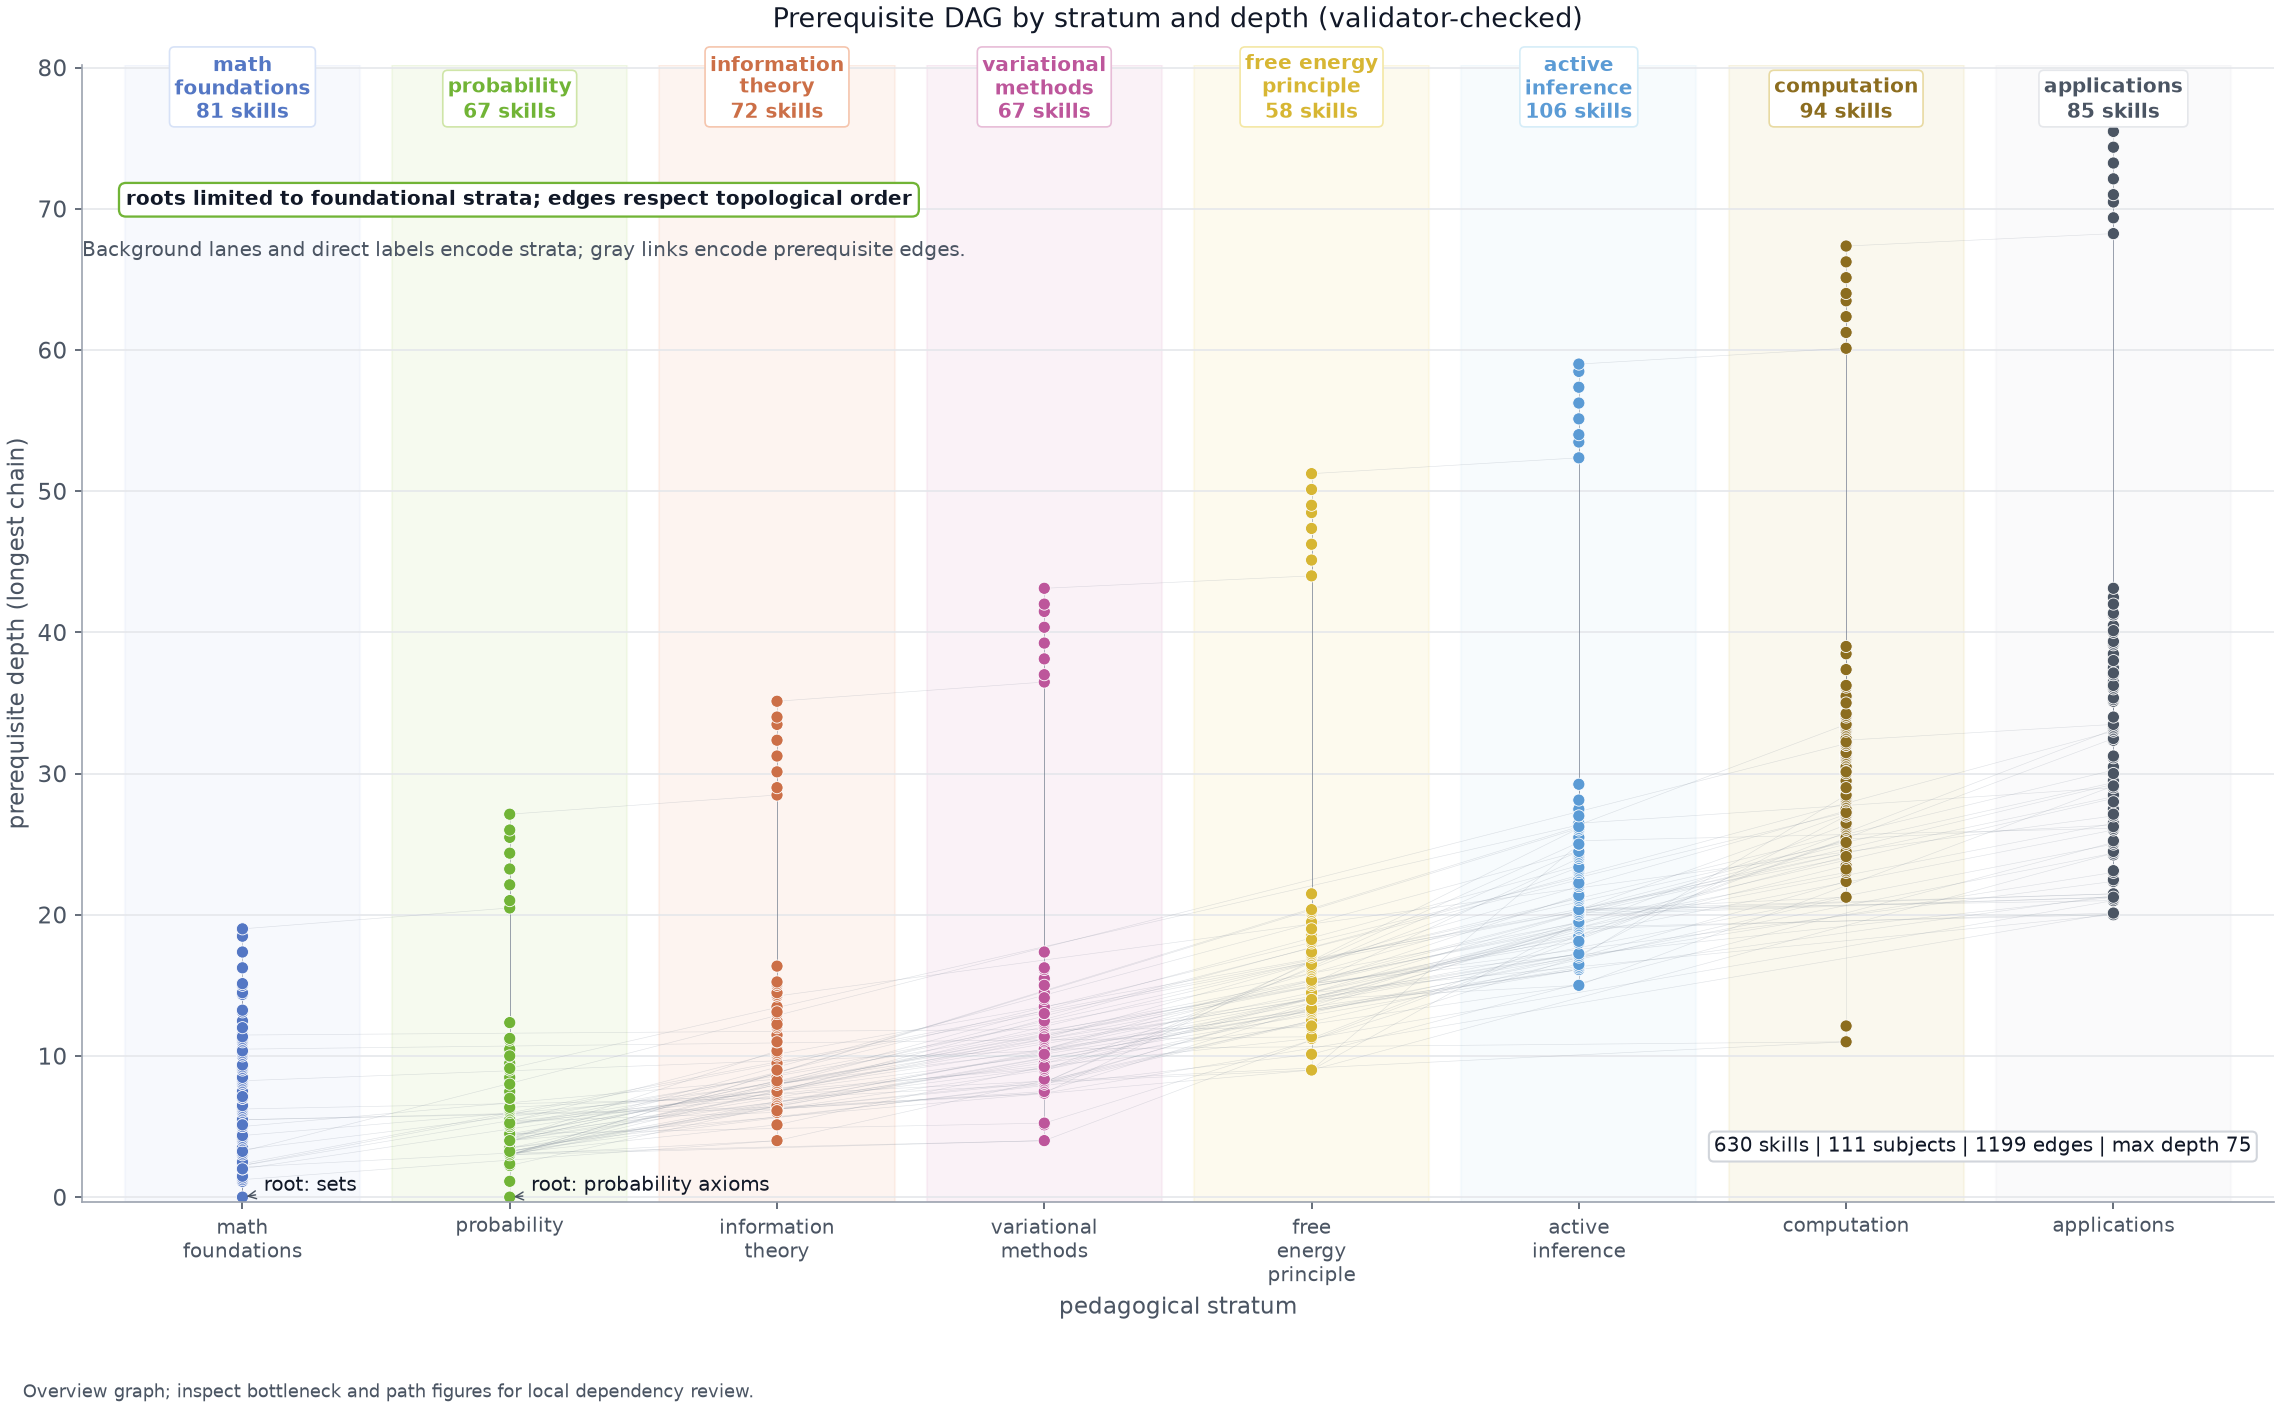
\includegraphics[width=1\linewidth,height=0.5\textheight,keepaspectratio,alt={The Active Inference curriculum as a prerequisite DAG generated from the current curriculum graph after structural checks. Each point is one skill, color encodes the pedagogical stratum, horizontal position follows the stratum order, vertical position follows longest prerequisite depth, and gray segments encode exported learning-path dependencies. Wrapped stratum chips report live skill totals, the two foundational roots are labeled, and the inset reports the live skill, subject, edge, and maximum-depth counts. This figure is an overview for structure and reachability; it does not by itself certify prose quality, assessment quality, or scholarship support.}]{../figures/curriculum_dag.png}
\caption{The Active Inference curriculum as a prerequisite DAG generated
from the current curriculum graph after structural checks. Each point is
one skill, color encodes the pedagogical stratum, horizontal position
follows the stratum order, vertical position follows longest
prerequisite depth, and gray segments encode exported learning-path
dependencies. Wrapped stratum chips report live skill totals, the two
foundational roots are labeled, and the inset reports the live skill,
subject, edge, and maximum-depth counts. This figure is an overview for
structure and reachability; it does not by itself certify prose quality,
assessment quality, or scholarship support.}\label{fig:curriculum_dag}
\end{figure}

The full DAG is the most faithful view, but it is intentionally dense:
learners need to see both the individual prerequisite chains and the
curriculum's aggregate traffic pattern.
fig.~\ref{fig:dependency_strata_flow} adds that second view. Rows are
prerequisite strata, columns are dependent strata, and the right-hand
bar gives the node count in each stratum. Diagonal cells show
within-stratum reinforcement; upper-triangular cells show forward
conceptual transitions. A populated lower-triangular cell would mean a
backward learning-path dependency, which the quality gate rejects before
export.

\begin{figure}
\centering
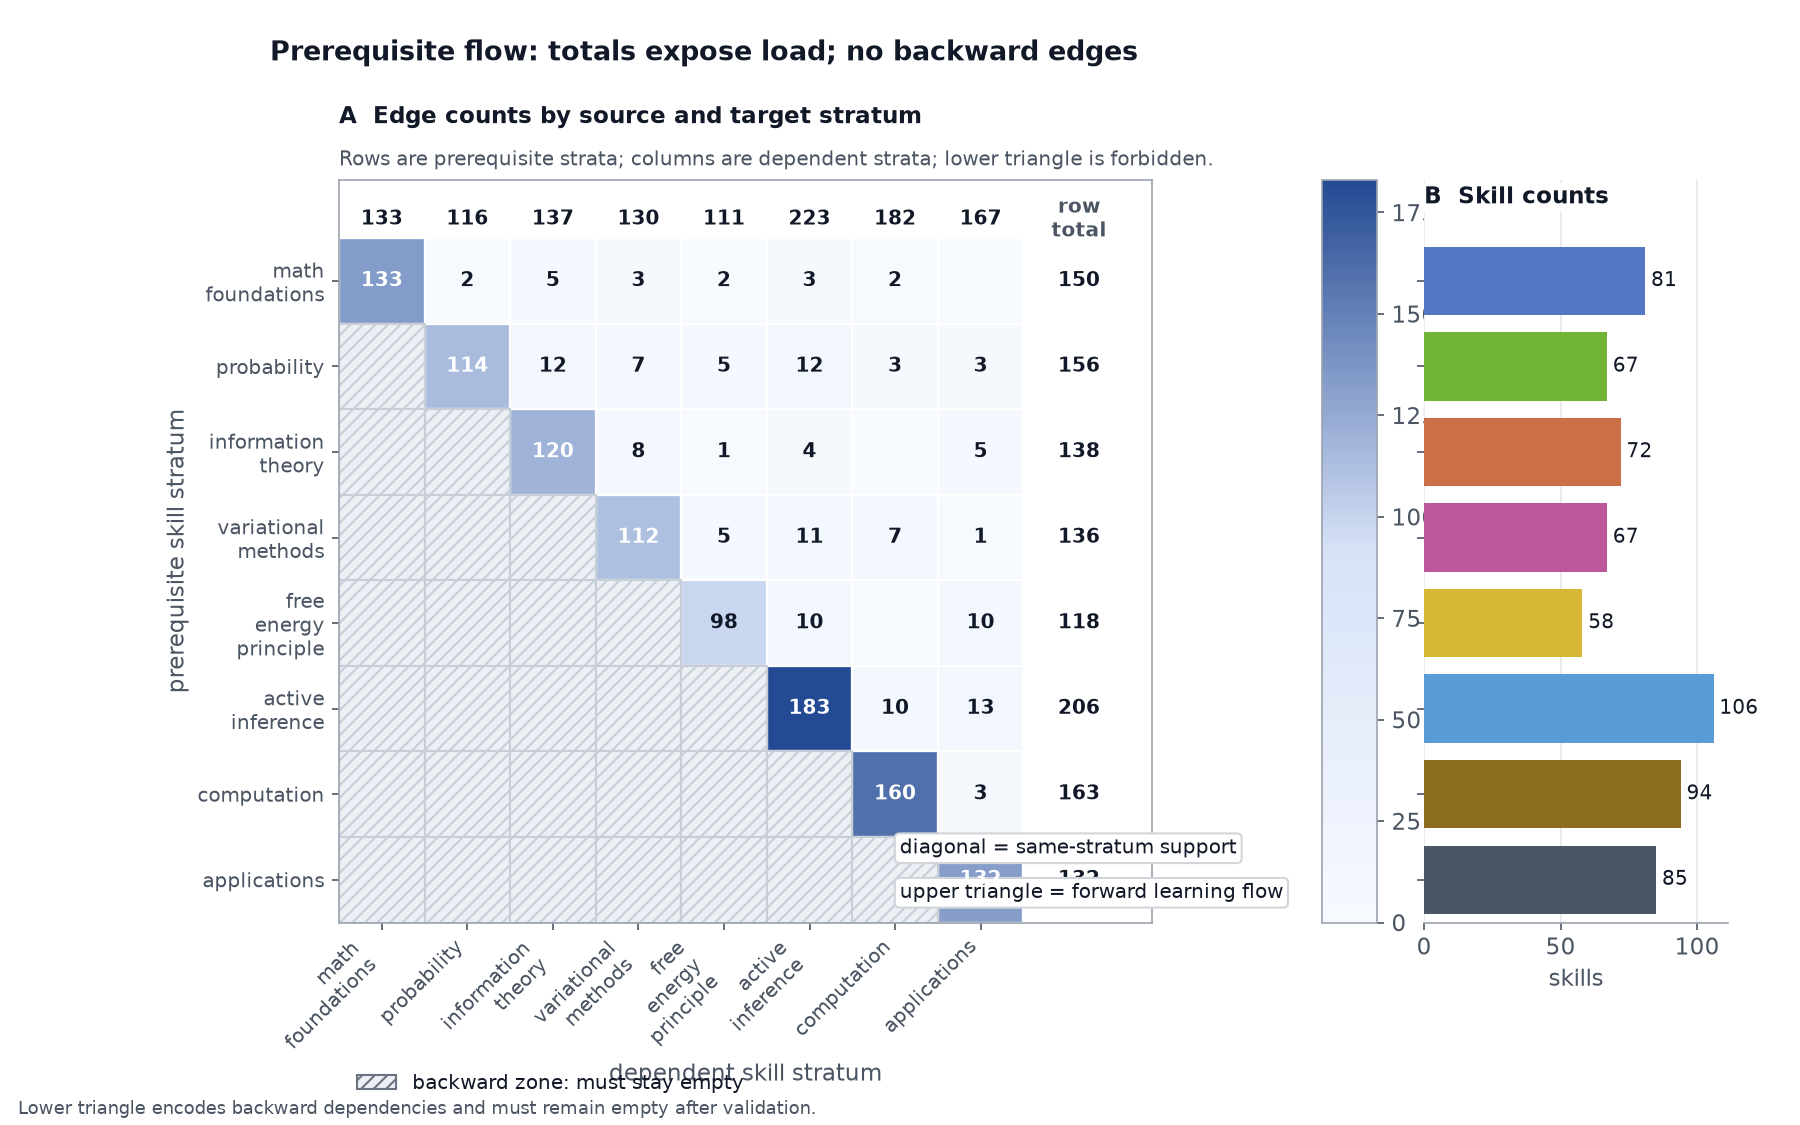
\includegraphics[width=0.95\linewidth,height=0.5\textheight,keepaspectratio,alt={Prerequisite-edge flow across strata generated from every exported learning-path edge. Rows are prerequisite strata, columns are dependent strata, cell labels count edges, and the side bar reports how many skills live in each stratum. Diagonal cells show within-stratum reinforcement, upper-triangular cells show forward conceptual transitions, and a populated lower-triangular cell would expose a backward prerequisite that should be rejected before export.}]{../figures/dependency_strata_flow.png}
\caption{Prerequisite-edge flow across strata generated from every
exported learning-path edge. Rows are prerequisite strata, columns are
dependent strata, cell labels count edges, and the side bar reports how
many skills live in each stratum. Diagonal cells show within-stratum
reinforcement, upper-triangular cells show forward conceptual
transitions, and a populated lower-triangular cell would expose a
backward prerequisite that should be rejected before
export.}\label{fig:dependency_strata_flow}
\end{figure}

The same graph also needs diagnostic views for authors.
fig.~\ref{fig:graph_bottlenecks} orders high-outdegree skills by how
much downstream curriculum they unlock, so review can focus on nodes
where a weak explanation would create wide learner risk.
fig.~\ref{fig:skill_neighborhood_paths} complements that global view
with a representative long dependency path. The figure keeps the route
line readable while a checkpoint ledger names the start, stratum
transitions, and endpoint, so a reader can inspect one concrete route
without zooming the full DAG or relying on angled micro-labels.

\begin{figure}
\centering
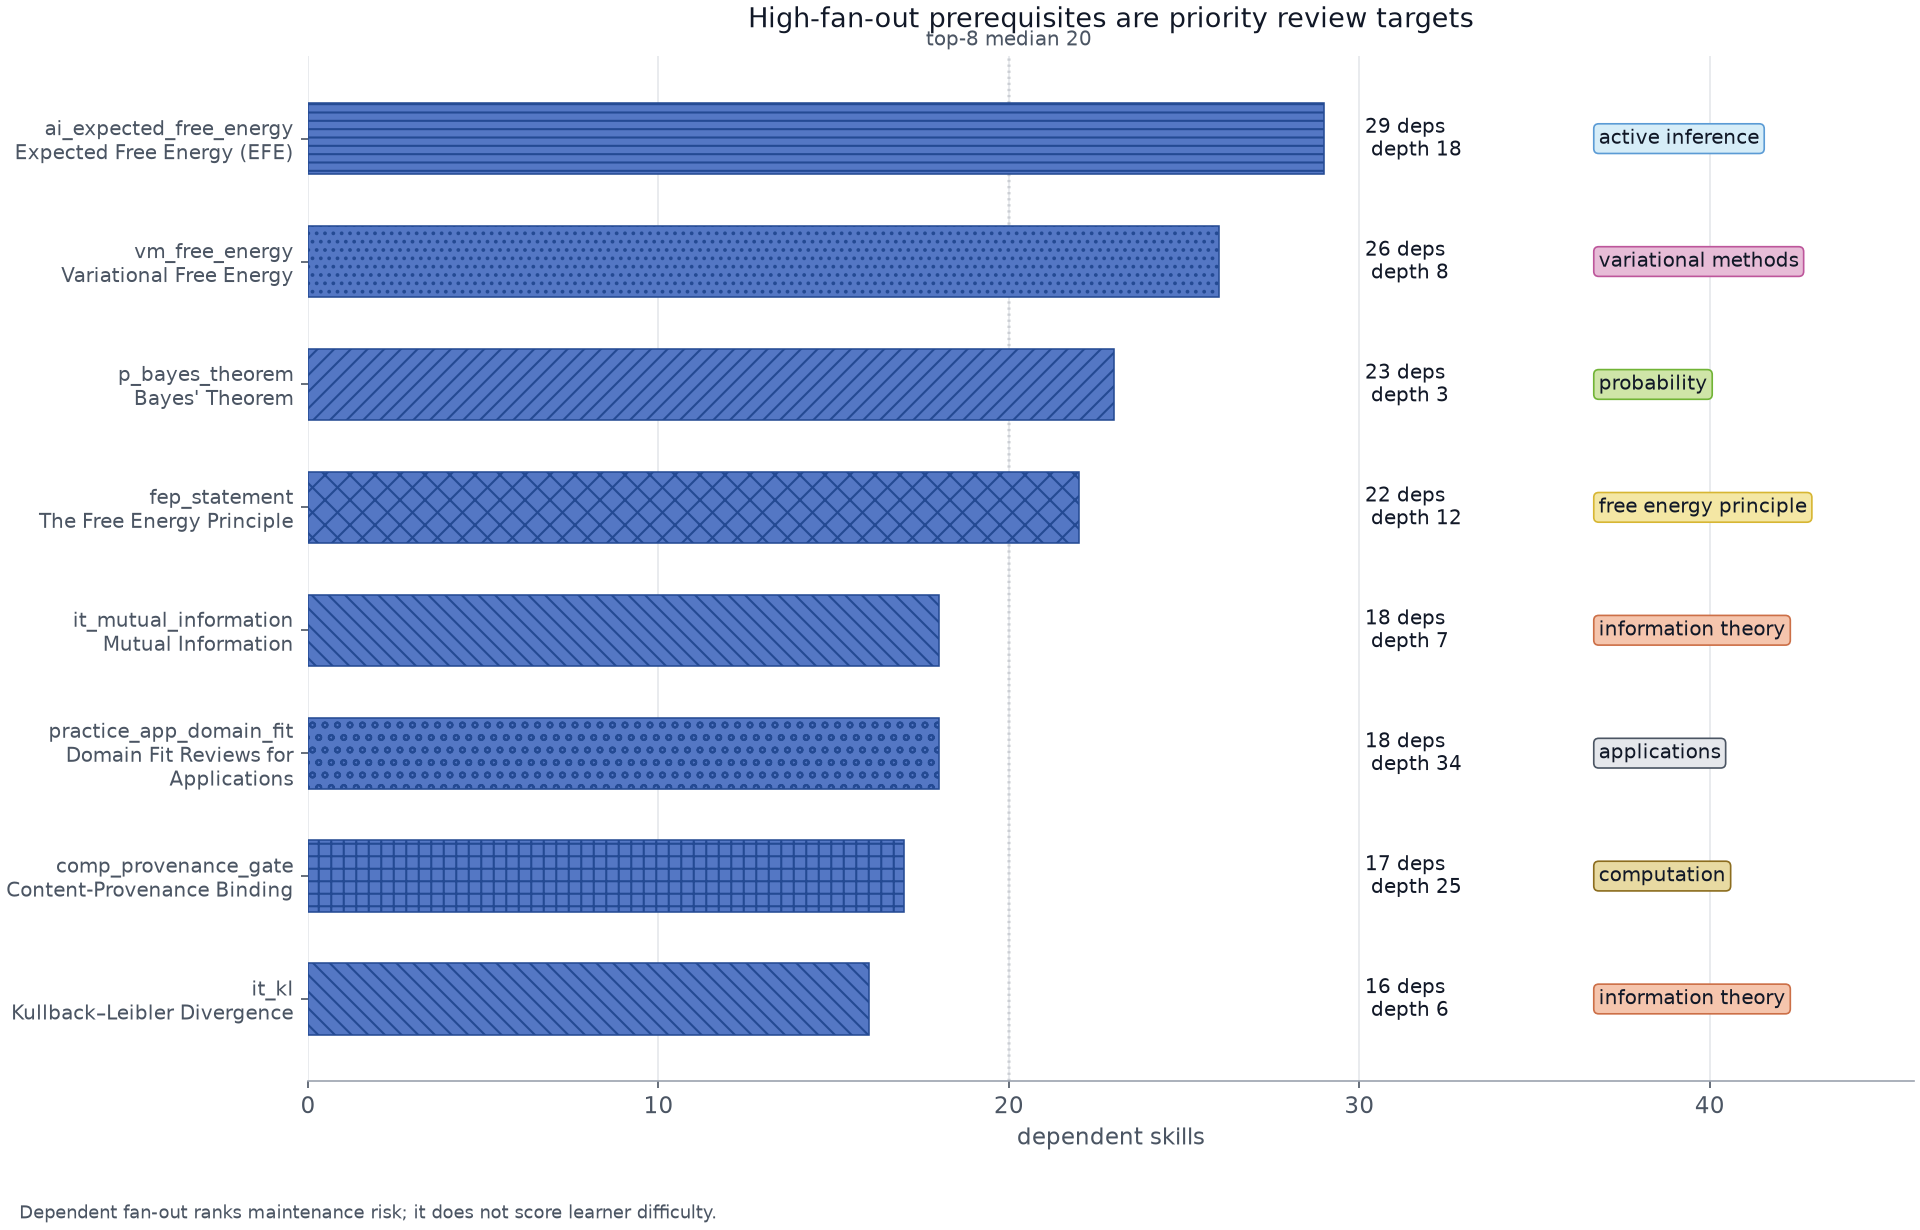
\includegraphics[width=0.92\linewidth,height=0.5\textheight,keepaspectratio,alt={Graph bottlenecks in the exported prerequisite network generated from downstream dependent counts. Bars rank the top fan-out skills, y-axis labels pair skill ids with readable names, hatching and stratum chips identify pedagogical layer, and annotations report dependent count and prerequisite depth for each high-impact node. The figure is a review-priority surface: it identifies where a weak explanation, stale citation, or thin quiz would propagate to many later skills even though the graph remains valid.}]{../figures/graph_bottlenecks.png}
\caption{Graph bottlenecks in the exported prerequisite network
generated from downstream dependent counts. Bars rank the top fan-out
skills, y-axis labels pair skill ids with readable names, hatching and
stratum chips identify pedagogical layer, and annotations report
dependent count and prerequisite depth for each high-impact node. The
figure is a review-priority surface: it identifies where a weak
explanation, stale citation, or thin quiz would propagate to many later
skills even though the graph remains
valid.}\label{fig:graph_bottlenecks}
\end{figure}

\begin{figure}
\centering
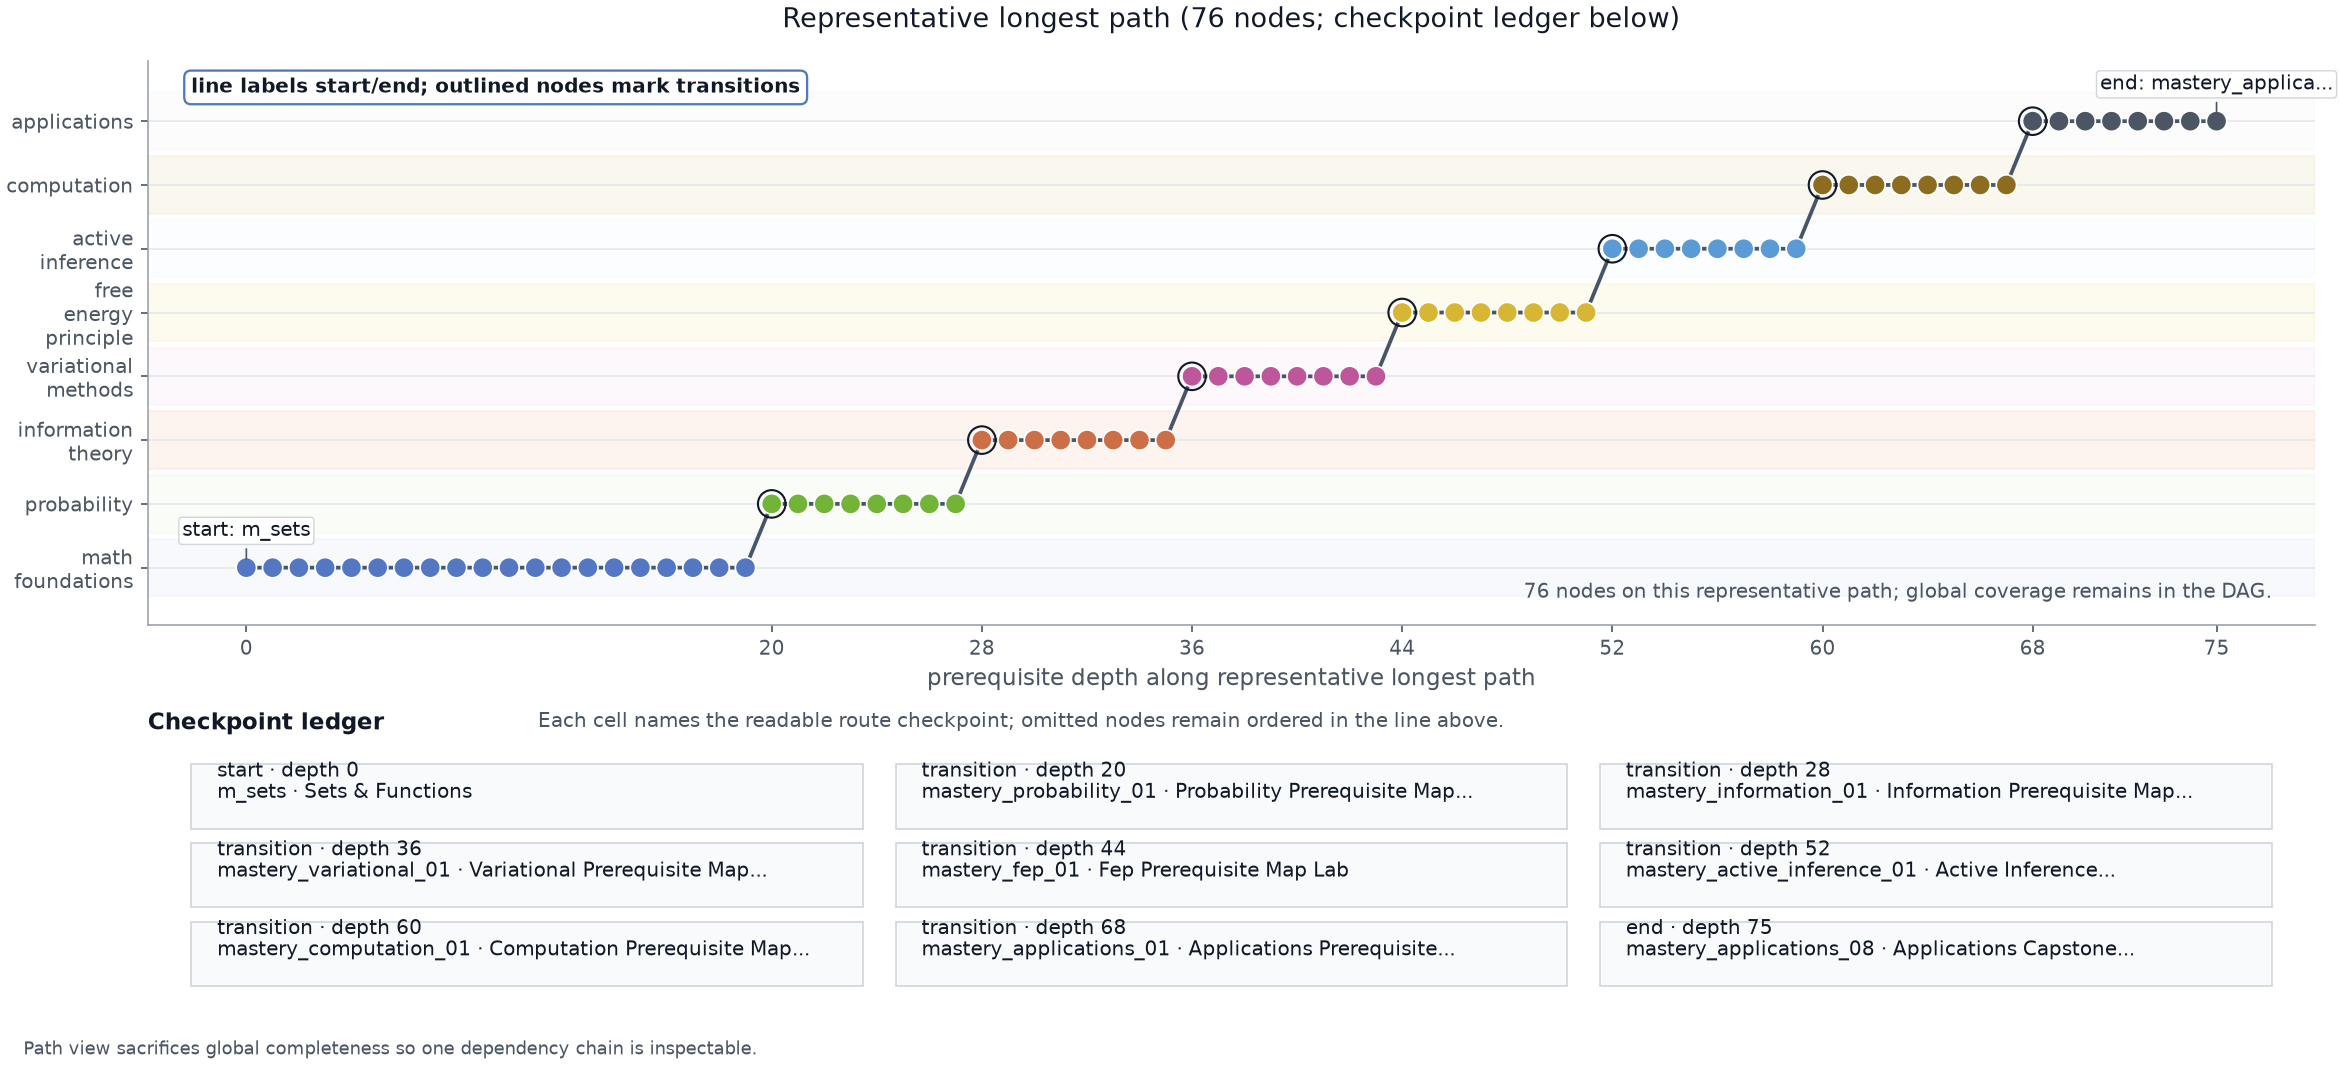
\includegraphics[width=1\linewidth,height=0.5\textheight,keepaspectratio,alt={Representative skill-neighborhood path generated from the longest-path diagnostic in the current graph. The line orders skills by prerequisite depth, stratum bands and vertical position encode pedagogical layer, and a checkpoint ledger names the start, every stratum transition, and the endpoint. This view deliberately trades global completeness for readability: it lets authors audit one concrete foundation-to-application pathway without relying on the dense full-DAG overview or tiny rotated labels.}]{../figures/skill_neighborhood_paths.png}
\caption{Representative skill-neighborhood path generated from the
longest-path diagnostic in the current graph. The line orders skills by
prerequisite depth, stratum bands and vertical position encode
pedagogical layer, and a checkpoint ledger names the start, every
stratum transition, and the endpoint. This view deliberately trades
global completeness for readability: it lets authors audit one concrete
foundation-to-application pathway without relying on the dense full-DAG
overview or tiny rotated labels.}\label{fig:skill_neighborhood_paths}
\end{figure}

fig.~\ref{fig:semantic_prerequisite_coverage} audits the
semantic-prerequisite gate, which checks that no skill is assessed on
one of the gate's tracked load-bearing concepts unless a skill defining
that concept sits in its transitive prerequisite closure. The gate reads
assessment text only, and it considers only definers at or before the
using skill's own stratum, so a forward reference to a later concept is
not counted as a missing prerequisite. For each concept the figure
reports how many skills reach the defining skill through their
prerequisite closure and how many are assessed on the concept, so an
inversion in which a learner met a concept before they could have
learned it would be visible rather than buried in the dense graph.

\begin{figure}
\centering
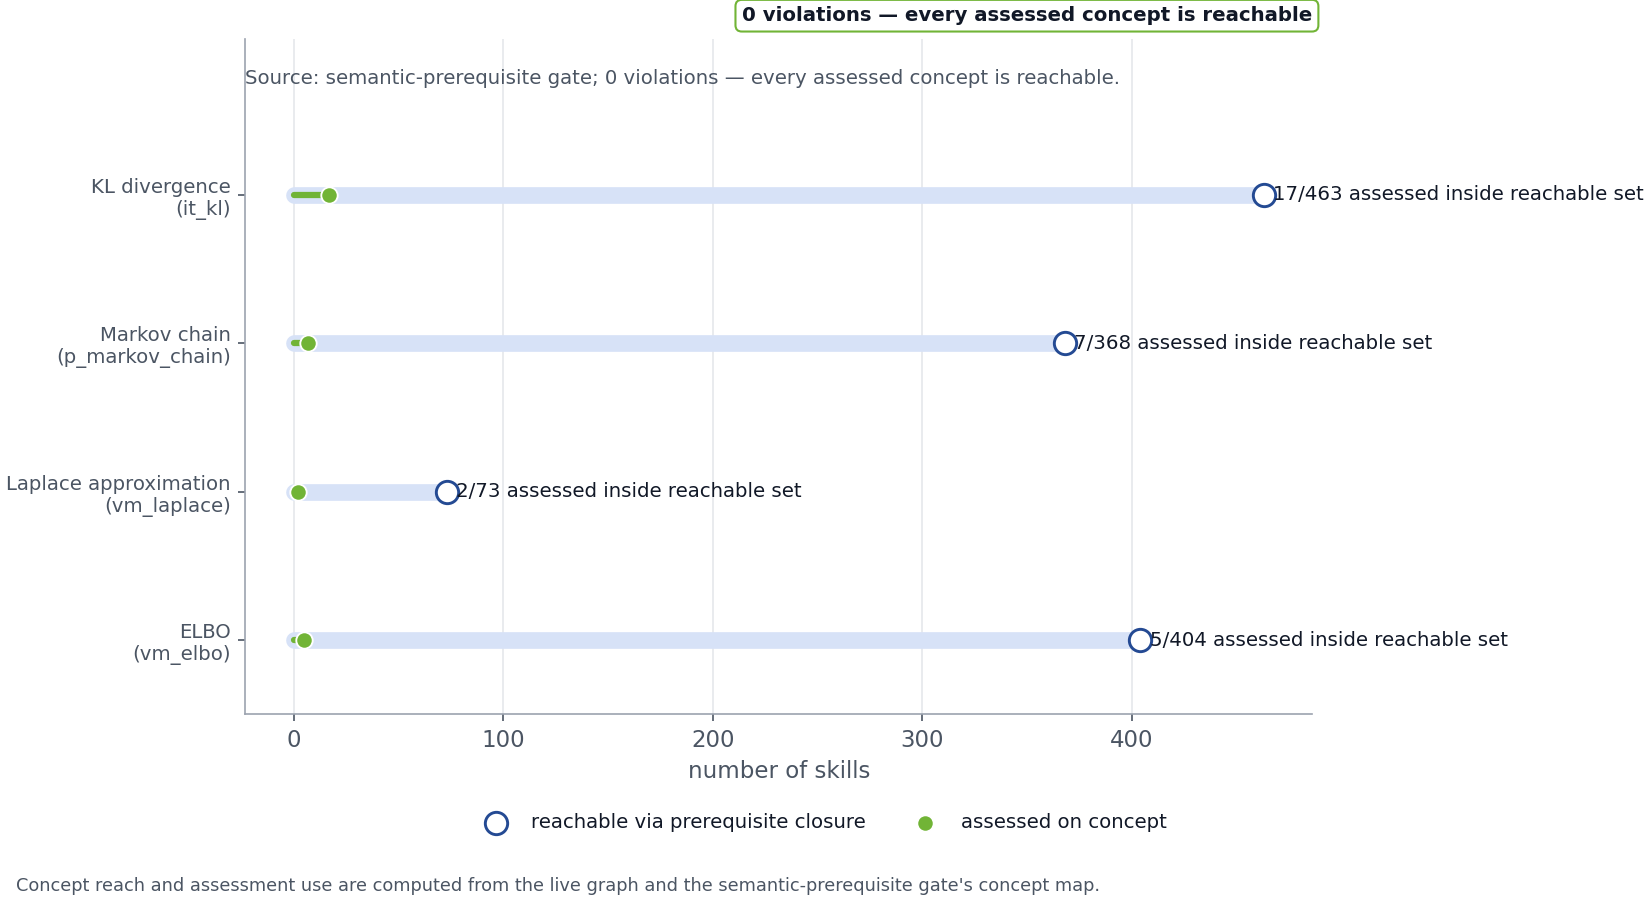
\includegraphics[width=0.92\linewidth,height=0.5\textheight,keepaspectratio,alt={Semantic-prerequisite coverage generated from the live graph and the quality gate's concept map. For each load-bearing concept the open marker and stem report skills whose prerequisite closure reaches the concept's defining skill, while the filled marker and direct label report the assessed subset inside that reachable set. The subtitle and badge report the gate verdict so a passing curriculum shows zero skills tested on a concept they could not yet have learned.}]{../figures/semantic_prerequisite_coverage.png}
\caption{Semantic-prerequisite coverage generated from the live graph
and the quality gate's concept map. For each load-bearing concept the
open marker and stem report skills whose prerequisite closure reaches
the concept's defining skill, while the filled marker and direct label
report the assessed subset inside that reachable set. The subtitle and
badge report the gate verdict so a passing curriculum shows zero skills
tested on a concept they could not yet have
learned.}\label{fig:semantic_prerequisite_coverage}
\end{figure}

The quiz surface is itself part of the curriculum result rather than a
decorative add-on. fig.~\ref{fig:assessment_depth} summarizes the
assessment-depth invariant by stratum. Every skill now carries the same
4-question floor, so completion is not certified by a single recognition
item or by a thin two-question check.

\begin{figure}
\centering
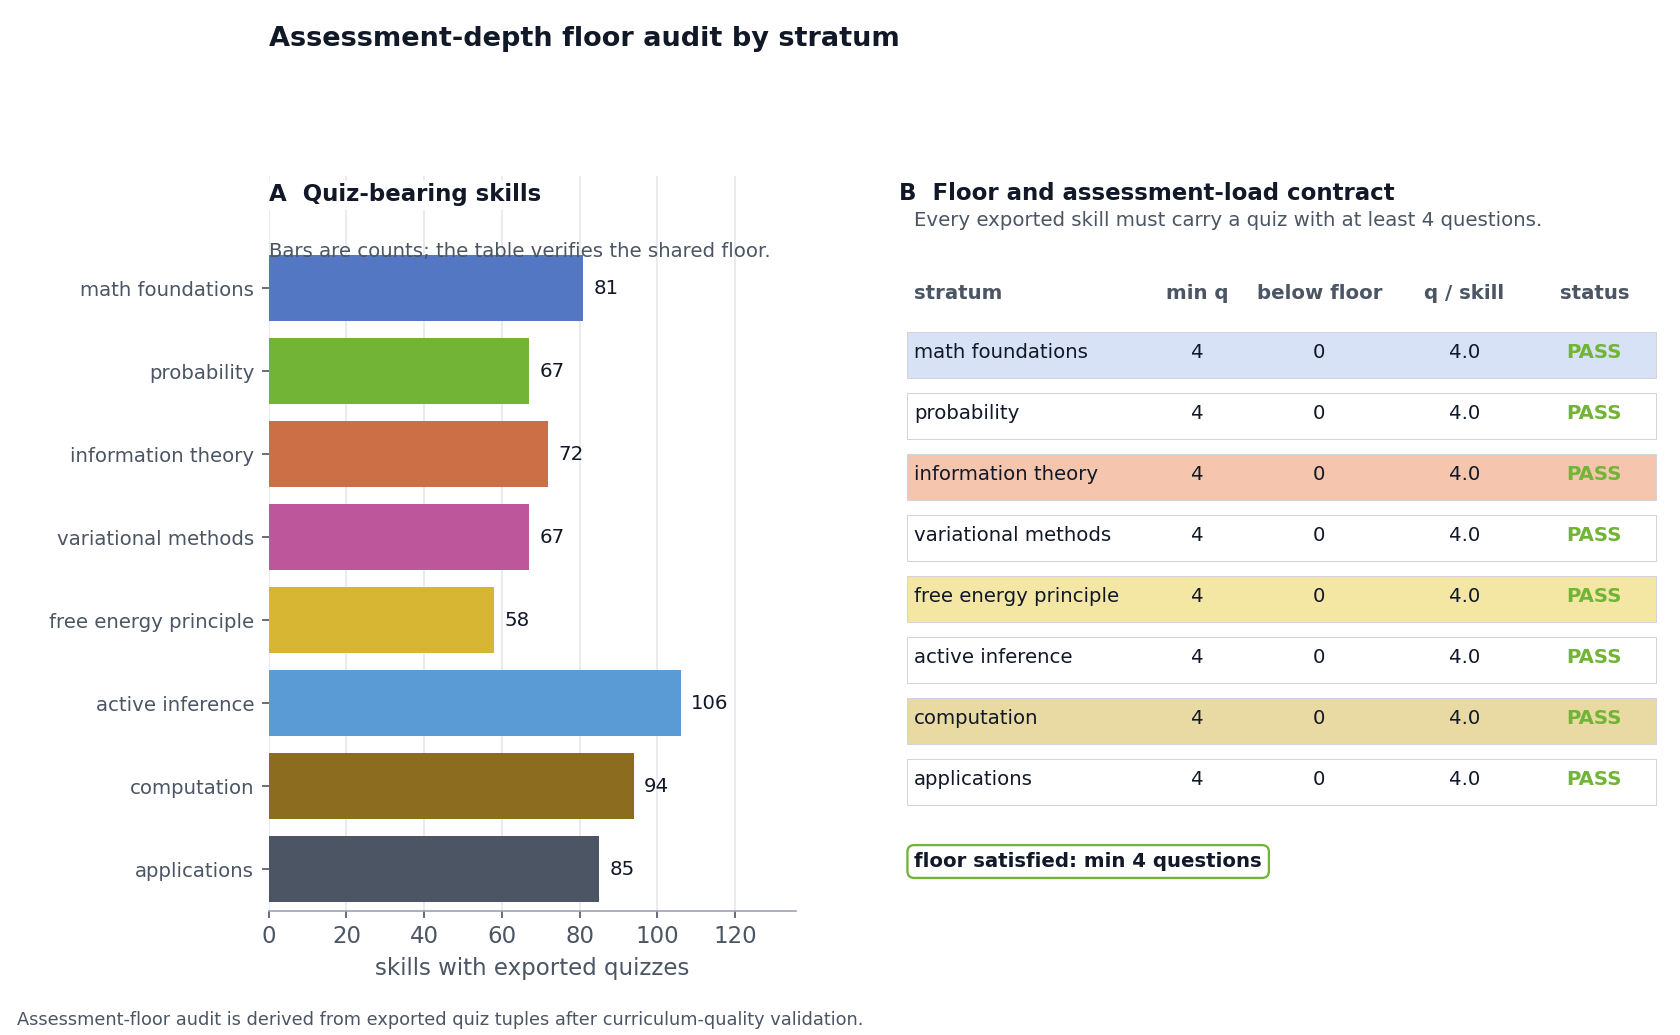
\includegraphics[width=0.9\linewidth,height=0.5\textheight,keepaspectratio,alt={Quiz assessment depth by stratum generated from the skill assessment tuples. The bar panel counts quiz-bearing skills per pedagogical stratum, and the accompanying audit table reports, per stratum, the minimum questions per skill, below-floor counts, questions per skill, and a PASS/REVIEW verdict against the configured 4-question failable floor. The intended check is not average quiz length but minimum learner friction: any below-floor mass would show that a skill can be completed without the configured 4-question floor.}]{../figures/assessment_depth_matrix.png}
\caption{Quiz assessment depth by stratum generated from the skill
assessment tuples. The bar panel counts quiz-bearing skills per
pedagogical stratum, and the accompanying audit table reports, per
stratum, the minimum questions per skill, below-floor counts, questions
per skill, and a PASS/REVIEW verdict against the configured 4-question
failable floor. The intended check is not average quiz length but
minimum learner friction: any below-floor mass would show that a skill
can be completed without the configured 4-question
floor.}\label{fig:assessment_depth}
\end{figure}

The latest expansion also needs a balance check.
fig.~\ref{fig:stratum_balance} summarizes skills, subjects, assessment
questions and incoming prerequisite edges by stratum. This makes a
different false-certification path visible: the graph can be larger
while still overloading one pedagogical layer or leaving another
underdeveloped.

\begin{figure}
\centering
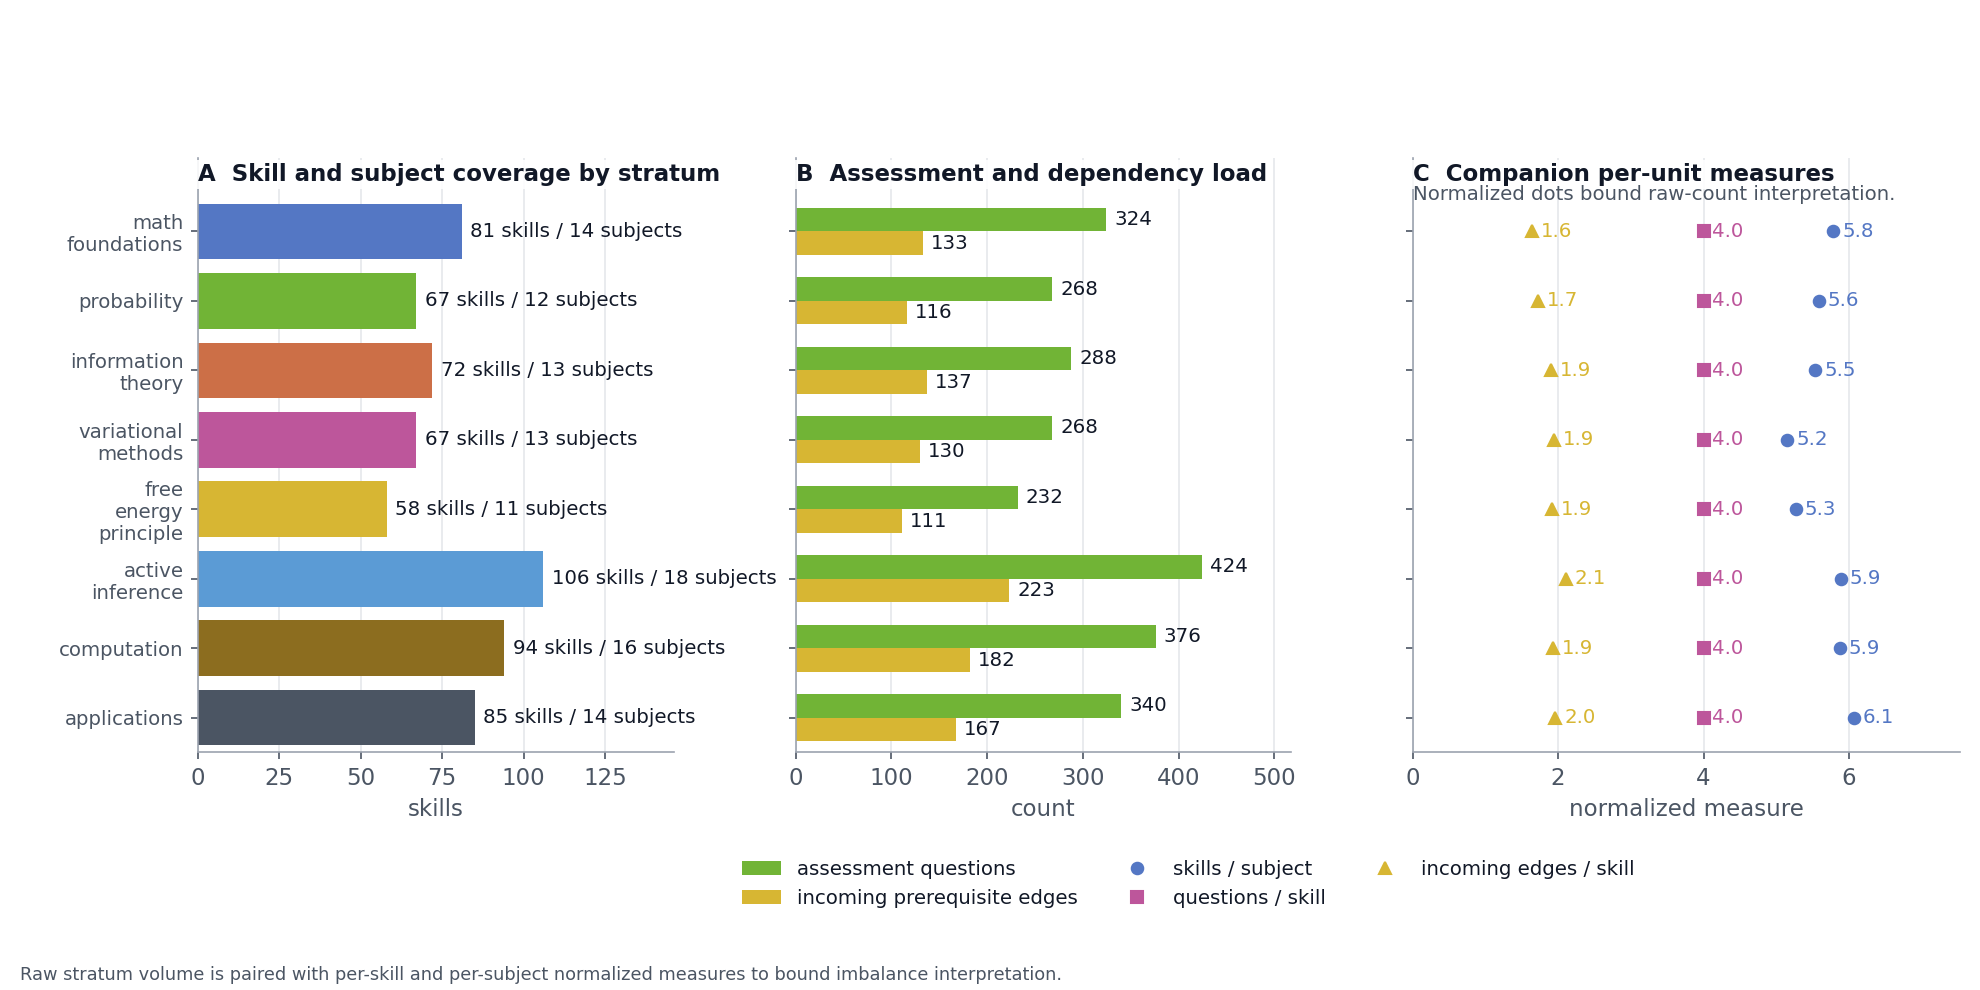
\includegraphics[width=1\linewidth,height=0.5\textheight,keepaspectratio,alt={Curriculum stratum-balance audit generated from current graph statistics after structural checks. Three panels report the same underlying build: the left panel shows skills and subjects per pedagogical stratum, the middle panel shows assessment-question volume and incoming prerequisite edges, and the right panel shows companion per-unit (per-skill and per-subject) normalized measures. Reading the panels together shows whether expansion is distributed across the learning path or whether one layer is absorbing disproportionate topic, quiz, or dependency load. The figure bounds the claim to catalog structure; it does not measure learner outcomes.}]{../figures/curriculum_stratum_balance.png}
\caption{Curriculum stratum-balance audit generated from current graph
statistics after structural checks. Three panels report the same
underlying build: the left panel shows skills and subjects per
pedagogical stratum, the middle panel shows assessment-question volume
and incoming prerequisite edges, and the right panel shows companion
per-unit (per-skill and per-subject) normalized measures. Reading the
panels together shows whether expansion is distributed across the
learning path or whether one layer is absorbing disproportionate topic,
quiz, or dependency load. The figure bounds the claim to catalog
structure; it does not measure learner
outcomes.}\label{fig:stratum_balance}
\end{figure}

Having established the graph surface, the next result is source support.
These audits ask whether the manuscript's scholarly claims are connected
to the roles its citations are supposed to play.

\newpage

\section{Results: Scholarship Coverage and Evidence-Status
Audits}\label{sec:results-scholarship-source-health-evidence}

\subsection{Citation coverage, locator health, and evidence-class
auditing}\label{citation-coverage-locator-health-and-evidence-class-auditing}

The manuscript's source coverage is also treated as a generated result.
Every authored citation is parsed from the section files, matched
against \texttt{references.bib}, and mapped through
\breaktt{data/scholarship\_sources.yaml} into a source lane and support
role before the build writes figures. The current audit covers 188 cited
sources; that number is generated from the manuscript and source matrix,
not maintained as a prose claim. fig.~\ref{fig:scholarship_coverage}
shows both sides of the contract: the left panel compares cited sources
with the matrixed source pool for each lane, while the right panel shows
which manuscript sections carry each lane. The audit is deliberately
orthogonal to the numeric claim registry: one gate protects computed
quantities; the other protects the scholarly support surface.

\begin{figure}
\centering
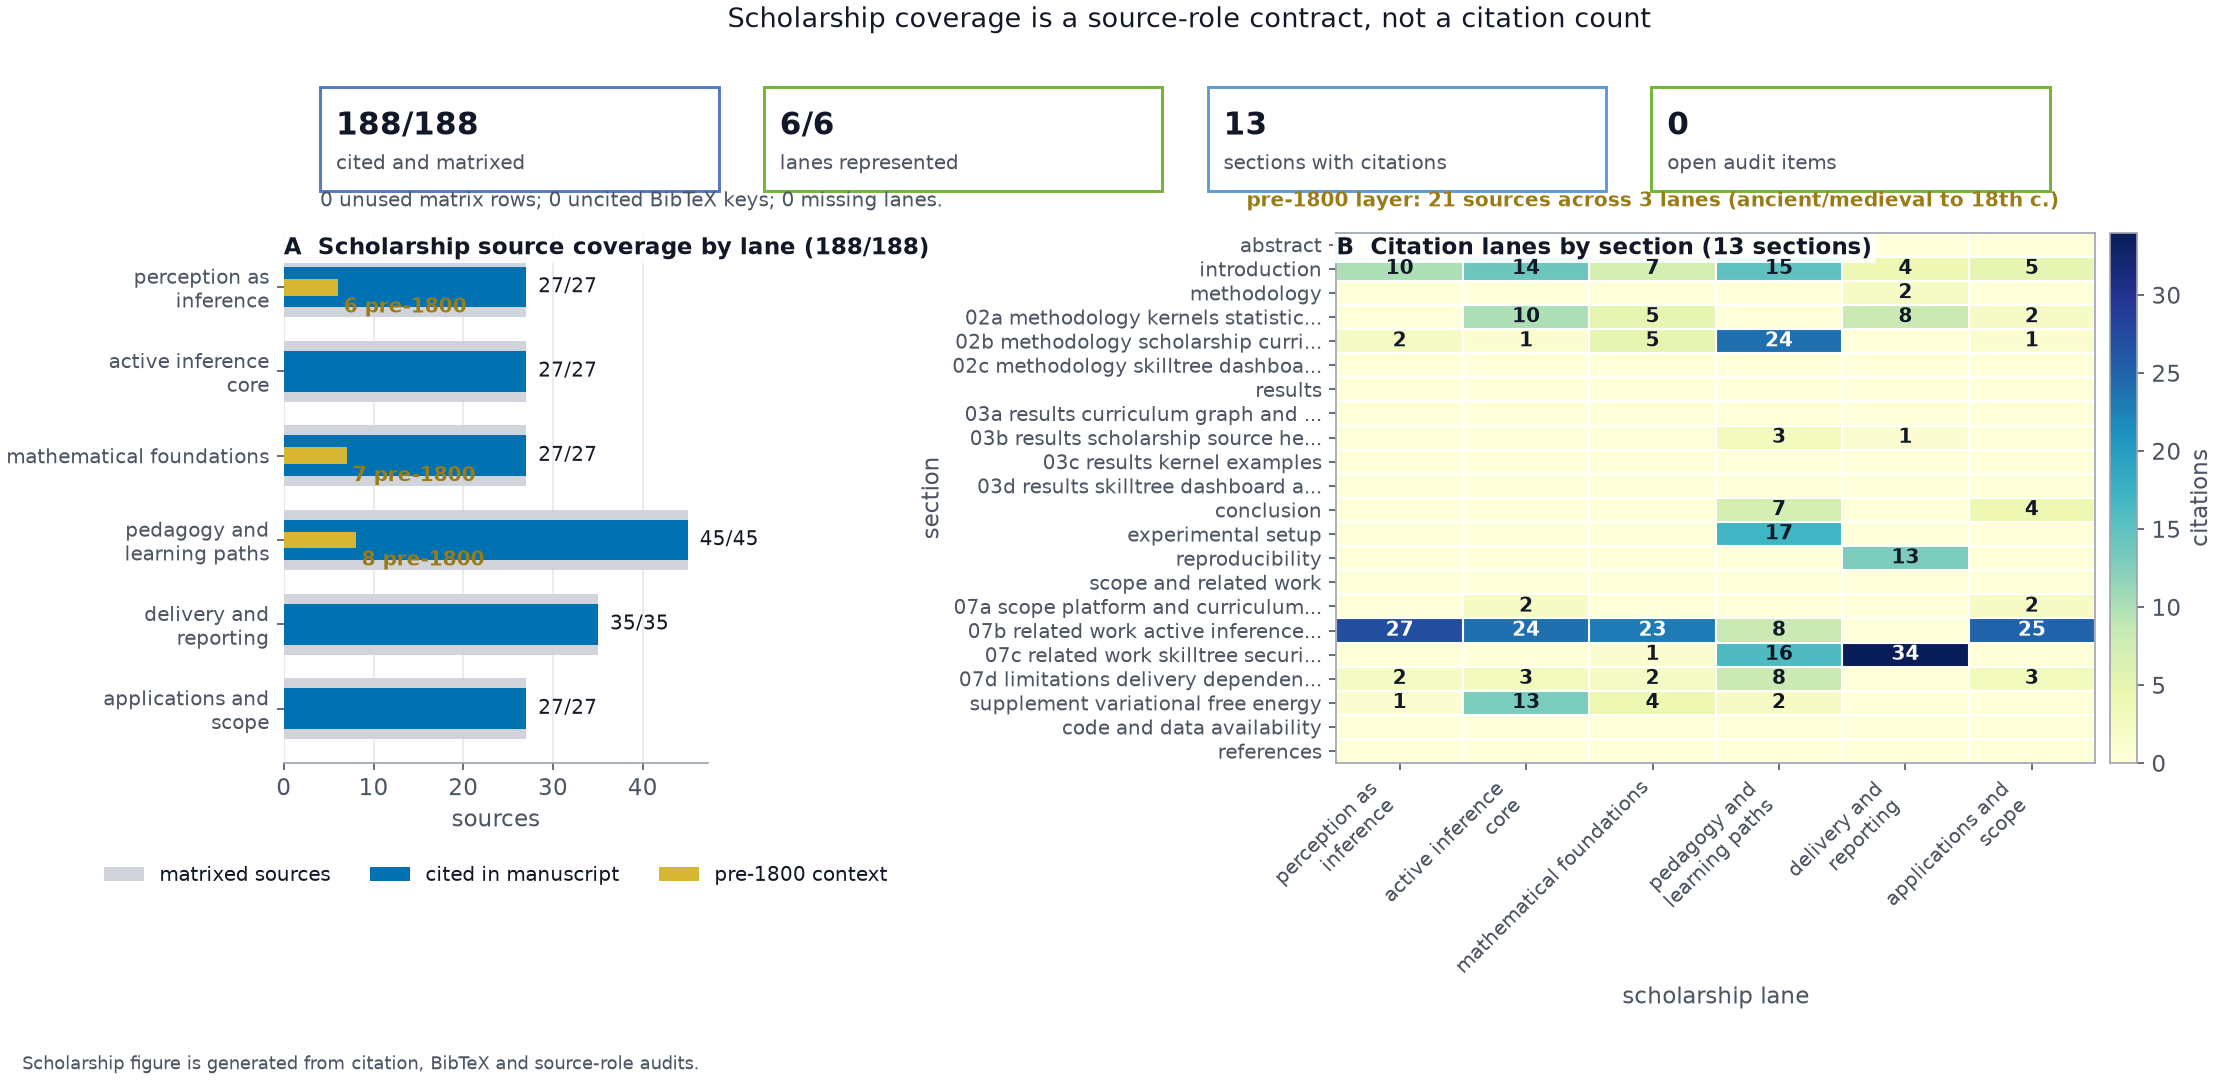
\includegraphics[width=1\linewidth,height=0.5\textheight,keepaspectratio,alt={Scholarship coverage audit generated from manuscript citations, BibTeX keys, and the source-role matrix. The left panel compares cited versus matrixed sources by scholarship lane; the right panel maps manuscript sections to citation lanes. This figure makes support distribution inspectable: a large bibliography is not treated as sufficient unless sources are cited in the sections and roles where they support specific claims.}]{../figures/scholarship_coverage.png}
\caption{Scholarship coverage audit generated from manuscript citations,
BibTeX keys, and the source-role matrix. The left panel compares cited
versus matrixed sources by scholarship lane; the right panel maps
manuscript sections to citation lanes. This figure makes support
distribution inspectable: a large bibliography is not treated as
sufficient unless sources are cited in the sections and roles where they
support specific claims.}\label{fig:scholarship_coverage}
\end{figure}

The open-science education layer is also explicit. Active Skillference
cites the Active Inference Institute's public education ecosystem,
including the open-source course infrastructure, the START
curriculum-generation project, and the Institute website's open-science
educational mission
\citep{activeinferenceinstitute2026courses, activeinferenceinstitute2026start, activeinferenceinstitute2026home}.
The generated local Learn material also links every exported skill to
commit-pinned external material pointers, including the Active Inference
Institute cognitive knowledge base
\citep{activeinferenceinstitute2026cognitive}.
fig.~\ref{fig:open_science_sources} shows both surfaces together: cited
public sources remain visible, and the course-material source rows
expose how the cognitive knowledge base enters the generated skill
records.

\begin{figure}
\centering
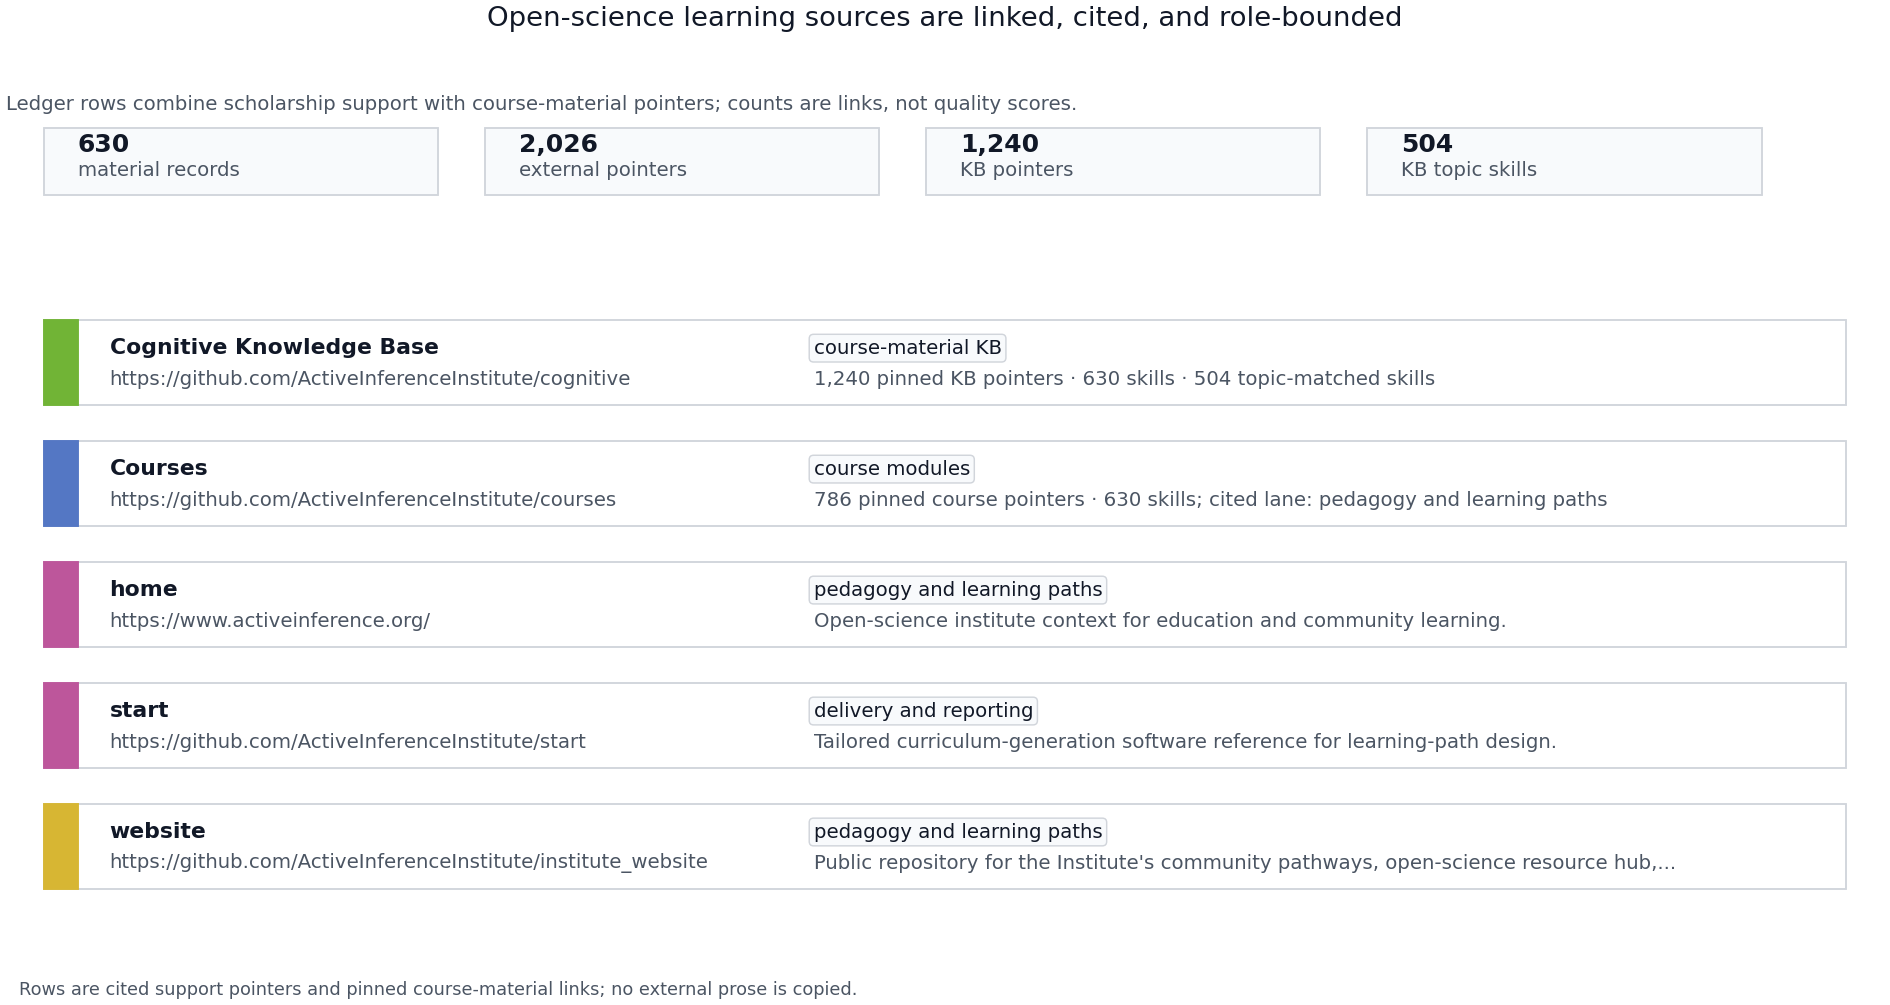
\includegraphics[width=0.88\linewidth,height=0.5\textheight,keepaspectratio,alt={Active Inference Institute open-science learning sources across scholarship support and generated course-material pointers. Summary cards report local material records, external pointers, cognitive knowledge-base pointers, and topic-matched KB skills; ledger rows distinguish the course repository, cognitive knowledge-base source, Institute homepage, website repository, and START source with locator and role text. The website repository is a community/resource-hub pointer rather than a course or knowledge-base record. The figure records pinned links and cited support surfaces; it does not claim endorsement, completeness, or copied ownership of the public education ecosystem.}]{../figures/open_science_source_map.png}
\caption{Active Inference Institute open-science learning sources across
scholarship support and generated course-material pointers. Summary
cards report local material records, external pointers, cognitive
knowledge-base pointers, and topic-matched KB skills; ledger rows
distinguish the course repository, cognitive knowledge-base source,
Institute homepage, website repository, and START source with locator
and role text. The website repository is a community/resource-hub
pointer rather than a course or knowledge-base record. The figure
records pinned links and cited support surfaces; it does not claim
endorsement, completeness, or copied ownership of the public education
ecosystem.}\label{fig:open_science_sources}
\end{figure}

The source matrix is then checked a second way: source locators must be
syntactically specific, documentation entries must use URL locators, and
each support role must be substantive enough to explain why the source
is present. fig.~\ref{fig:scholarship_source_health} reports the
resulting offline source-health audit and provides a place for optional
online DOI/URL reachability checks to surface when release review
requires currentness evidence.

\begin{figure}
\centering
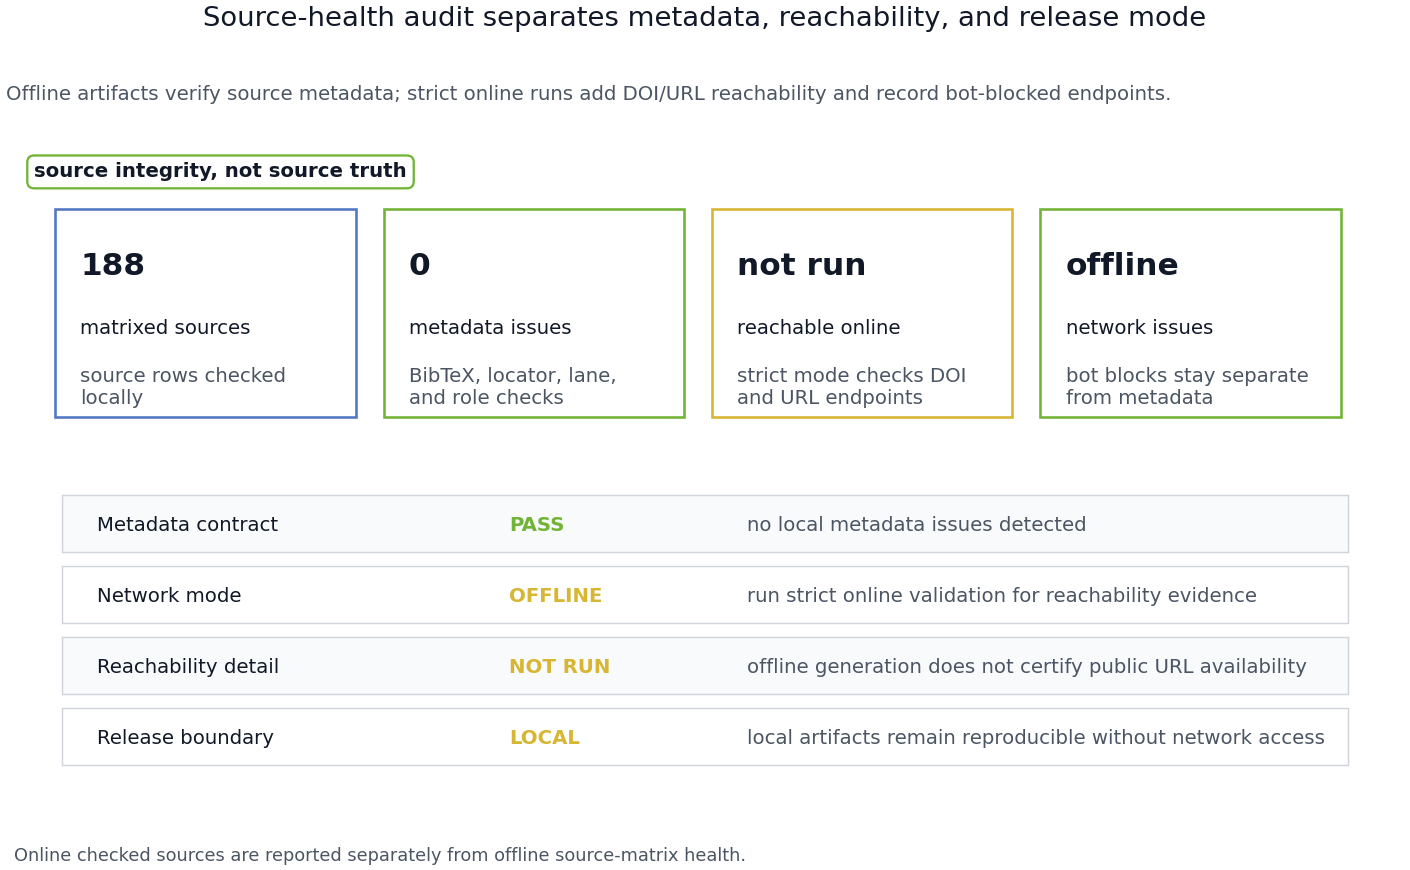
\includegraphics[width=0.88\linewidth,height=0.5\textheight,keepaspectratio,alt={Scholarship source-health audit generated from locator syntax, lane assignment, and support-role checks. Status cards separate matrixed source count, offline validation issues, and online-check mode, while the ledger rows distinguish local metadata health from optional network reachability. The figure separates two different claims: a source can be present in the matrix and still require locator, role, or currentness repair before release.}]{../figures/scholarship_source_health.png}
\caption{Scholarship source-health audit generated from locator syntax,
lane assignment, and support-role checks. Status cards separate matrixed
source count, offline validation issues, and online-check mode, while
the ledger rows distinguish local metadata health from optional network
reachability. The figure separates two different claims: a source can be
present in the matrix and still require locator, role, or currentness
repair before release.}\label{fig:scholarship_source_health}
\end{figure}

The validation surface is intentionally visible rather than left as a
hidden CI detail. fig.~\ref{fig:validation_surface_matrix} summarizes
which gates bind generated JSON, negative controls, manuscript text,
dashboard artifacts, release documentation, and SkillTree handoffs. Its
count panel is rebuilt from the same graph, claim registry, scholarship
audit and roadmap state that produce the curriculum and manuscript
variables. The result is a falsifiable release claim: if a count,
citation, figure, dashboard artifact, release inventory row, or roadmap
item drifts away from its generator, the validator fails before the
manuscript or SkillTree export can be presented as current.

\begin{figure}
\centering
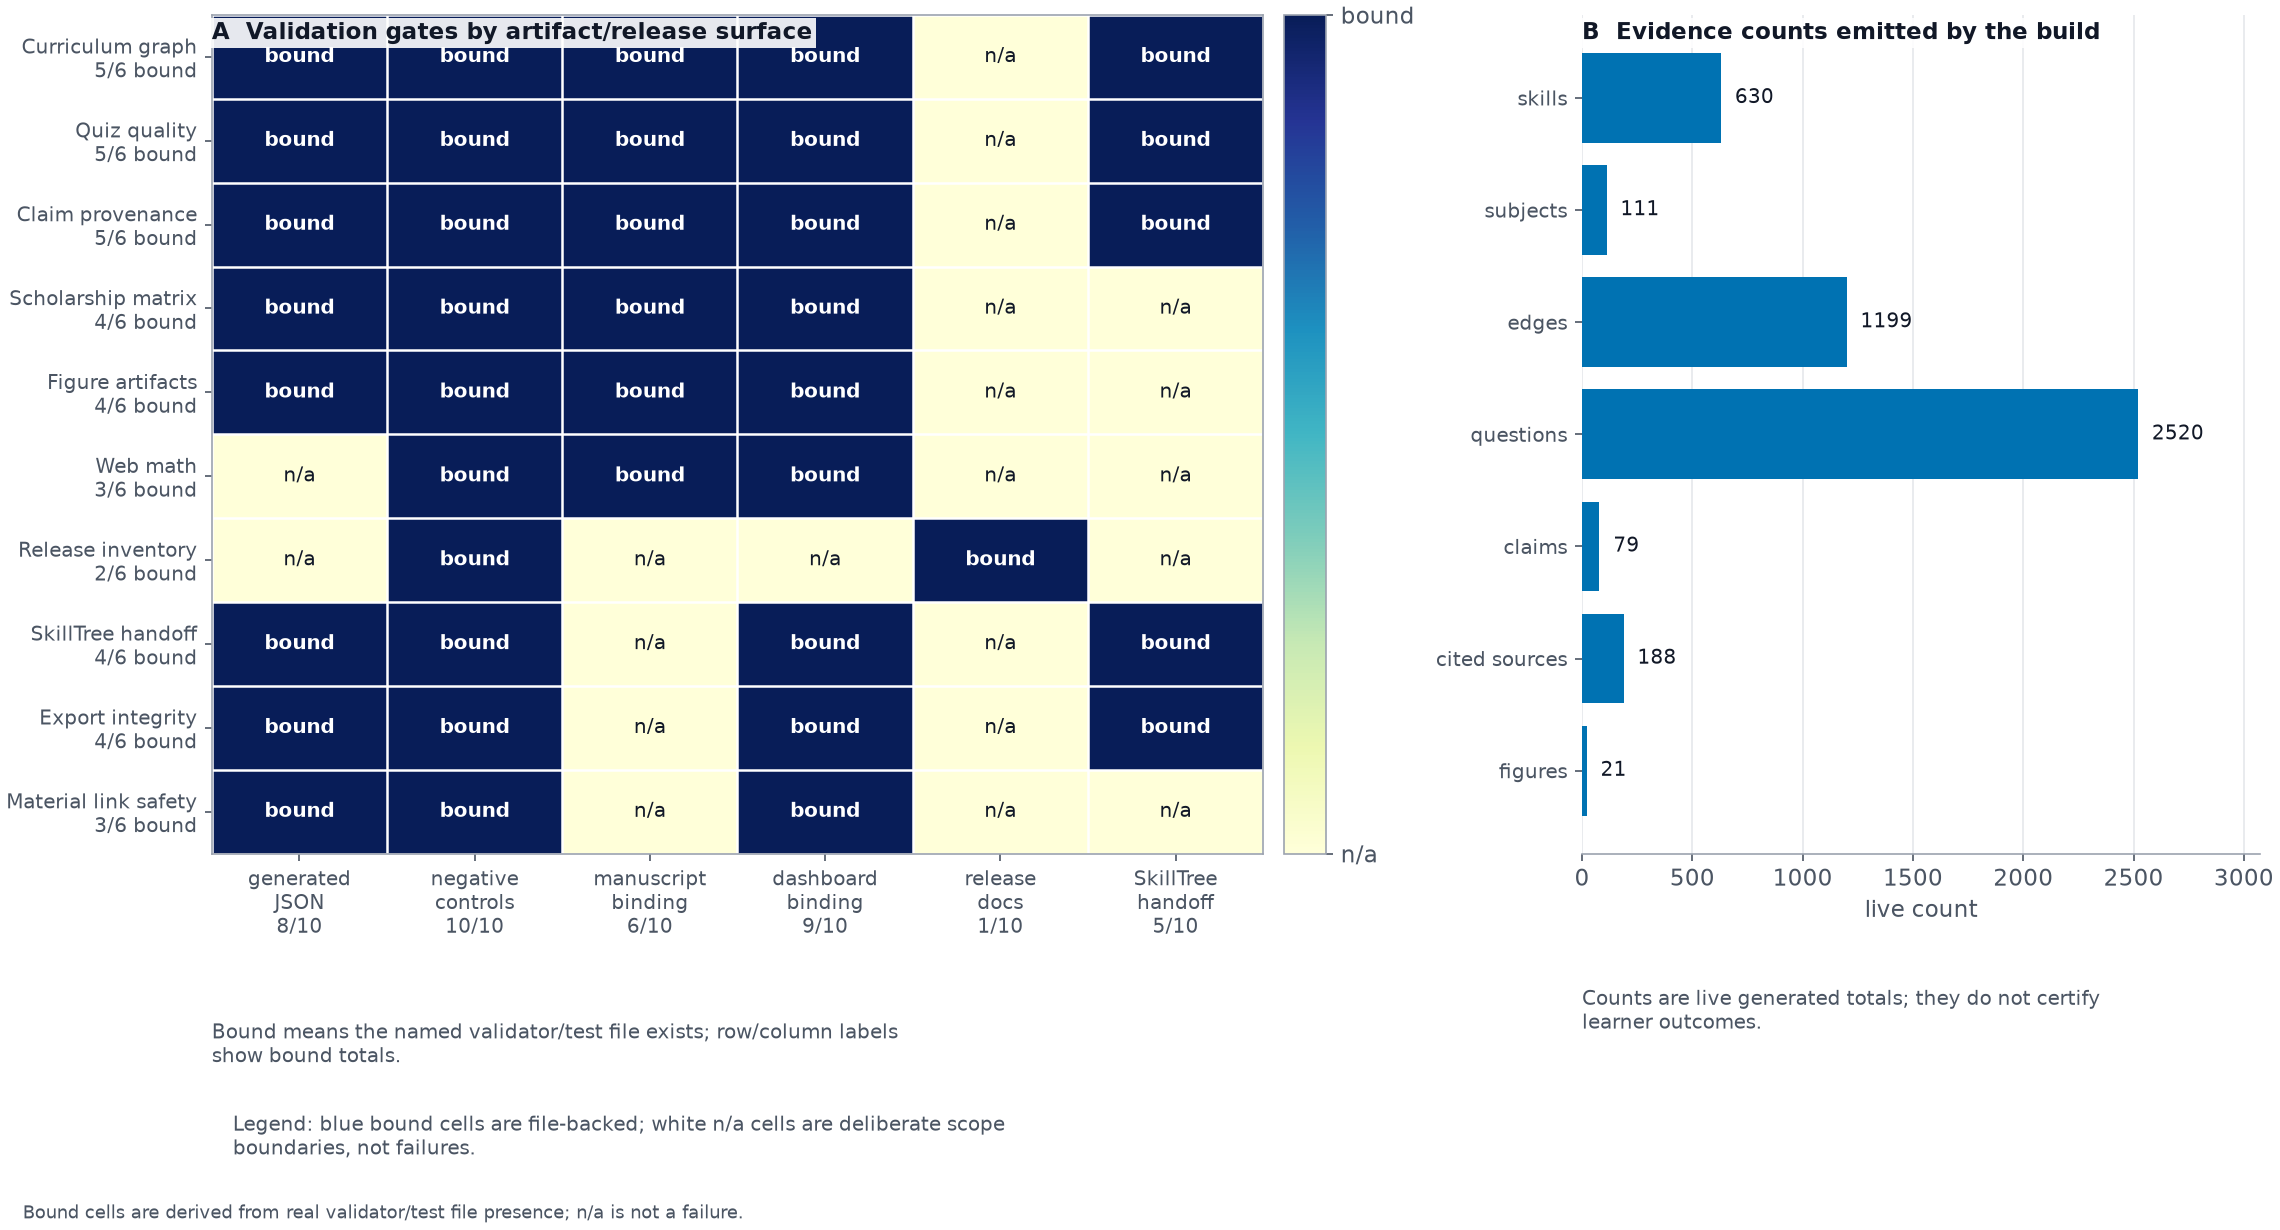
\includegraphics[width=1\linewidth,height=0.5\textheight,keepaspectratio,alt={Validation-surface matrix for Active Skillference. Each cell is derived from the on-disk presence of the validator or test file that binds that artifact surface: a cell reads ``bound'' only when every file named in its binding exists, so deleting a gate flips its cell to ``n/a'' rather than leaving a stale ``bound'' claim. Row and column labels state bound-cell totals, and each cell carries text, so the figure remains readable without heatmap color. The side panel reports live evidence counts for skills, subjects, dependencies, assessment questions, claims, cited sources, and registered figures, read directly from the graph, claim registry, scholarship audit, and figure inventory. The interpretation boundary is important: a bound cell means a named validator file exists for that artifact surface (not that the gate is guaranteed sound), while an unbound cell marks a surface that is out of scope for that gate.}]{../figures/validation_surface_matrix.png}
\caption{Validation-surface matrix for Active Skillference. Each cell is
derived from the on-disk presence of the validator or test file that
binds that artifact surface: a cell reads ``bound'' only when every file
named in its binding exists, so deleting a gate flips its cell to
``n/a'' rather than leaving a stale ``bound'' claim. Row and column
labels state bound-cell totals, and each cell carries text, so the
figure remains readable without heatmap color. The side panel reports
live evidence counts for skills, subjects, dependencies, assessment
questions, claims, cited sources, and registered figures, read directly
from the graph, claim registry, scholarship audit, and figure inventory.
The interpretation boundary is important: a bound cell means a named
validator file exists for that artifact surface (not that the gate is
guaranteed sound), while an unbound cell marks a surface that is out of
scope for that gate.}\label{fig:validation_surface_matrix}
\end{figure}

fig.~\ref{fig:validation_intent_mismatch_matrix} makes the negative
controls behind that release view explicit. It separates missing
registry rows, missing files, missing manuscript labels, missing
dashboard artifacts, missing roadmap metrics, and stale manifests so the
validation layer is judged by concrete false-certification classes
rather than by the presence of a polished figure alone.

\begin{figure}
\centering
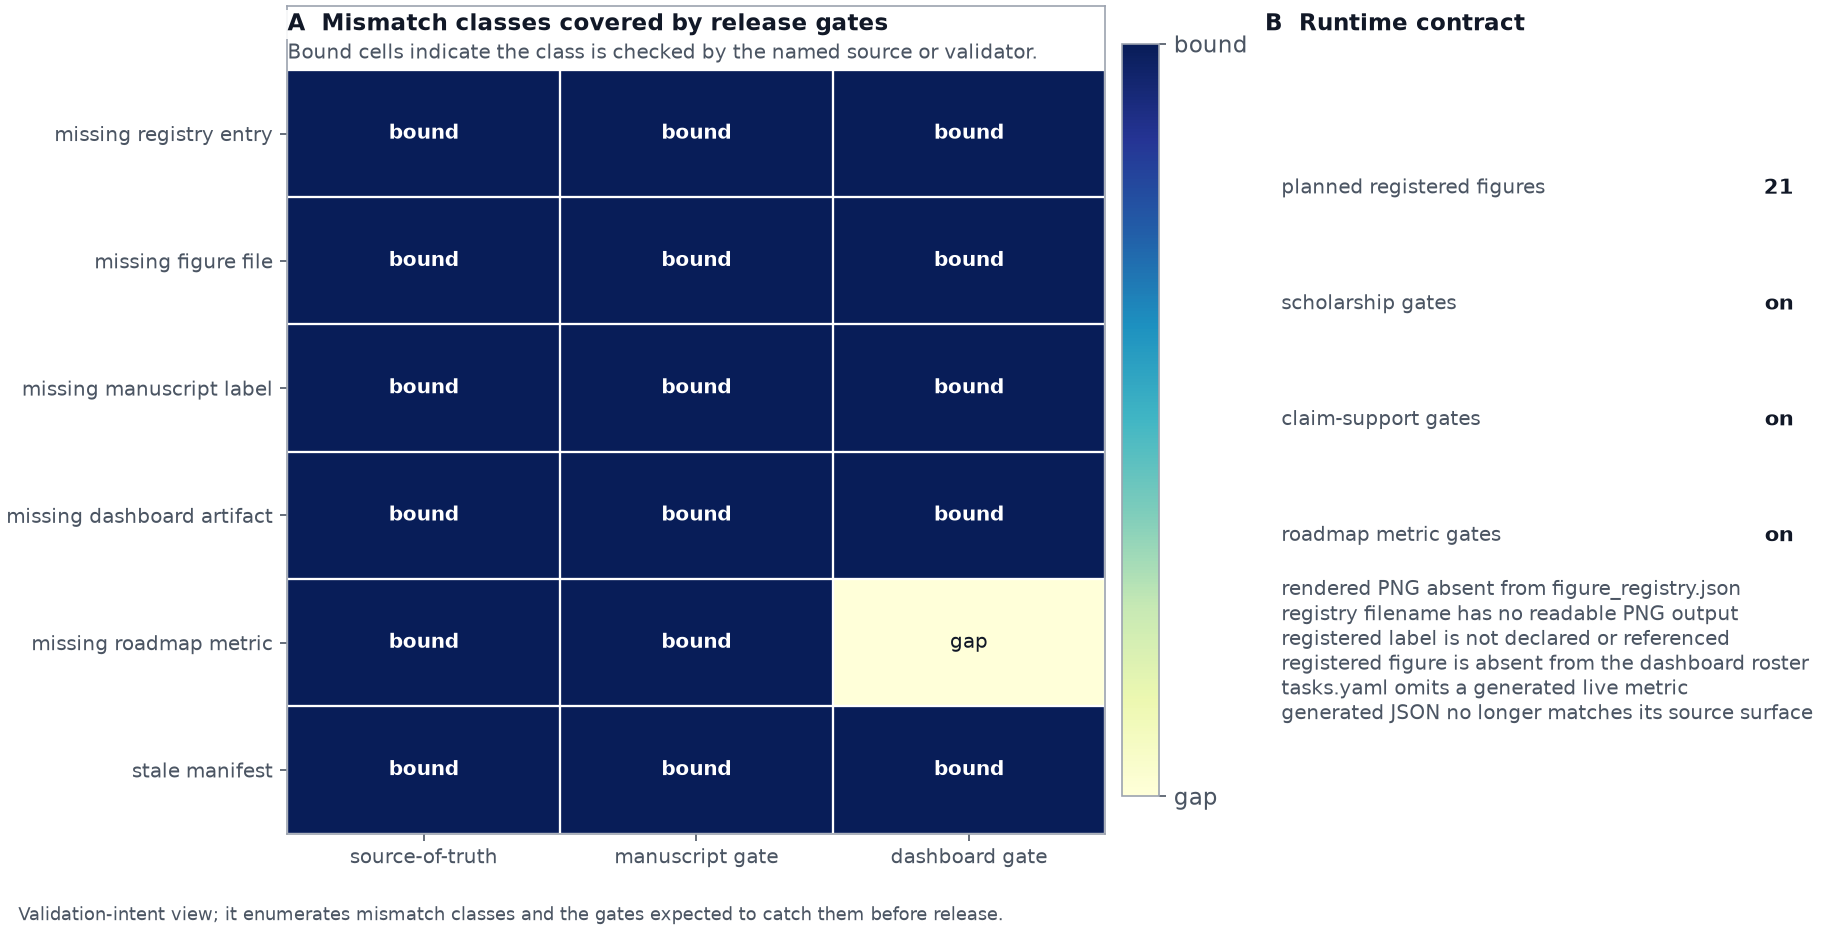
\includegraphics[width=0.98\linewidth,height=0.5\textheight,keepaspectratio,alt={Validation-intent mismatch matrix for Active Skillference. Rows enumerate concrete false-certification classes: a rendered PNG omitted from the registry, a registered figure without a readable file, a registered label omitted from the manuscript, a registered figure omitted from the dashboard artifact roster, a missing roadmap live metric, and a stale generated manifest. Columns show whether the source-of-truth, manuscript gate, or dashboard gate is expected to reject each mismatch before release. The right panel records the planned registered-figure count and which optional audit surfaces were enabled for the render.}]{../figures/validation_intent_mismatch_matrix.png}
\caption{Validation-intent mismatch matrix for Active Skillference. Rows
enumerate concrete false-certification classes: a rendered PNG omitted
from the registry, a registered figure without a readable file, a
registered label omitted from the manuscript, a registered figure
omitted from the dashboard artifact roster, a missing roadmap live
metric, and a stale generated manifest. Columns show whether the
source-of-truth, manuscript gate, or dashboard gate is expected to
reject each mismatch before release. The right panel records the planned
registered-figure count and which optional audit surfaces were enabled
for the render.}\label{fig:validation_intent_mismatch_matrix}
\end{figure}

The same contract is now represented inside the curriculum rather than
only enforced at release time. The visual-evidence slice adds a
prerequisite-gated authoring path for question contracts, data grain,
encoding strength, annotation boundaries, static/mobile readability, and
negative-control validation.
fig.~\ref{fig:visual_evidence_contract_ladder} shows that path as
generated curriculum evidence: each rung names the live skill that
carries the review step, while the registry and dashboard expose the
same structured chart-contract fields. This is a deterministic
artifact-integrity claim, not a claim that the visual curriculum has
been externally tested with learners.

\begin{figure}
\centering
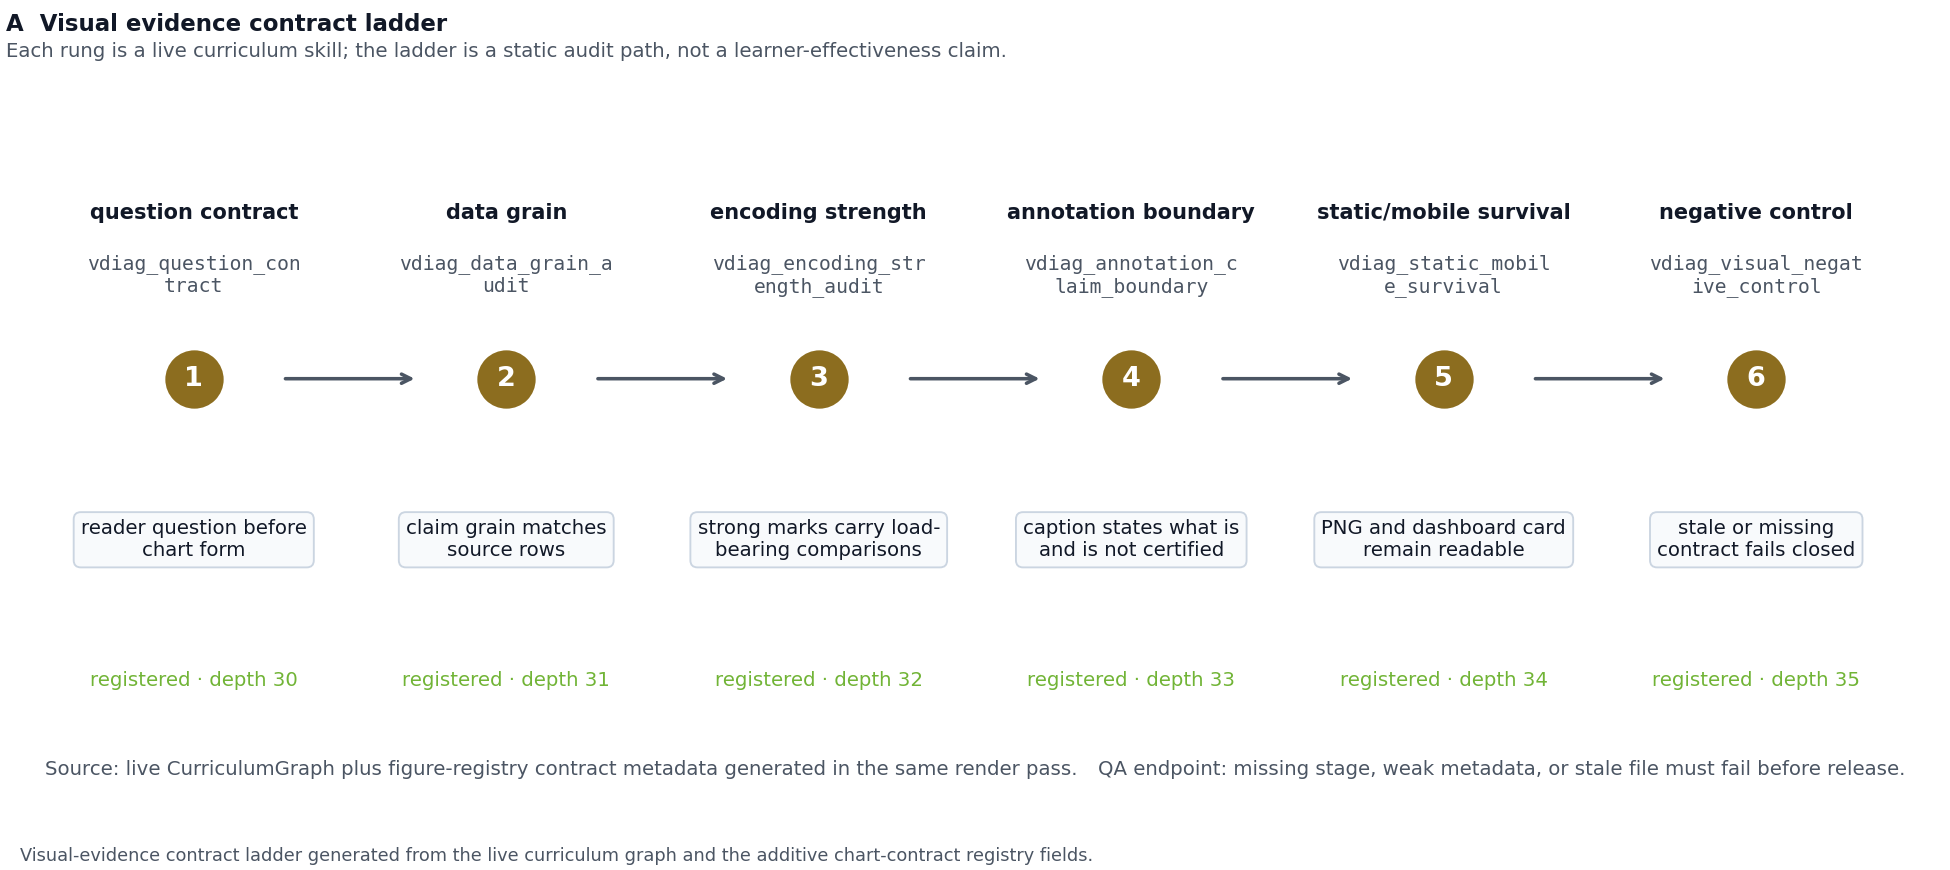
\includegraphics[width=0.98\linewidth,height=0.5\textheight,keepaspectratio,alt={Visual-evidence contract ladder generated from the live curriculum graph and figure registry metadata. Six numbered rungs move from question contract through data grain, encoding strength, annotation boundary, static/mobile survival, and negative-control validation. Each rung names the skill identifier that carries the review obligation and reports whether the skill is registered in the graph. The figure documents the authoring and validation lifecycle for visual evidence; it does not claim learner effectiveness or external deployment performance.}]{../figures/visual_evidence_contract_ladder.png}
\caption{Visual-evidence contract ladder generated from the live
curriculum graph and figure registry metadata. Six numbered rungs move
from question contract through data grain, encoding strength, annotation
boundary, static/mobile survival, and negative-control validation. Each
rung names the skill identifier that carries the review obligation and
reports whether the skill is registered in the graph. The figure
documents the authoring and validation lifecycle for visual evidence; it
does not claim learner effectiveness or external deployment
performance.}\label{fig:visual_evidence_contract_ladder}
\end{figure}

The scientific-claim layer adds one more audit view.
fig.~\ref{fig:scientific_evidence_matrix} is generated from manuscript
\texttt{claim-support} anchors and the support matrix in
\breaktt{data/manuscript\_claim\_support.yaml}. Its rows separate
computed, descriptive-count, simulation, literature, scope-limit,
delivery and visual claims; its columns show whether each class is
backed by claim tokens, manuscript variables, citations, figures,
validators or limitation markers. This is not a statistical result. It
is a release integrity check that prevents strong scientific wording
from passing without a declared evidence class.

\begin{figure}
\centering
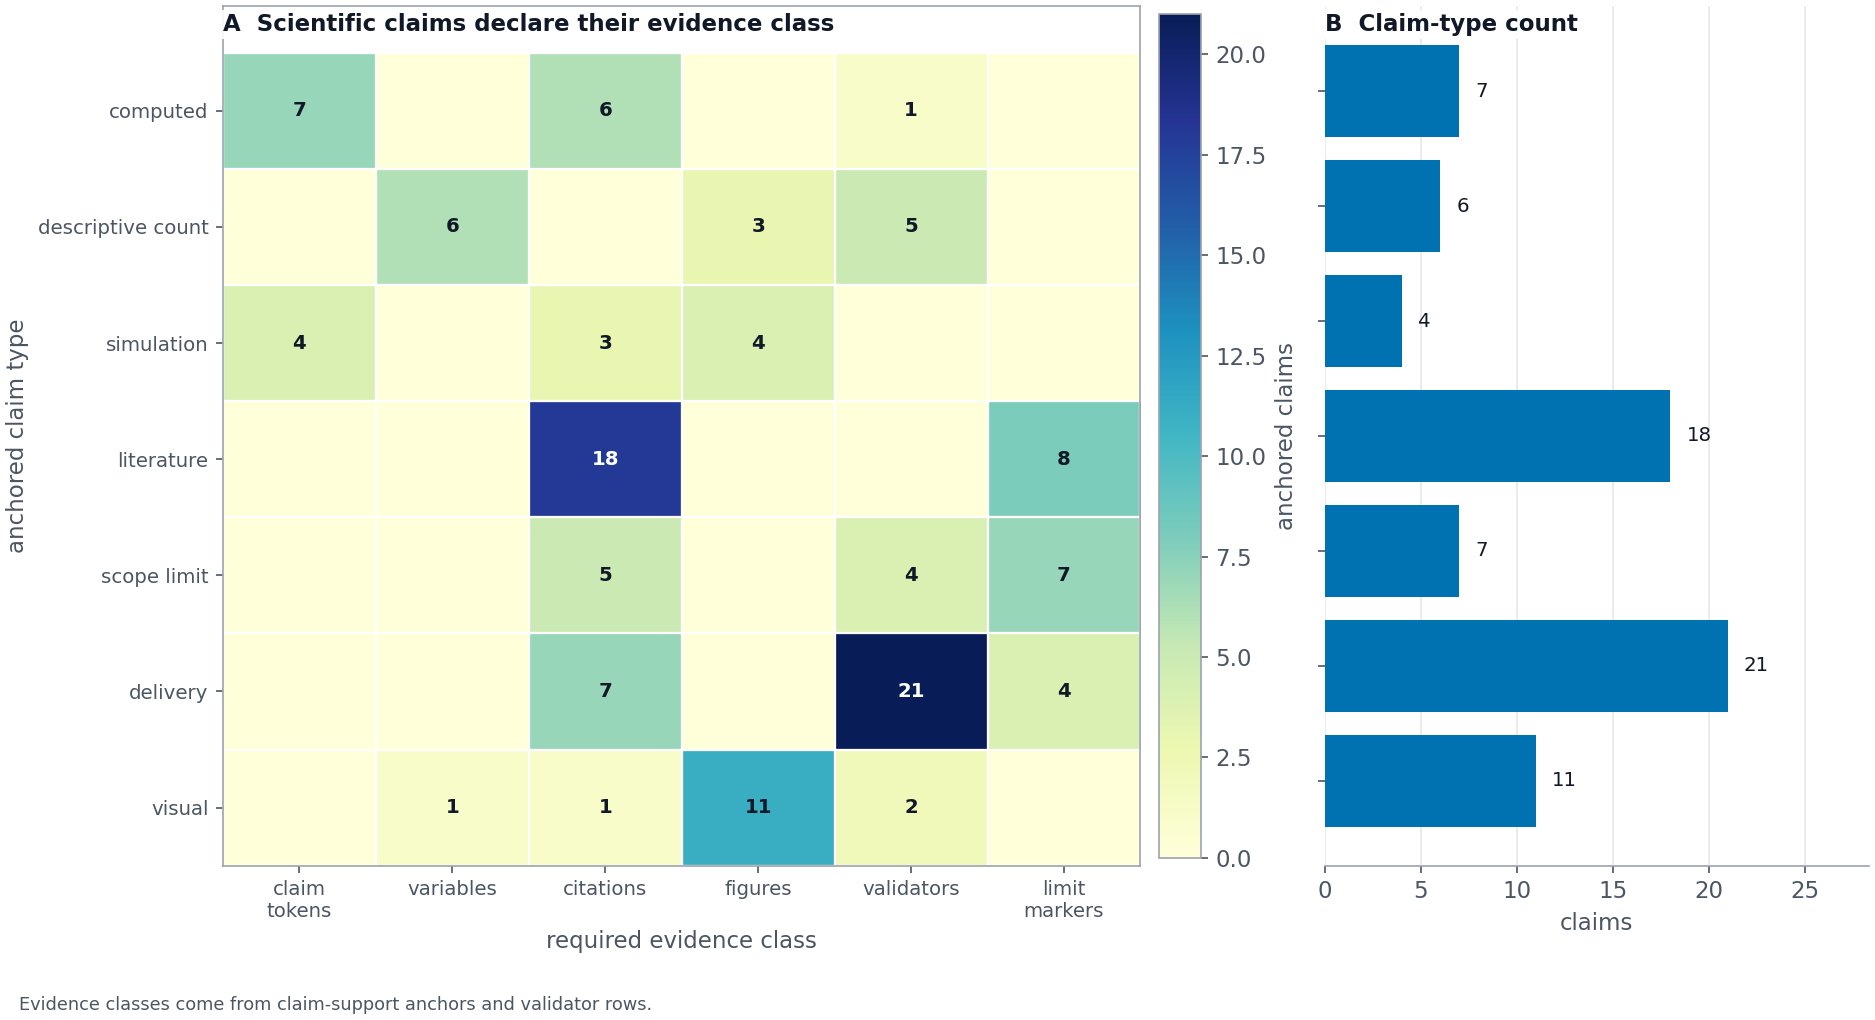
\includegraphics[width=0.96\linewidth,height=0.5\textheight,keepaspectratio,alt={Scientific evidence matrix for manuscript claims generated from claim-support anchors and data/manuscript\_claim\_support.yaml. Rows are claim-support types, columns are evidence classes, cell counts show how many anchored claims use each evidence class, and the side panel counts claims per type. The purpose is epistemic classification rather than statistical inference: computed, descriptive, simulation, literature, scope-limit, delivery, and visual claims are forced to declare the kind of support they actually have.}]{../figures/scientific_evidence_matrix.png}
\caption{Scientific evidence matrix for manuscript claims generated from
claim-support anchors and data/manuscript\_claim\_support.yaml. Rows are
claim-support types, columns are evidence classes, cell counts show how
many anchored claims use each evidence class, and the side panel counts
claims per type. The purpose is epistemic classification rather than
statistical inference: computed, descriptive, simulation, literature,
scope-limit, delivery, and visual claims are forced to declare the kind
of support they actually have.}\label{fig:scientific_evidence_matrix}
\end{figure}

The platform evidence above is intentionally separated from the small
mathematical examples. Those examples are still central teaching
artifacts, but their scientific meaning depends on the supplement's
model assumptions and regime boundaries.

\newpage

\section{Results: Kernel-Backed Teaching Examples and Model
Boundaries}\label{sec:results-kernel-examples}

\subsection{Kernel-generated mathematical examples and model
boundaries}\label{kernel-generated-mathematical-examples-and-model-boundaries}

The main result is not that this repository contains two illustrative
Active Inference plots; it is that the plots are generated from the same
kernel registry that binds the curriculum and manuscript. The
variational free-energy sweep fig.~\ref{fig:free_energy} and the
expected-free-energy policy comparison fig.~\ref{fig:efe} are therefore
treated as supplemental scientific walkthroughs rather than headline
platform evidence. They remain central teaching artifacts, but their
interpretation belongs with the derivation, model assumptions, and
regime boundaries in the supplement. This separation keeps Results
focused on what the platform demonstrates: structure, provenance,
scholarship, artifact wiring, and SkillTree handoff all regenerate
together.

The final result is delivery: the same validator-backed artifact that
supports the paper also becomes the SkillTree import payload and
dashboard inspection surface.

\newpage

\section{Results: SkillTree Export and Learner-Surface
Handoff}\label{sec:results-skilltree-dashboard-front-matter}

\subsection{SkillTree export, learner-surface handoff, and generated
front
matter}\label{skilltree-export-learner-surface-handoff-and-generated-front-matter}

All registered claims are produced by tested kernels; every claim token
in the 630 skills resolves, and the bare-number linter reports zero
violations across descriptions, assessment prompts, and correct numeric
answer options. The scholarship audit similarly resolves every authored
citation against the bibliography and source-role matrix. The
provenance-rendered graph exports to a SkillTree project of 111
subjects, 630 skills, 1199 learning-path dependencies, 630 quizzes, and
2520 assessment questions, with no unresolved tokens in the output. The
source reaches the configured \texttt{src/} coverage gate with no mocks;
exact current coverage is reported by the test run rather than asserted
in prose.

The dashboard delivery surface exposes the same contract. Its status
payload cross-checks SkillTree export counts against build stats, tracks
the claim ledger and figure artifacts, exposes the manuscript artifact
audit, mounts the official learner display when SkillTree is online, and
gives each skill a direct handoff into that display's subject and
quiz-gated skill pages. This avoids the common false demo in which a
polished local UI merely copies course text: the local page can inspect
and preview artifacts, but the learning and quiz actions are routed to
the seeded SkillTree project.

Prose cannot settle that distinction, so the delivery surface is also
recorded directly. fig.~\ref{fig:app_operational_snapshot} shows the
landing view reporting exported counts, live SkillTree dependency
parity, and artifact presence together.
fig.~\ref{fig:app_official_learner_view} shows SkillTree's own client
library rendering the seeded project inside the local page, with its
native points, level, progress rings, and ranking; that is the
observation the export-lands-in-the-platform reading needs, and no
exported JSON file can supply it.
fig.~\ref{fig:app_curriculum_learn_material} shows the generated lesson
record for one skill beside its commit-pinned upstream pointers, so the
material boundary is visible rather than asserted.
fig.~\ref{fig:app_dependency_graph} shows the captioned
prerequisite-flow table that carries the heaviest subject-to-subject
relations for readers who cannot use the lane drawing, which is a ranked
summary of that structure rather than a complete substitute for every
edge, and fig.~\ref{fig:app_runtime_deployment_matrix} shows
deployment-mode readiness beside the browser-visible runtime payload,
where the admin password and client secret are absent. These five images
are recordings rather than renders: unlike every other figure here they
cannot be rebuilt from project data, so they are version-controlled,
marked in the figure registry as captured evidence, and stamped with the
dashboard URL, viewport, live counts, capture timestamp, per-image
digest, and full-stack mode of the run that produced them. Being
recordings, they are also the one family exempt from the check that
every registered figure was emitted by the render pipeline; the
exemption is recorded in the registry rather than left implicit, and
their integrity rests on the digest and provenance record instead.

The front matter follows the same rule. The cover image is generated
from the live graph, claim registry and roadmap metrics, and the
page-two named-skill atlas is generated from every authored skill name
in the curriculum graph. Both images are checked by publication-asset
audits before rendering. The cover uses a square layout so it can serve
both PDF title-page and web artifact contexts; the atlas uses a wide
page-two layout so the skill-name vocabulary remains readable by showing
a reduced weighted-term sample and representative dependency checkpoints
rather than a complete printed index. Neither asset is a numbered
scientific figure: the dashboard exposes them as cover-category
artifacts, while \breaktt{figure\_registry.json} remains reserved for
manuscript figures that are declared and cross-referenced in the text.
This prevents polished front matter from becoming a false-certification
path outside the artifact contract.

\begin{figure}
\centering
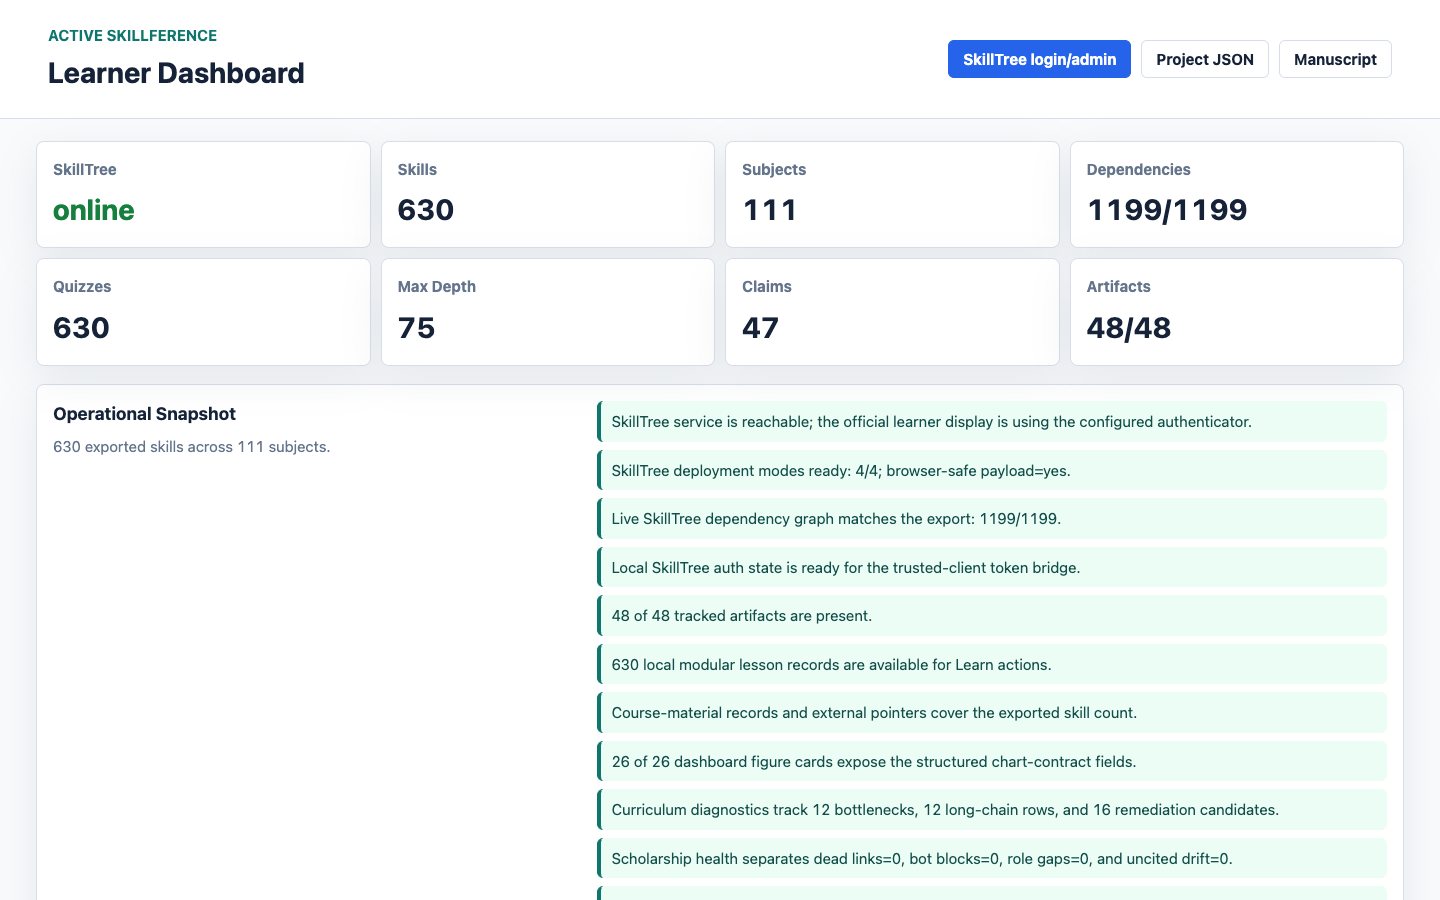
\includegraphics[width=1\linewidth,height=0.5\textheight,keepaspectratio,alt={Learner dashboard landing view captured from the running local stack. The metric row reports exported skills, subjects, quizzes, maximum prerequisite depth, registered claims, and artifact presence, while the dependency metric shows live SkillTree parity against the export rather than the exported count alone. The evidence list below restates those machine-checked conditions in words: export counts, live graph parity, local auth readiness, course-material coverage, and figure-contract completeness are surfaced together on one page instead of being scattered across separate reports. The list continues past the fold; the frame shows the first ten of its rows. The artifact tally counts this evidence family among the tracked artifacts, so it is a completeness check on the roster rather than an independent audit of these images.}]{../figures/app_operational_snapshot.png}
\caption{Learner dashboard landing view captured from the running local
stack. The metric row reports exported skills, subjects, quizzes,
maximum prerequisite depth, registered claims, and artifact presence,
while the dependency metric shows live SkillTree parity against the
export rather than the exported count alone. The evidence list below
restates those machine-checked conditions in words: export counts, live
graph parity, local auth readiness, course-material coverage, and
figure-contract completeness are surfaced together on one page instead
of being scattered across separate reports. The list continues past the
fold; the frame shows the first ten of its rows. The artifact tally
counts this evidence family among the tracked artifacts, so it is a
completeness check on the roster rather than an independent audit of
these images.}\label{fig:app_operational_snapshot}
\end{figure}

\begin{figure}
\centering
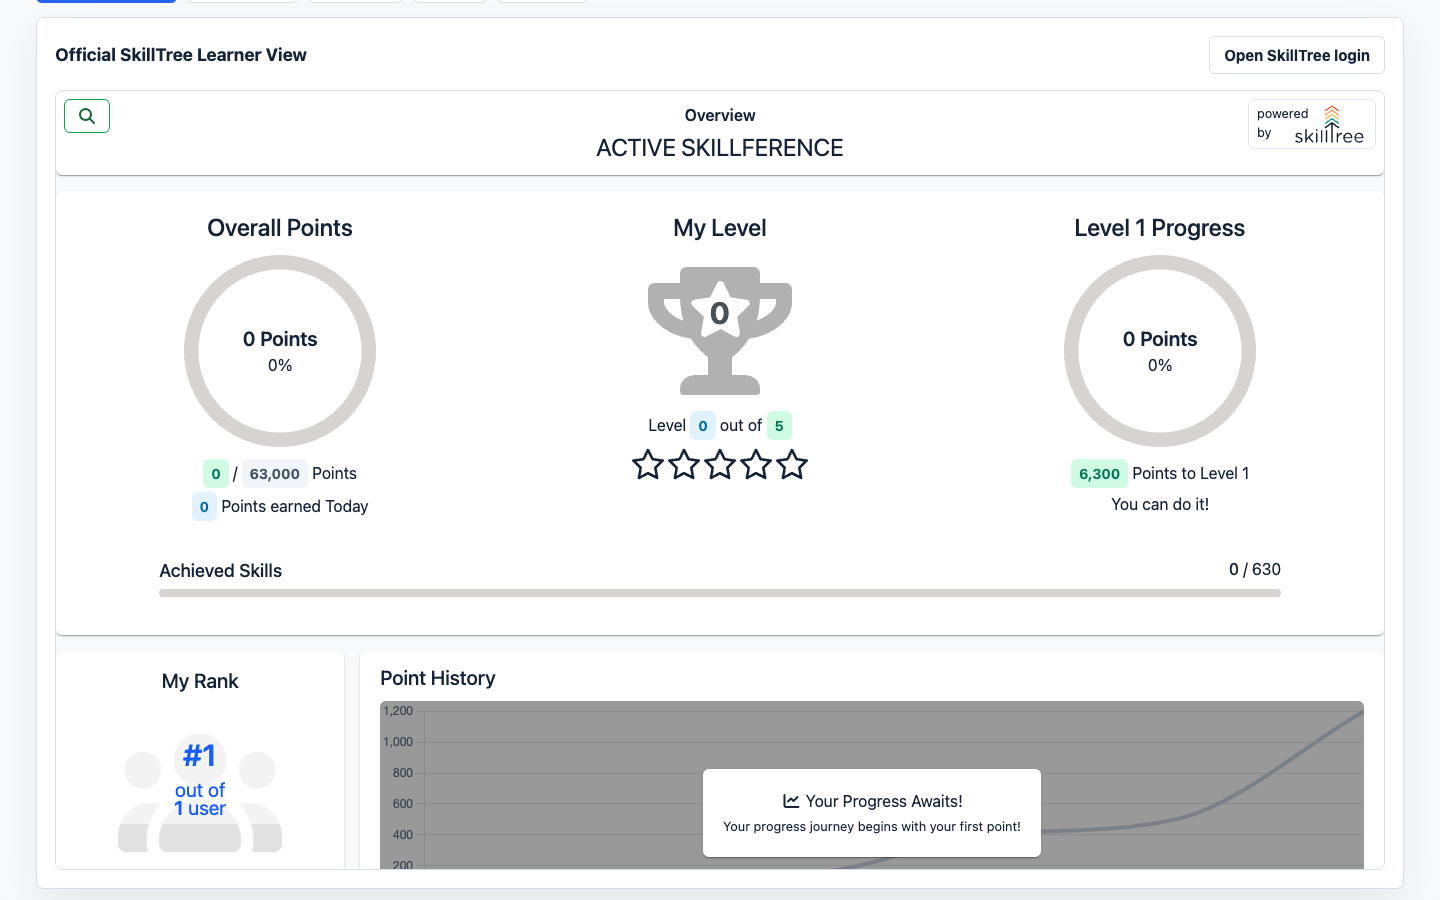
\includegraphics[width=1\linewidth,height=0.5\textheight,keepaspectratio,alt={The Official Display tab captured while the embedded SkillTree learner client is mounted against the seeded project. The overview header, overall points, level and level progress rings, the achieved-skills bar reading zero of the full exported skill count, the personal rank card, and the point-history panel are all rendered by SkillTree's own client library inside the project dashboard, which is the demonstration that the export lands in the platform runtime rather than in a project reimplementation of it. Every progress value reads zero and the point-history panel shows its first-point empty state, because the capture uses a freshly seeded local identity that has completed nothing.}]{../figures/app_official_learner_view.png}
\caption{The Official Display tab captured while the embedded SkillTree
learner client is mounted against the seeded project. The overview
header, overall points, level and level progress rings, the
achieved-skills bar reading zero of the full exported skill count, the
personal rank card, and the point-history panel are all rendered by
SkillTree's own client library inside the project dashboard, which is
the demonstration that the export lands in the platform runtime rather
than in a project reimplementation of it. Every progress value reads
zero and the point-history panel shows its first-point empty state,
because the capture uses a freshly seeded local identity that has
completed nothing.}\label{fig:app_official_learner_view}
\end{figure}

\begin{figure}
\centering
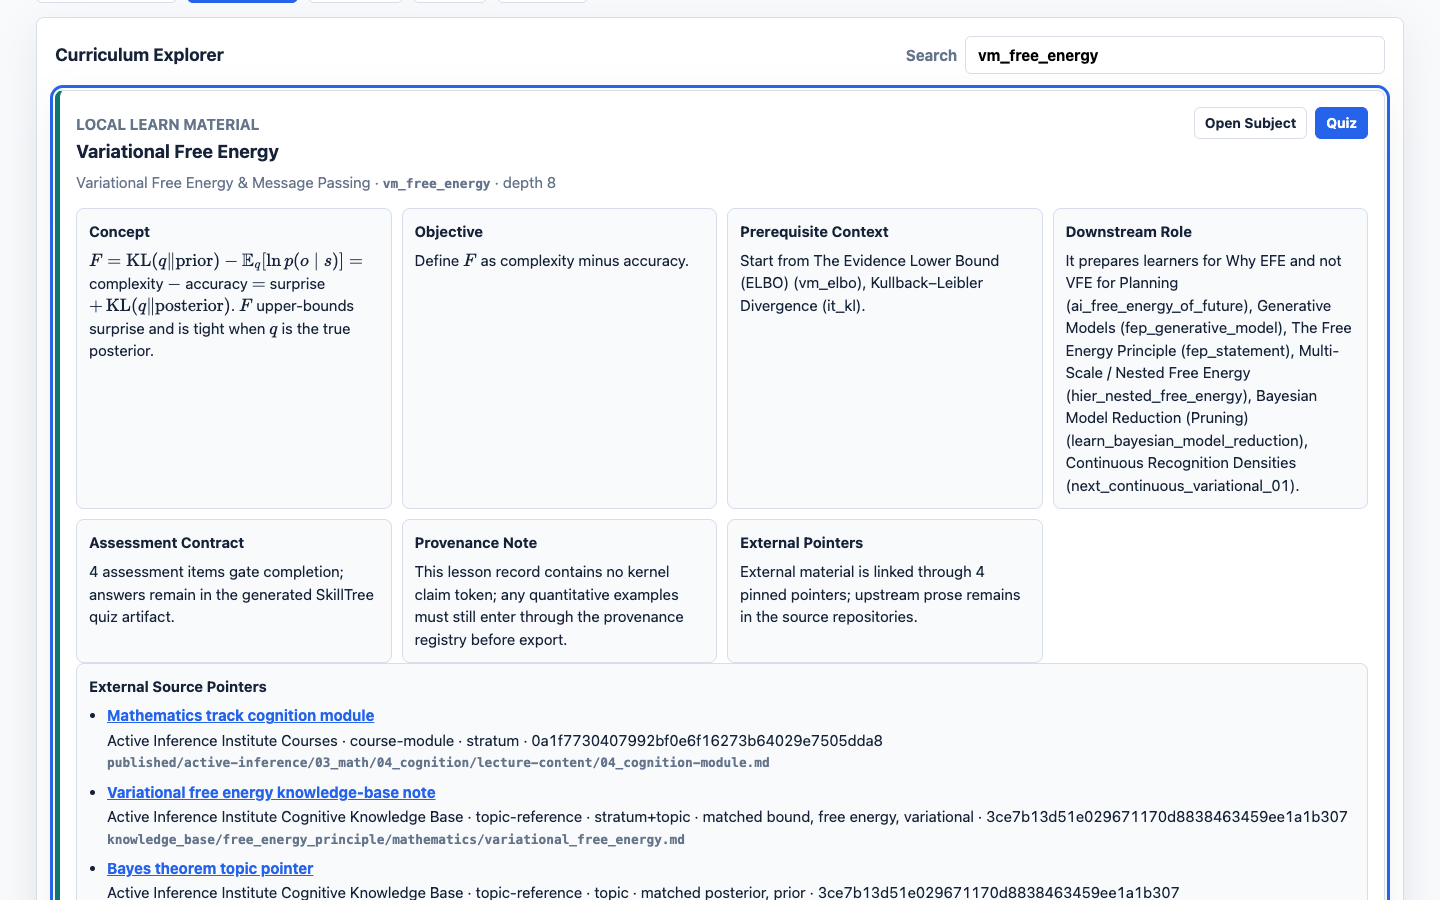
\includegraphics[width=1\linewidth,height=0.5\textheight,keepaspectratio,alt={The Curriculum tab captured with the generated lesson record for the variational free energy skill opened through its Learn action. The panel shows the concept context, prerequisite position, downstream role, assessment summary, and the commit-pinned external source pointers generated for that skill, alongside the handoff buttons that return the learner to the official SkillTree subject and quiz routes. It is the delivery counterpart to the course-material provenance rule: local lessons link out to pinned upstream sources instead of copying them.}]{../figures/app_curriculum_learn_material.png}
\caption{The Curriculum tab captured with the generated lesson record
for the variational free energy skill opened through its Learn action.
The panel shows the concept context, prerequisite position, downstream
role, assessment summary, and the commit-pinned external source pointers
generated for that skill, alongside the handoff buttons that return the
learner to the official SkillTree subject and quiz routes. It is the
delivery counterpart to the course-material provenance rule: local
lessons link out to pinned upstream sources instead of copying
them.}\label{fig:app_curriculum_learn_material}
\end{figure}

\begin{figure}
\centering
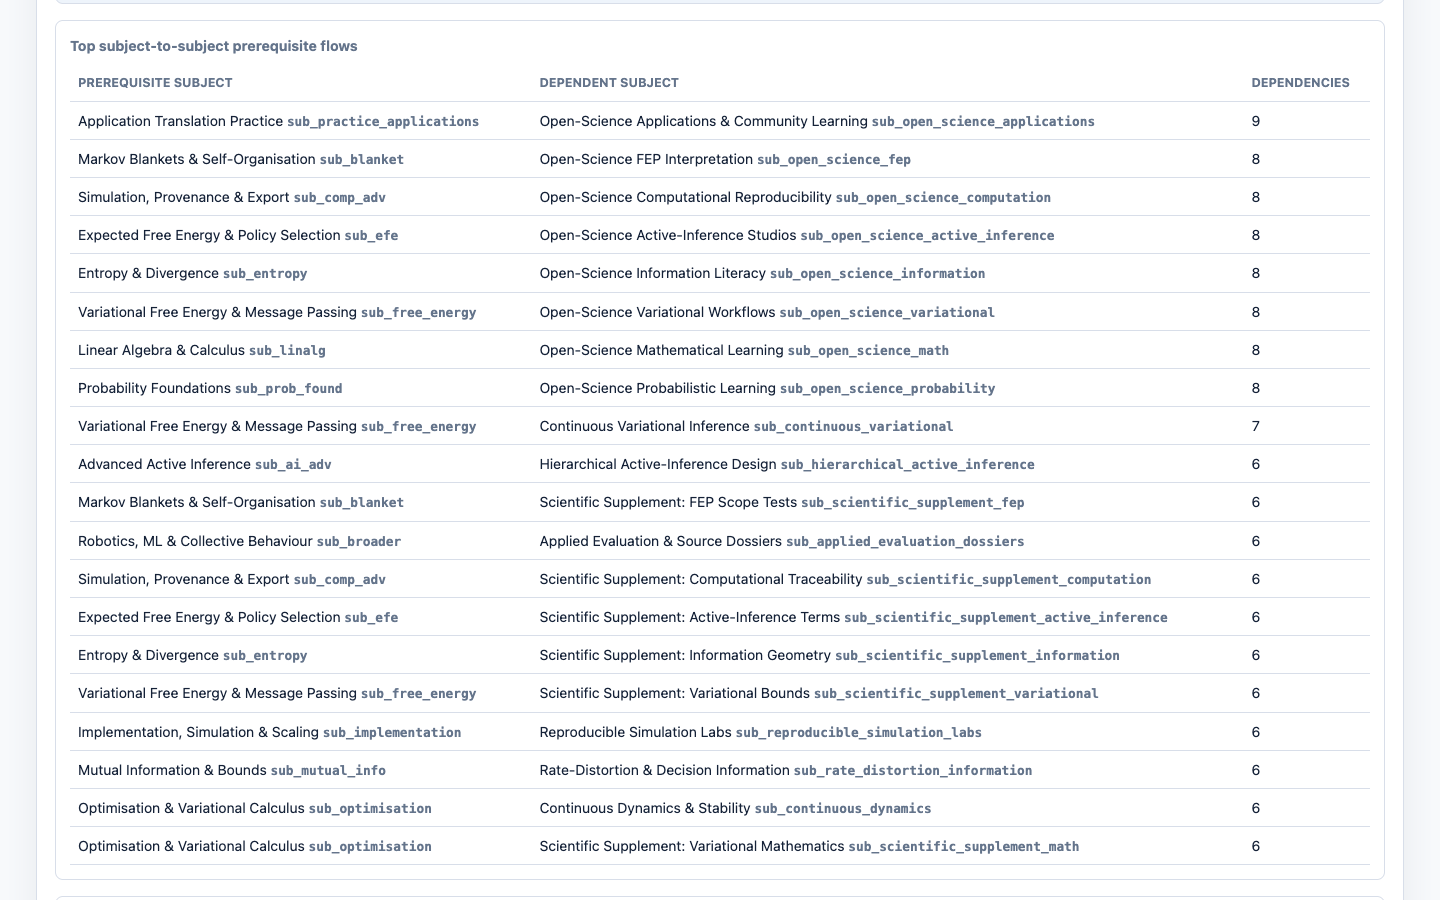
\includegraphics[width=1\linewidth,height=0.5\textheight,keepaspectratio,alt={The accessible prerequisite-flow table in the Graph tab, scrolled past the subject lane canvas that sits above it in the same panel. Table and canvas are built from the same server-computed flow summaries, so the prerequisite structure reaches a keyboard or screen-reader user as captioned rows with real header cells rather than only as a drawing. Each row is one directed subject-to-subject relation: a prerequisite subject, the dependent subject that requires it, and how many skill dependencies run between them, ordered by weight.}]{../figures/app_dependency_graph.png}
\caption{The accessible prerequisite-flow table in the Graph tab,
scrolled past the subject lane canvas that sits above it in the same
panel. Table and canvas are built from the same server-computed flow
summaries, so the prerequisite structure reaches a keyboard or
screen-reader user as captioned rows with real header cells rather than
only as a drawing. Each row is one directed subject-to-subject relation:
a prerequisite subject, the dependent subject that requires it, and how
many skill dependencies run between them, ordered by
weight.}\label{fig:app_dependency_graph}
\end{figure}

\begin{figure}
\centering
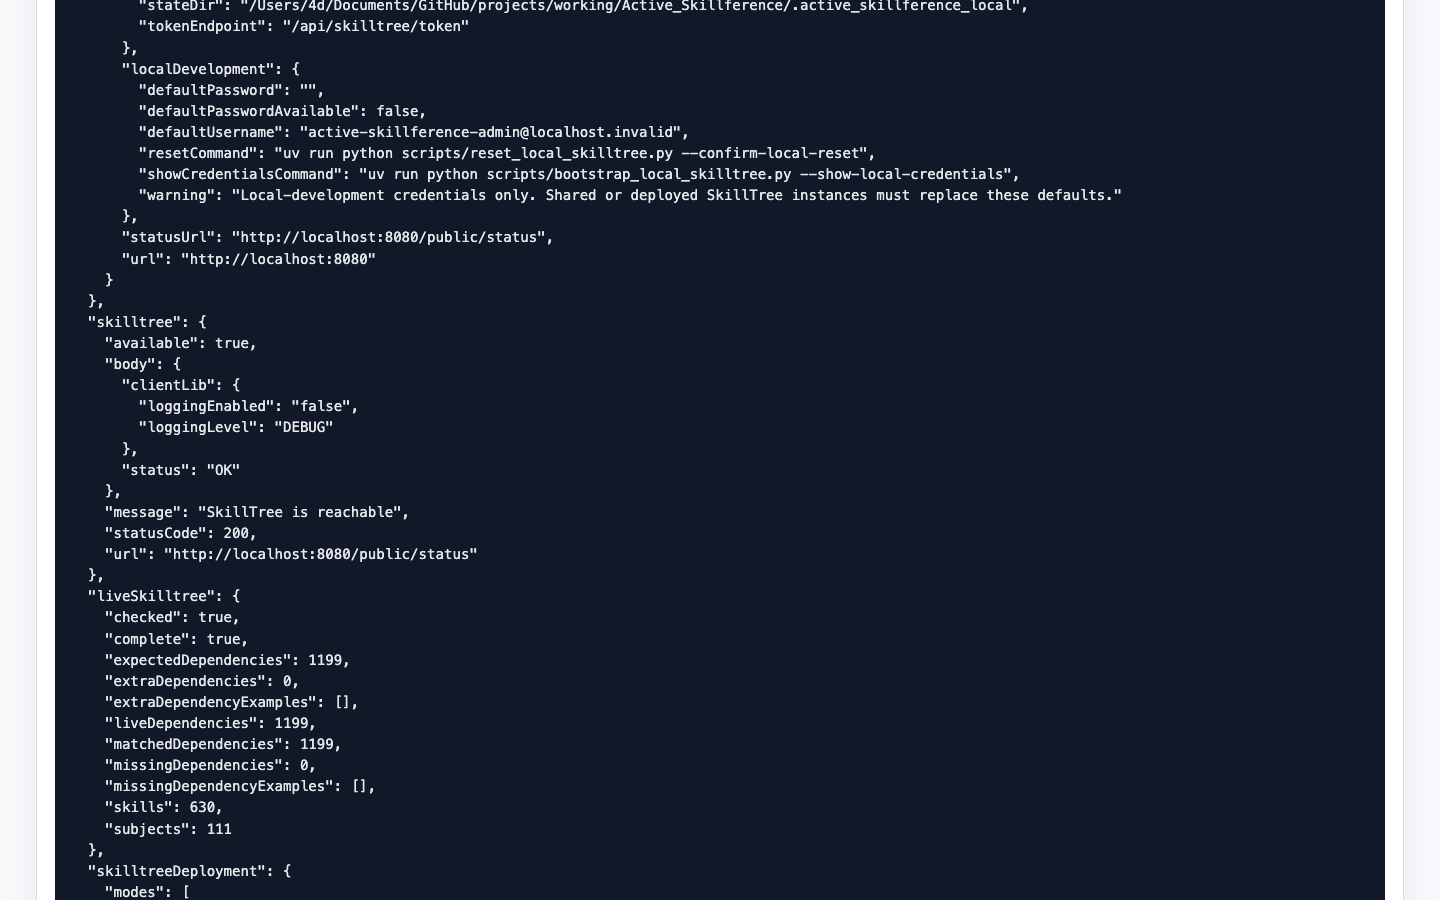
\includegraphics[width=1\linewidth,height=0.5\textheight,keepaspectratio,alt={The browser-visible runtime payload in the Runtime tab, scrolled past the deployment-mode matrix to the local development block. The default password field is an empty string and its availability flag is false, so the page reports the local username and the recovery commands while withholding the credential itself; no client secret and no bearer token appear anywhere in the payload. The same view carries the SkillTree reachability block and the live dependency parity block reporting complete parity with no missing or extra edges, which is the auth-boundary evidence in the form the browser actually receives it.}]{../figures/app_runtime_deployment_matrix.png}
\caption{The browser-visible runtime payload in the Runtime tab,
scrolled past the deployment-mode matrix to the local development block.
The default password field is an empty string and its availability flag
is false, so the page reports the local username and the recovery
commands while withholding the credential itself; no client secret and
no bearer token appear anywhere in the payload. The same view carries
the SkillTree reachability block and the live dependency parity block
reporting complete parity with no missing or extra edges, which is the
auth-boundary evidence in the form the browser actually receives
it.}\label{fig:app_runtime_deployment_matrix}
\end{figure}

\newpage

\section{Discussion and Conclusion: What the Artifact Establishes---and
What It Does
Not}\label{discussion-and-conclusion-what-the-artifact-establishesand-what-it-does-not}

\subsection{Principal findings: a claim-calibrated curriculum
artifact}\label{principal-findings-a-claim-calibrated-curriculum-artifact}

Active Skillference establishes a bounded engineering result: a
contested formal subject can be represented as an inspectable
prerequisite graph whose structural, quantitative, scholarly, and
delivery contracts are checked separately. The curriculum graph is a
validated DAG; learner-facing computed values are resolved from tested
kernels; citations are assigned source roles; and generated figures,
manuscript references, and SkillTree payloads are audited as connected
artifacts. These are properties of this checkout and its build process,
not evidence that the selected order is optimal for every learner or
that the underlying scientific framework is empirically confirmed.

\subsection{Interpretation: infrastructure rather than intelligence or
personalization}\label{interpretation-infrastructure-rather-than-intelligence-or-personalization}

The mathematical examples and the curriculum infrastructure operate at
different levels. The kernels implement small, model-dependent
demonstrations of inference and policy evaluation. The curriculum layer
orders and assesses concepts. The provenance layer records how values
and sources enter the learner-facing artifact. None of these layers is
an intelligent tutor, a general-purpose reasoning system, or an adaptive
learner model. In particular, the term \emph{agent} in the mathematical
examples refers to a formal model with specified states, observations,
preferences, and policies; it should not be read as a claim about
consciousness, general intelligence, autonomy, or human-like learning.

The related-work literature supports this separation. Active Inference
formulations can connect belief updating, action selection, learning,
and epistemic behavior, but their predictions depend on the generative
model, preferences, approximation, and policy set
\citep{rao1999predictive, friston2013life, ramstead2018answering, friston2019particular}.
The supplement therefore keeps the VFE/EFE derivations, sign
conventions, and preference assumptions visible instead of treating one
computed policy comparison as a universal account of intelligent
behavior. Learner-state models such as knowledge tracing and Q-matrix
cognitive diagnosis belong to a separate adaptive-learning evidence
layer and are cited here as comparison boundaries, not as components of
this artifact
\citep{piech2015deep_knowledge_tracing, tao2024q_matrix_constraint}.

\subsection{Implications: future adaptive learning systems and
open-science
interoperability}\label{implications-future-adaptive-learning-systems-and-open-science-interoperability}

The delivery contract is useful precisely because it does not hide
ownership boundaries. The exporter creates a SkillTree-compatible
Project -\textgreater{} Subject -\textgreater{} Skill profile with
learning-path dependencies and quiz associations. The local dashboard
exposes generated artifacts and opens official subject and quiz routes,
while SkillTree remains the owner of progress, ranking, scoring,
completion, and authentication. This makes the repository a candidate
foundation for a later adaptive study, not an adaptive system in the
present release.

A genuinely adaptive extension would require learner response data, a
validated model of learner state, a transparent rule for selecting the
next skill, item-level measurement, privacy and consent controls, and
prospective evaluation against a preregistered comparator
\citep{doignon1985knowledge_spaces, fu2025curriculum_aware_gncd, designbasedresearchcollective2003, liu2023_learning_analytics_privacy, piech2015deep_knowledge_tracing, tao2024q_matrix_constraint}.
Knowledge tracing and Q-matrix cognitive diagnosis are comparison
literatures for those stronger commitments, not components of the
present export. Provenance and graph validation would remain necessary
infrastructure, but they would not by themselves establish
personalization quality or learning effectiveness.

The community contribution should be read at the same bounded level. The
Active Inference Institute's public website repository presents a public
resource hub for learning, research, participation, and contribution,
with public repositories and a documented boundary between internal
inputs and verified public projections
\citep{activeinferenceinstitute2026website}. Active Skillference
contributes a complementary artifact to that open-science environment:
it packages a prerequisite graph, kernel-backed examples, source-role
audit, and SkillTree handoff into a rerunnable educational release. The
relationship is interoperable and community-facing, not institutional:
this repository does not claim to be an Institute product, an official
curriculum, or an endorsement of any contributor or public pathway.

\subsection{Limitations and planned empirical
evaluation}\label{limitations-and-planned-empirical-evaluation}

The release state is machine-readable. As of 2026-07-31,
\texttt{tasks.yaml} records 78 roadmap tasks: 74 completed milestones
and 4 open items across metadata, skilltree, validation.
\texttt{TODO.md} is rendered from the same source.
fig.~\ref{fig:roadmap_risk} shows the current distribution of open
versus completed work by surface and release class, keeping
release-readiness language tied to the validator state that drives the
roadmap.

\begin{figure}
\centering
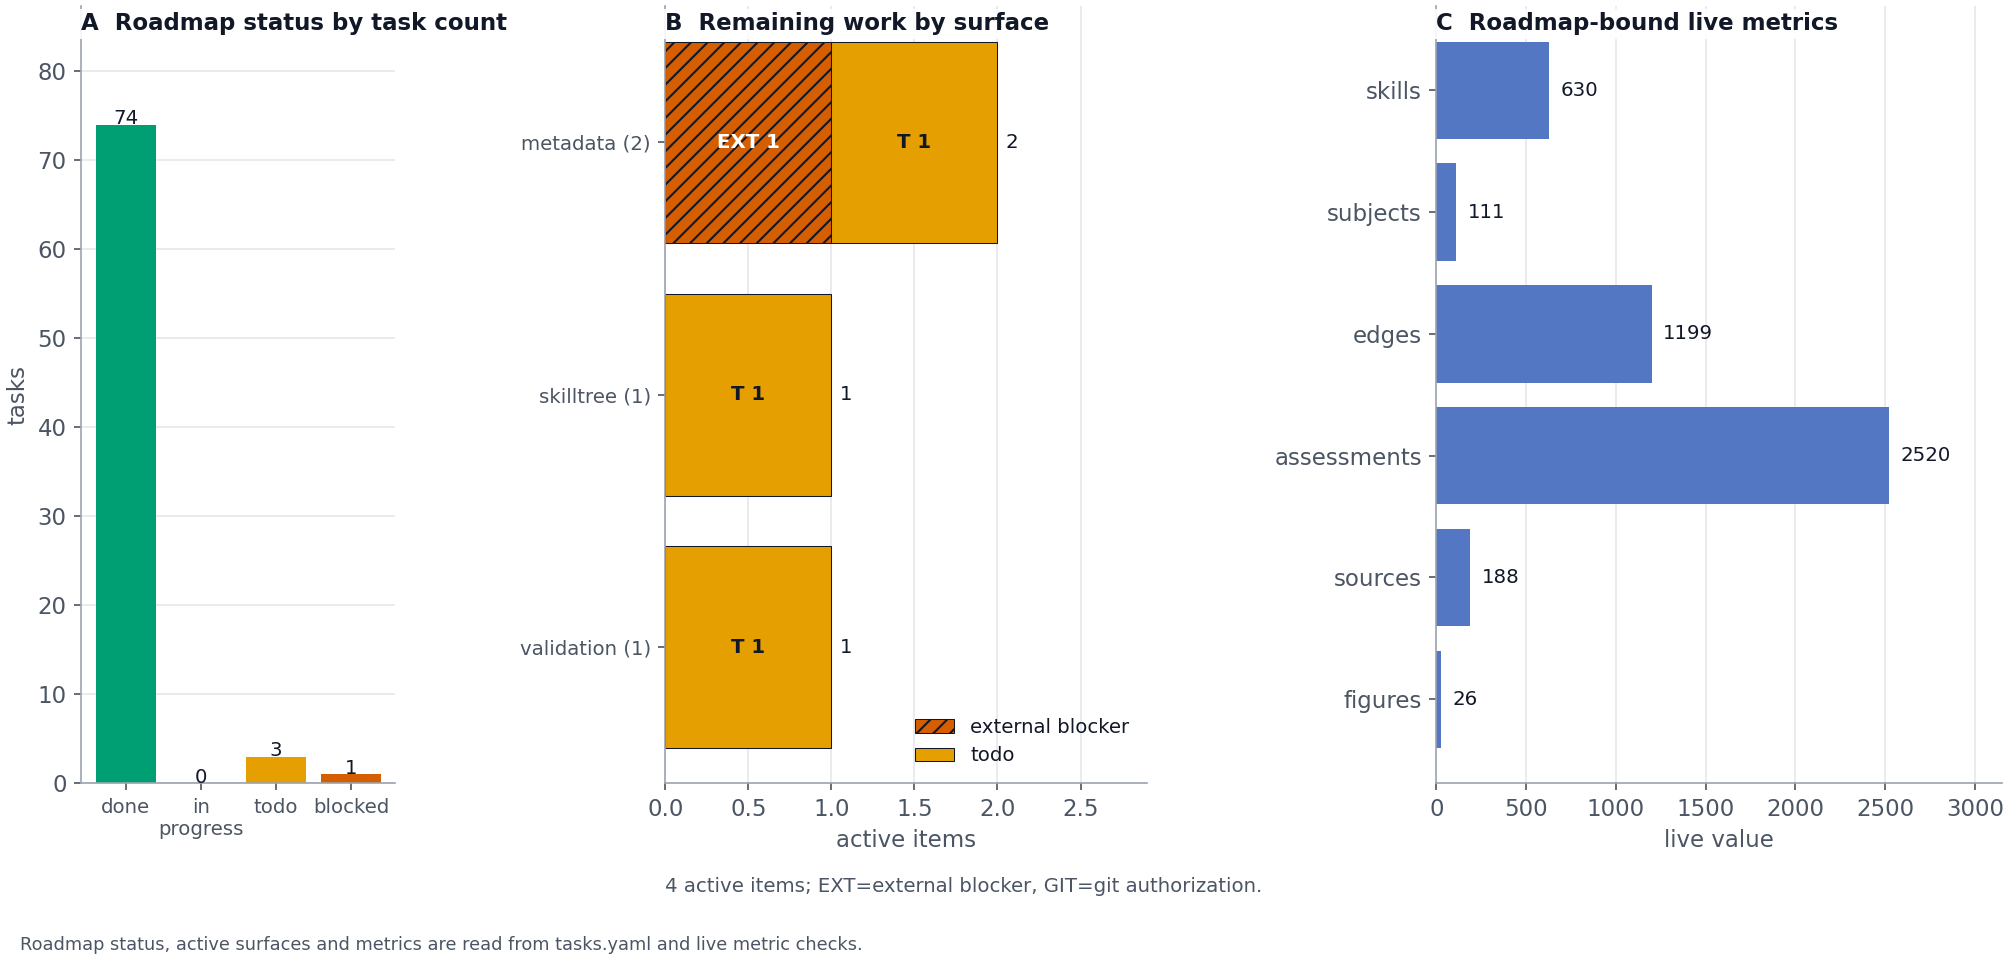
\includegraphics[width=0.88\linewidth,height=0.5\textheight,keepaspectratio,alt={Roadmap status by artifact surface generated from tasks.yaml and the live metrics stored in the roadmap source data. The first panel counts roadmap items by status, the middle panel groups remaining open or blocked work by surface and release class with direct EXT/GIT segment labels, hatching, and surface totals, and the final panel reports current curriculum, assessment, scholarship, and figure metrics. The figure separates external blockers from git-authorization hygiene using machine-readable roadmap data, so release-readiness text must agree with the same source.}]{../figures/roadmap_risk.png}
\caption{Roadmap status by artifact surface generated from
\protect\texttt{tasks.yaml} and the live metrics stored in the roadmap
source data. The first panel counts roadmap items by status, the middle
panel groups remaining open or blocked work by surface and release class
with direct EXT/GIT segment labels, hatching, and surface totals, and
the final panel reports current curriculum, assessment, scholarship, and
figure metrics. The figure separates external blockers from
git-authorization hygiene using machine-readable roadmap data, so
release-readiness text must agree with the same
source.}\label{fig:roadmap_risk}
\end{figure}

The limitations are therefore substantive rather than cosmetic. The
kernels cover fixed, small discrete teaching cases and bounded
predictive-coding or planning demonstrations; their conclusions depend
on the stated model, preferences, inputs, and approximation regime. The
runtime depends on SkillTree for live progress and quiz state, and this
release contains no learner-response data, learner-state inference,
retention measure, transfer measure, efficacy estimate, or
differential-benefit analysis. The planned pilot described in
sec.~\ref{sec:evaluation-setup-deterministic-tests-learner-study} and
the fuller boundary analysis in
sec.~\ref{sec:limitations-delivery-dependencies-learner-outcomes} define
the evidence needed before those claims can be made.

\subsection{Conclusion: a bounded, reproducible
contribution}\label{conclusion-a-bounded-reproducible-contribution}

The strongest conclusion is narrower and more useful: Active
Skillference makes the construction, provenance, and delivery of a
formal Active Inference curriculum more inspectable, reproducible, and
auditable. It establishes an infrastructure artifact and an
open-science-compatible handoff surface; it does not establish
intelligent tutoring, personalization, learner improvement, or empirical
confirmation of the Free Energy Principle.

\newpage

\section{Evaluation Setup: Deterministic Artifact Tests and Planned
Learner
Study}\label{sec:evaluation-setup-deterministic-tests-learner-study}

\subsection{Deterministic model suite and fixed
inputs}\label{deterministic-model-suite-and-fixed-inputs}

All quantitative results derive from small, fully specified discrete
models evaluated by the kernels with a fixed seed (\texttt{20260609}).
Within the supported Python, NumPy and Matplotlib environment, the model
inputs and graph ordering are deterministic; this is a
software-environment reproducibility claim, not a cross-hardware bitwise
proof.

\begin{itemize}
\tightlist
\item
  \textbf{Noisy-sensor model} (Bayes and VFE results): two latent
  states, \texttt{present} and \texttt{absent}, with prior
  \(D=[0.01, 0.99]\) and likelihood rows \([0.99, 0.05]\) and
  \([0.01, 0.95]\) over \texttt{positive} and \texttt{negative}
  observations. These model parameters are registered as kernel claims,
  so the prose cannot drift from \breaktt{src/kernels/examples.py}. This
  model emits the posterior, evidence probability, negative
  log-evidence, and free-energy sweep.
\item
  \textbf{Informative-sensor model} (EFE decomposition): likelihood rows
  \([0.9, 0.1]\) and \([0.1, 0.9]\) with observation preference
  \(C=[0.9, 0.1]\). This isolates epistemic value under uncertain versus
  certain beliefs.
\item
  \textbf{Two-action agent}: a neutral-preference sample/commit model
  with prior \(D=[0.5,0.5]\). The \emph{sample} action preserves the
  uncertain belief; the \emph{commit} action collapses belief mass
  toward one state. A sensor-precision sweep over this same model
  identifies the sample/commit switch.
\item
  \textbf{Information examples}: a fair coin, a fair six-sided die, a
  biased \(0.9/0.1\) coin, a one-in-a-hundred event, and a correlated
  joint distribution with entries \([0.4,0.1,0.1,0.4]\).
\end{itemize}

\subsection{Curriculum export and runtime ownership
boundary}\label{curriculum-export-and-runtime-ownership-boundary}

The curriculum spans the eight strata declared in
\breaktt{manuscript/config.yaml}. The maximal-enumeration floor is 630
skills (achieved: 630), and the current catalog adds
practice-and-translation material across all strata. That material
specifies opportunities to rehearse model checking, debugging, policy
design, implementation review, and application evaluation; it does not
establish that learners will acquire those abilities. Skills default to
100 points, one occurrence to completion, and \texttt{Quiz}
self-reporting so completion is assessment-gated. SkillTree export
targets project id \texttt{activeInference}.

\subsection{Reproduction, delivery, and release
checks}\label{reproduction-delivery-and-release-checks}

The generation pipeline is deterministic and runs from the project root
with no Docker daemon and no browser. Only
\breaktt{validate\_course\_material\_sources.py\ -\/-online} leaves the
machine, and only to re-resolve the cited course-material sources:

\begin{Shaded}
\begin{Highlighting}[]
\ExtensionTok{uv}\NormalTok{ run python scripts/build\_curriculum.py   }\CommentTok{\# validate the DAG, emit stats}
\ExtensionTok{uv}\NormalTok{ run python scripts/run\_kernels.py        }\CommentTok{\# claims, scholarship, figures, artifact audit}
\ExtensionTok{uv}\NormalTok{ run python scripts/build\_course\_materials.py}
\ExtensionTok{uv}\NormalTok{ run python scripts/validate\_course\_material\_sources.py }\AttributeTok{{-}{-}online}
\ExtensionTok{uv}\NormalTok{ run python scripts/validate\_manuscript\_artifacts.py}
\ExtensionTok{uv}\NormalTok{ run python scripts/validate\_docker\_digests.py}
\ExtensionTok{uv}\NormalTok{ run python scripts/validate\_release\_readiness\_inventory.py}
\ExtensionTok{uv}\NormalTok{ run python scripts/export\_skilltree.py   }\CommentTok{\# provenance{-}gated SkillTree JSON}
\ExtensionTok{uv}\NormalTok{ run pytest }\AttributeTok{{-}{-}cov}\OperatorTok{=}\NormalTok{src }\AttributeTok{{-}{-}cov{-}fail{-}under}\OperatorTok{=}\NormalTok{90 }\CommentTok{\# coverage gate}
\end{Highlighting}
\end{Shaded}

\breaktt{validate\_docker\_digests.py} belongs in that offline list
because it reads \breaktt{docker-compose.yml} as a file rather than
talking to a daemon: it fails when any Compose image is named by a
mutable tag instead of a \texttt{sha256} digest, which is what keeps the
live rehearsal below reproducible instead of tag-dependent. Its
\texttt{-\/-file} flag points the same check at another Compose file.

The remaining checks are live. All of them need a reachable Docker
daemon, and the browser-facing ones additionally need the
\breaktt{chrome-devtools-axi} Chrome driver. They fail closed rather than
downgrading to the artifact-only dashboard:

\begin{Shaded}
\begin{Highlighting}[]
\ExtensionTok{./scripts/run\_skilltree.sh}                  \CommentTok{\# docker compose up + seed}
\ExtensionTok{./scripts/run\_learning\_dashboard.sh}         \CommentTok{\# SkillTree + seed + local dashboard}
\ExtensionTok{uv}\NormalTok{ run python scripts/reconcile\_live\_dependencies.py }\AttributeTok{{-}{-}check{-}only}
\ExtensionTok{uv}\NormalTok{ run python scripts/validate\_live\_skilltree\_dashboard.py }\AttributeTok{{-}{-}require{-}live{-}admin} \AttributeTok{{-}{-}require{-}live{-}dependencies} \AttributeTok{{-}{-}require{-}figure{-}contracts}
\ExtensionTok{uv}\NormalTok{ run python scripts/validate\_skilltree\_form\_login.py}
\ExtensionTok{uv}\NormalTok{ run python scripts/validate\_dashboard\_console.py }\AttributeTok{{-}{-}require{-}browser} \AttributeTok{{-}{-}require{-}dashboard}
\ExtensionTok{uv}\NormalTok{ run python scripts/validate\_full\_app\_stack.py }\AttributeTok{{-}{-}app{-}ready} \AttributeTok{{-}{-}skip{-}regenerate}
\ExtensionTok{uv}\NormalTok{ run python scripts/validate\_full\_app\_stack.py }\AttributeTok{{-}{-}skip{-}regenerate}
\end{Highlighting}
\end{Shaded}

\breaktt{run\_learning\_dashboard.sh} regenerates the curriculum, claims,
course-material index, figure registry, manuscript artifact audit,
figures, and SkillTree export before seeding, so the learner surface is
inspected as an actual course interface rather than a static preview.
With local auth enabled, the dashboard serves
\breaktt{http://127.0.0.1:8765/api/skilltree/token} as a trusted-client
bridge for the official SkillTree display; it never embeds the project
client secret in static JavaScript. The dashboard can also run in
artifact-only mode with
\breaktt{uv\ run\ python\ scripts/serve\_learner\_dashboard.py\ -\/-check},
which verifies that the server, route map, and artifact inventory load
without requiring Docker.

The live gates divide by what they are willing to assert.
\breaktt{reconcile\_live\_dependencies.py\ -\/-check-only} reports live
prerequisite parity against \breaktt{output/data/skilltree\_project.json}
without writing anything; dropping \texttt{-\/-check-only} writes the
missing edges into the running service, with
\breaktt{-\/-attempts-per-edge}, \texttt{-\/-max-edges}, and
\breaktt{-\/-max-runtime-seconds} bounding a chunked local run.
\breaktt{validate\_live\_skilltree\_dashboard.py} checks the SkillTree
and dashboard status endpoints, export-count agreement, artifact
completeness, and the trusted-client token exchange by default; its
\breaktt{-\/-require-live-admin}, \breaktt{-\/-require-live-dependencies},
and \breaktt{-\/-require-figure-contracts} flags escalate that to live
admin skill-count parity, exact live dependency parity, and
figure-registry-to-dashboard contract agreement.
\breaktt{validate\_skilltree\_form\_login.py} drives the raw SkillTree
\texttt{FORM} login in a real browser through to the administrator
surface and redacts local credentials from its JSON summary.
\breaktt{validate\_dashboard\_console.py} with
\breaktt{-\/-require-browser\ -\/-require-dashboard} fails on any
dashboard console error other than the allow-listed upstream
\texttt{Inception} status probe; without those flags it reports a skip
when the browser or dashboard is absent.

\breaktt{validate\_full\_app\_stack.py} composes the live sequence end to
end: Compose bring-up, seeding, dashboard start, dependency
reconciliation, the live dashboard checks, the form login, and the
console gate. \texttt{-\/-app-ready} skips dependency reconciliation and
labels its JSON summary app-ready; the flagless run additionally
requires every exported prerequisite edge to be present in the live
service and labels the summary full-parity. \breaktt{-\/-skip-regenerate}
reuses existing \texttt{output/} artifacts instead of rerunning the
generation sequence, \breaktt{-\/-skip-browser} drops the browser stage,
and \breaktt{-\/-keep-running} leaves the dashboard up for manual
inspection. Each successful run writes a redacted JSON summary under the
local state directory. That evidence is per-run and host-local: it
records what one rehearsal observed on one machine, not a public
deployment.

\subsection{Planned learner-outcome study (design
only)}\label{planned-learner-outcome-study-design-only}

The next learner-outcome step is preregistered in
\breaktt{experiment\_plan.yaml} as design-only work, not as a result. The
planned pilot uses adult volunteer consent, data minimization, and
deidentified study ids before any SkillTree-owned progress export is
analyzed. Learner progress, quiz attempts, completion, and ranking
remain owned by SkillTree; the local dashboard is not treated as a
learner-truth database.

The planned measurement sequence is baseline concept items, an assigned
SkillTree learning path, immediate post-items, delayed-retention items,
and an optional transfer prompt scored by a frozen rubric.
Active-learning, cognitive-engagement, retrieval-practice, and
evidence-centered assessment sources motivate that design envelope, but
they do not substitute for data from this curriculum
\citep{freeman2014activelearning, chi2014icap, roediger2006testenhanced, mislevy2003ecd, black1998assessment, shute2008formative_feedback, monib2024microlearning_boundaries, rof2024microlearning_satisfaction, emin2026epistemic_curiosity_mind_wandering}.

Design-based research is the intended study posture because the
intervention is a curriculum artifact, a SkillTree delivery
configuration, and a measurement workflow that must be studied in
context and iterated before stronger outcome language would be
appropriate
\citep{designbasedresearchcollective2003, barab2004design_based}.
Learning-analytics reviews and intervention meta-analyses motivate the
outcome-evaluation path but also make privacy, data protection, and
instrumentation validity part of the study boundary
\citep{liu2025learning_analytics_intervention_meta, hernandezcampos2025_learning_analytics_outcomes, liu2023_learning_analytics_privacy, sclater2015learning_analytics_code}.
The protocol will use pilot-and-feasibility reporting and an
intervention-description checklist so that implementation readiness is
reported separately from definitive learner outcomes
\citep{eldridge2016consort_pilot, hoffmann2014tidier}. The analysis plan
is within-learner baseline-to-post change with delayed retention
reported separately after the sample size, item families, exclusions,
and rubric are frozen. This manuscript does not report those learner
data and makes no efficacy, retention, or transfer claim.

\subsubsection{Browser-facing validation
path}\label{browser-facing-validation-path}

For end-to-end browser validation, open the dashboard, confirm the
official SkillTree panel mounts the \texttt{activeInference} project,
switch to the curriculum panel, and open a skill's \textbf{Learn},
\textbf{Open Subject}, and \textbf{Quiz} actions. \textbf{Learn} opens
the local modular lesson record and should not emit a direct
\texttt{/subjects/\{subjectId\}/skills/\{skillId\}} SkillTree target.
\textbf{Open Subject} reopens the dashboard with
\texttt{skillsClientDisplayPath=/subjects/\{subjectId\}} so the subject
learning path, skill list, progress, and rank are exercised inside the
official SkillTree display. \textbf{Quiz} opens
\texttt{skillsClientDisplayPath=/subjects/\{subjectId\}/skills/\{skillId\}/quizzes/\{quizId\}},
so quiz loading, scoring rules, and completion remain SkillTree-owned
rather than dashboard-owned.

\newpage

\section{Reproducibility and Release Evidence: Regenerating the Artifact
Chain}\label{sec:reproducibility}

Every artifact in this work is regeneratable from source with fixed
seeds; nothing in \texttt{output/} is authoritative, and nothing
learner-facing is hand-typed.

\subsection{Deterministic kernel outputs, stable graph ordering, and
rerunnable
counts}\label{deterministic-kernel-outputs-stable-graph-ordering-and-rerunnable-counts}

The kernels use natural-log units and either no randomness or an
explicitly seeded NumPy generator; the worked examples register rounded
values so two runs of \breaktt{build\_claim\_registry()} are
byte-identical. The curriculum graph's topological order processes ready
nodes in sorted-id order, so the exported SkillTree JSON is stable
across runs.

\subsection{Verification gates for code, prose, artifacts, and rendered
surfaces}\label{verification-gates-for-code-prose-artifacts-and-rendered-surfaces}

The gate tables treat the curriculum build as scientific computing:
reported values should be traceable to workflow steps, custom code
should be tested and versioned, and research claims should be reported
with enough transparency that readers can distinguish reproducible local
artifacts from future replication or learner-outcome evidence
\citep{sandve2013reproducible, wilson2014scientific_computing, munafo2017reproducible_science}.

The gates split into two families. The first runs anywhere the
repository can be checked out, with no Docker daemon and no browser.

{\def\LTcaptype{none} % do not increment counter
\begin{longtable}[]{@{}
  >{\raggedright\arraybackslash}p{(\linewidth - 4\tabcolsep) * \real{0.3333}}
  >{\raggedright\arraybackslash}p{(\linewidth - 4\tabcolsep) * \real{0.3333}}
  >{\raggedright\arraybackslash}p{(\linewidth - 4\tabcolsep) * \real{0.3333}}@{}}
\toprule\noalign{}
\begin{minipage}[b]{\linewidth}\raggedright
Offline gate
\end{minipage} & \begin{minipage}[b]{\linewidth}\raggedright
Command
\end{minipage} & \begin{minipage}[b]{\linewidth}\raggedright
Evidence
\end{minipage} \\
\midrule\noalign{}
\endhead
\bottomrule\noalign{}
\endlastfoot
Tests + coverage &
\breaktt{uv\ run\ pytest\ -\/-cov=src\ -\/-cov-fail-under=90} & enforced
aggregate floor: 90\%; use command output as the current coverage
number, and read the module caveat below \\
Kernel coverage & within the coverage run & kernel package coverage is
checked inside the same suite rather than asserted from prose \\
Lint & \breaktt{uvx\ ruff\ check\ src\ scripts\ tests} & clean
required \\
Format & \breaktt{uvx\ ruff\ format\ -\/-check\ src\ scripts\ tests} &
clean required \\
Types & \breaktt{uv\ run\ mypy\ src} & no issues required \\
No mocks &
\texttt{rg\ "unittest|{}MagicMock|{}@patch|{}autospec"\ tests/}
& no mock factories should be present \\
Provenance & \breaktt{scripts/run\_kernels.py} and
\breaktt{scripts/export\_skilltree.py} & every claim token resolves and
the bare-number linter reports zero violations \\
Scholarship & every authored citation maps to a BibTeX entry and
source-role lane & enforced before figures \\
Figure artifacts & generated figure registry, manuscript
labels/cross-references, PNG information content, captions, alt text,
and dashboard figure artifacts agree & enforced by
\texttt{run\_kernels.py} and
\breaktt{validate\_manuscript\_artifacts.py} \\
Image pinning &
\breaktt{uv\ run\ python\ scripts/validate\_docker\_digests.py} & every
Compose image reference carries a \texttt{sha256} digest; the file is
parsed, no daemon is contacted \\
Release inventory &
\breaktt{uv\ run\ python\ scripts/validate\_release\_readiness\_inventory.py}
& checked against live git status, untracked files, ignored outputs and
blocker probes \\
Manuscript render & parent template renderer & citation and figure
references must resolve \\
\end{longtable}
}

The second family is live. Every row below needs a reachable Docker
daemon, and the browser rows additionally need the
\breaktt{chrome-devtools-axi} Chrome driver. These gates fail closed
rather than downgrading to the artifact-only dashboard, which is why
they are listed separately instead of folded into the table above.

{\def\LTcaptype{none} % do not increment counter
\begin{longtable}[]{@{}
  >{\raggedright\arraybackslash}p{(\linewidth - 4\tabcolsep) * \real{0.3333}}
  >{\raggedright\arraybackslash}p{(\linewidth - 4\tabcolsep) * \real{0.3333}}
  >{\raggedright\arraybackslash}p{(\linewidth - 4\tabcolsep) * \real{0.3333}}@{}}
\toprule\noalign{}
\begin{minipage}[b]{\linewidth}\raggedright
Live gate
\end{minipage} & \begin{minipage}[b]{\linewidth}\raggedright
Command
\end{minipage} & \begin{minipage}[b]{\linewidth}\raggedright
Evidence
\end{minipage} \\
\midrule\noalign{}
\endhead
\bottomrule\noalign{}
\endlastfoot
Live dependency parity &
\breaktt{uv\ run\ python\ scripts/reconcile\_live\_dependencies.py\ -\/-check-only}
& live prerequisite edges compared with the exported project JSON
without writing edges \\
Live dashboard wiring &
\breaktt{uv\ run\ python\ scripts/validate\_live\_skilltree\_dashboard.py\ -\/-require-live-admin\ -\/-require-live-dependencies\ -\/-require-figure-contracts}
& live admin skill-count parity, exact live dependency parity, and
figure-contract agreement \\
Raw SkillTree login &
\breaktt{uv\ run\ python\ scripts/validate\_skilltree\_form\_login.py} &
a real browser drives the \texttt{FORM} login through to the
administrator surface; the JSON summary is redacted \\
Dashboard console &
\breaktt{uv\ run\ python\ scripts/validate\_dashboard\_console.py\ -\/-require-browser\ -\/-require-dashboard}
& no console errors except the allow-listed upstream \texttt{Inception}
status probe \\
App-ready stack &
\breaktt{uv\ run\ python\ scripts/validate\_full\_app\_stack.py\ -\/-app-ready\ -\/-skip-regenerate}
& Compose bring-up, seed, dashboard, login, and console pass; the JSON
summary is labeled app-ready \\
Full-parity stack &
\breaktt{uv\ run\ python\ scripts/validate\_full\_app\_stack.py\ -\/-skip-regenerate}
& the same sequence plus complete live dependency reconciliation; the
JSON summary is labeled full-parity \\
\end{longtable}
}

\subsubsection{Coverage floor caveat}\label{coverage-floor-caveat}

The coverage floor is enforced on the aggregate, and the aggregate is
not the same claim as every module meeting it. Four modules currently
sit below the floor while the suite as a whole clears it:
\breaktt{src/integration/full\_app\_stack.py},
\breaktt{src/skilltree/form\_login\_validation.py},
\breaktt{src/scholarship/source\_health\_network.py}, and
\breaktt{src/dashboard/payload.py}. Each one is a boundary to something
the offline suite cannot reach --- a Docker daemon, a browser
subprocess, live HTTP, or the local-auth server path --- and each is
exercised instead by the live gates in the second table. Two defects
show why that exception is a routing decision rather than an excuse: a
dashboard content-security-policy directive that blanked the official
SkillTree panel was invisible to every offline test and surfaced only in
the browser console gate, and a reconciler abort-on-slow-write surfaced
only during a complete live dependency run. Read the aggregate number as
a property of the suite, not as evidence of uniform module coverage.

\subsection{Release-evidence ledger and publication
blockers}\label{release-evidence-ledger-and-publication-blockers}

\subsubsection{Release inventory
comparison}\label{release-inventory-comparison}

Release evidence is recorded as a local, machine-checked ledger rather
than as a clean public-release assertion. During review, the checkout
may intentionally contain dirty or untracked files;
\breaktt{docs/release\_readiness\_inventory.md} is the authoritative
inventory for that state and is regenerated with
\breaktt{uv\ run\ python\ scripts/validate\_release\_readiness\_inventory.py\ -\/-write}.

The default validator then compares the document with live
\breaktt{git\ status\ -\/-short},
\breaktt{git\ ls-files\ -o\ -\/-exclude-standard},
\breaktt{git\ diff\ -\/-stat}, ignored generated-output examples, and the
current external blocker probes. Those probes report three distinct
positions, and collapsing them into one blocked-or-ready summary would
misstate all three.

\texttt{docker\ info} reaches the Docker/Colima daemon, so the
Docker-dependent live rehearsal is no longer blocked. It has been run:
\breaktt{validate\_full\_app\_stack.py\ -\/-skip-regenerate} completed
against the pinned SkillTree image in full-parity mode, with the live
dependency graph matching the export edge for edge, the live admin skill
count matching the exported catalog, every registered artifact and
figure contract agreeing, the raw \texttt{FORM} login reaching the
administrator surface, and the browser console gate clean. What remains
is to rerun that sequence as a release handoff rather than as a
development rehearsal, on the commit that is actually released.

\texttt{git\ ls-remote} against the public
\breaktt{ActiveInferenceInstitute/Active\_Skillference} target now
succeeds, and that is precisely why the validator distinguishes
reachability from publication: the target exists and holds no refs. An
exit-code-only check would read that empty placeholder as ready. The
inventory therefore reports it as reachable but empty, and DOI,
archive-deposit, and public-repository metadata fields stay blank until
refs actually land there. Nothing in this repository is published at
that address today.

The independent cross-vendor audit is closed in \texttt{tasks.yaml}, not
pending. Its recorded scope is a point-in-time, read-only static review
of the dashboard, local-auth, and full-stack sources and their tests,
and within that scope it returned no unresolved critical or high
findings. It did not cover dependency and supply-chain exposure, secrets
in git history, or dynamic runtime testing, so it closes a specific
review task rather than establishing operational assurance. Branch
hygiene remains open while the checkout still carries modified tracked
paths.

Reproducible-workflow guidance motivates the rerunnable command ledger,
versioned code and transparent artifact state
\citep{sandve2013reproducible, wilson2014scientific_computing}, while
FAIR and transparency-oriented open-science standards motivate the
metadata and evidence-ledger shape
\citep{wilkinson2016fair, nosek2015top, munafo2017reproducible_science}.
These sources do not turn a dirty local checkout into a public archive.
Software-citation and machine-readable metadata guidance define the
repository-level citation files and release metadata surfaces
\citep{smith2016softwarecitation, citationfileformat2026, codemeta2026schema},
while GitHub and Zenodo documentation keep DOI language tied to a real
public target and deposit
\citep{github2026citingcontent, zenodo2026github}. SPDX, OSI and REUSE
references bound the MIT and third-party-notice signposting
\citep{spdx2026mit, opensourceinitiative2026mit, reuse2024spec}; they do
not provide legal advice, relicense third-party materials, or remove the
need for separate deployment review. A release record should include the
base commit hash, whether the worktree was dirty, the generated
inventory, the commands in the gate table above, and the artifact
manifests in \texttt{output/data/} and
\breaktt{../figures/figure\_registry.json}; it should not promote this
local evidence into a DOI or public-repository claim until the external
blockers are resolved.

The release inventory also carries a machine-checked \textbf{Key
Artifact Hashes} section. During validation, it records SHA-256 digests
and byte sizes for \breaktt{output/data/claims.json},
\breaktt{output/data/manuscript\_variables.json},
\breaktt{output/data/skilltree\_project.json},
\breaktt{../figures/figure\_registry.json}, and every registered figure
PNG currently named by the figure registry. The same validator rejects
stale hash rows, so a regenerated artifact cannot silently drift from
the manuscript's local reproducibility evidence. This is still local
evidence: without a release tag, public archive, and clean external
blocker probes, it remains a checkout ledger rather than an immutable
publication bundle.

\subsection{Provenance chain from kernel function to learner-facing
value}\label{provenance-chain-from-kernel-function-to-learner-facing-value}

The chain from kernel to learner is auditable end to end: a kernel
function computes a value -\textgreater{} \texttt{examples.py} registers
it as a named \texttt{Claim} with its source function -\textgreater{} a
skill or manuscript section references it as \texttt{claim:NAME}
-\textgreater{} the exporter or render hook resolves it, failing closed
if it cannot -\textgreater{} the value appears in the SkillTree skill
description, the manuscript, and \breaktt{output/data/claims.json}.
Changing a kernel changes the claim, the rendered content, and the
figures together. The separate manuscript artifact audit closes the
non-numeric drift path: a figure cannot be registered without a
manuscript declaration, referenced without a declaration, missing from
disk, or absent from the dashboard figure inventory.

\subsection{Disposable generated artifacts and output
inventory}\label{disposable-generated-artifacts-and-output-inventory}

\breaktt{scripts/run\_kernels.py} writes \breaktt{output/data/claims.json}
(the provenance ledger), \breaktt{output/data/manuscript\_variables.json}
(claims plus curriculum counts),
\breaktt{output/data/scholarship\_coverage.json} (the citation lane
audit), \breaktt{output/data/scholarship\_gap\_report.json} (the
scholarship frontier-source and claim-boundary audit),
\breaktt{output/data/manuscript\_artifacts.json} (the figure-surface
audit), \breaktt{output/data/cover\_asset\_audit.json} (the first-page
cover audit), \breaktt{output/data/front\_matter\_visual\_audit.json}
(the page-two atlas audit),
\breaktt{output/data/course\_material\_index.json} (local modular lesson
records), and \breaktt{output/data/course\_material\_audit.json} (the
lesson-record completeness audit), plus 21 registered figures plus the
generated cover and named-skill atlas PNGs under \texttt{../figures/}.
\breaktt{scripts/export\_skilltree.py} writes
\breaktt{output/data/skilltree\_project.json}, the import-ready SkillTree
project. \breaktt{scripts/z\_generate\_manuscript\_variables.py} is the
parent-template render hook: it runs the kernel/provenance gate and
writes resolved manuscript copies under \breaktt{output/manuscript/}
before PDF, HTML, slide, DOCX, or EPUB rendering.

\newpage

\section{Scope and Related Work: Model, Platform, and Outcome
Boundaries}\label{scope-and-related-work-model-platform-and-outcome-boundaries}

This section separates platform boundaries, Active Inference lineage,
delivery/security/reporting context, and limitations so each evidence
class is stated next to the sources and caveats that bound it.

\newpage

\section{Scope: Curriculum Platform, Runtime Ownership, and
Non-Claims}\label{sec:scope-platform-curriculum-boundaries}

\subsection{Curriculum platform scope: not an inference engine or hosted
LMS}\label{curriculum-platform-scope-not-an-inference-engine-or-hosted-lms}

Active Skillference is curriculum-authoring and delivery infrastructure,
not a new inference engine. Its kernels are pedagogical,
correctness-first reference implementations chosen for legibility and
testability, not for the performance or breadth of production toolboxes
such as \texttt{pymdp} for discrete state spaces, concise discrete-time
tutorial/code treatments aligned with that ecosystem
\citep{heins2022pymdp, vanoostrum2025concise}, or SPM/DEM for continuous
dynamic systems \citep{friston2007variational, friston2008dem}. The
contribution described here is \emph{how the curriculum is built and
verified}: a validated prerequisite DAG with content-provenance binding,
exported into an existing micro-learning runtime. The repository is not
an intelligent tutor, a learner-state estimator, or a general-purpose
adaptive system.

The curriculum is deliberately broad (630 skills across all eight
strata) and designed so that growth is a data operation: adding skills
or worked examples extends the catalog without changing the engine. Its
new practice layer is still pedagogical rather than clinical or
operational advice: domain-fit, ethics, misuse, and evaluation skills
train learners to ask better modeling questions, not to deploy
autonomous interventions without local review. Out of scope for this
release are hosting and authentication of a production SkillTree
deployment, learner analytics, and a textbook-length treatment of every
individual skill. The local dashboard narrows that boundary: it is
enough to show that the export can be inspected locally and, when a
SkillTree runtime is available, opened through subject and quiz routes;
it is not a hosted LMS or analytics product.

\newpage

\section{Related Work: Historical Foundations, Active Inference Evidence
Status, and Information
Sources}\label{sec:related-work-aif-information-sources}

\subsection{Active Inference and FEP lineage: historical context and
curriculum
scope}\label{active-inference-and-fep-lineage-historical-context-and-curriculum-scope}

\subsubsection{Formal lineage and model
commitments}\label{formal-lineage-and-model-commitments}

The FEP is commonly situated in a perception-as-inference lineage that
includes Helmholtz, Bayesian-brain accounts of uncertainty, and tutorial
treatments that translate the mathematics into worked learning sequences
\citep{helmholtz1867handbuch, knill2004bayesian, bogacz2017tutorial, sprevak2023predictive}.
Its modern variational formulation is developed in Friston's early and
review papers \citep{friston2006free, friston2010free}, and recent
overview work usefully maps the breadth of related research without
removing the need for local modeling commitments
\citep{friston2023simpler, zhang2024overview}. Mathematical reviews and
textbooks situate the principle as a variational bound on surprise and a
process theory for perception, action, and learning
\citep{buckley2017free, parr2022active, smith2022tutorial, pezzulo2024sentient_behavior}.
Associative-learning work makes attention, prediction-error, blocking,
and surprise phenomena explicit inside an Active Inference account,
which is useful pedagogical context but not direct evidence for this
curriculum's outcomes \citep{anokhin2024associative_active_inference}.
The discrete POMDP formulation with \(A\), \(B\), \(C\), and \(D\)
matrices is the direct basis for the kernels here
\citep{friston2017process, dacosta2020synthesis}, while epistemic value
and curiosity are treated by the expected-free-energy literature
\citep{friston2015epistemic, friston2017curiosity, millidge2021whence, sajid2021demystified, champion2026reframing}.
Recent variational-inference and message-passing treatments make those
formulation choices explicit by separating epistemic-prior,
entropy-correction, and planning-correction assumptions rather than
treating EFE as one unqualified objective
\citep{nuijten2026what_type_inference, nuijten2026efe_planning_vi, nuijten2025message_passing_efe}.
The planning-frontier argument therefore leans on those EFE planning and
message-passing papers rather than on informal Lazy Dynamics talk
material, because the manuscript needs source-backed claims about
objectives, factorization, and assumptions rather than a weak
conference-talk framing.

\subsection{Ancient, medieval, and early-modern foundations of
inference, perception, and sequenced
learning}\label{ancient-medieval-and-early-modern-foundations-of-inference-perception-and-sequenced-learning}

This is a selective history of problems and design concerns, not a
single-lineage account of Active Inference. The sources below are used
to motivate an inspectable prerequisite order and to distinguish
historical analogies from modern formal commitments. They do not show
that modern FEP, Bayesian inference, variational inference, adaptive
tutoring, or Active Inference existed before their later mathematical
and computational formulations. The historical source set spans
demonstration, optics, method, probability, association, education, and
structured cognition
\citep{aristotle_posterior_analytics, alhazen1989optics_direct_vision, quintilian95institutio_oratoria, bacon1620novum_organum, descartes1628rules_direction_mind, huygens1657ratiociniis, bernoulli1713ars_conjectandi, demoivre1718doctrine_chances, bayes1763doctrine_chances, laplace1774inverse_probability, newton1704opticks, berkeley1709new_theory_vision, locke1690essay, hume1739treatise, hume1748enquiry, hartley1749observations, condillac1754sensations, comenius1657great_didactic, locke1693education, rousseau1762emile, kant1781critique_pure_reason}.

\subsubsection{Demonstration, vision, and ordered instruction before
modern
probability}\label{demonstration-vision-and-ordered-instruction-before-modern-probability}

Ancient demonstration and explanation provide one early vocabulary for
separating reasons, evidence, and teachable order
\citep{aristotle_posterior_analytics}. Quintilian's \emph{Institutio
Oratoria} presents a staged rhetorical education involving elementary
studies, practice, revision, and progression through increasingly
demanding forms of performance \citep{quintilian95institutio_oratoria}.
Its relevance here is historical: it shows that ordered instruction and
repeated practice were explicit design concerns, not that ancient
rhetoric implemented a learner model or adaptive tutor.

The medieval Arabic optical tradition adds a distinct perception strand.
Ibn al-Haytham's \emph{Book of Optics}, represented here through a
critical edition and translation, treats vision through geometrical
analysis, observation, and experimentally constrained accounts of seeing
\citep{alhazen1989optics_direct_vision}. That tradition belongs in the
history of perception and evidence, but it is not a predictive-coding
theory, a Bayesian brain model, or evidence for the biological adequacy
of the kernels in this release.

\subsubsection{Early-modern method, probability, and experimental
perception}\label{early-modern-method-probability-and-experimental-perception}

Early-modern method sources connect ordered reasoning to observation
without collapsing their differences. Bacon's induction and experimental
program, and Descartes's rules for moving through clear intuitions,
deductions, and probable conjectures, make method and sequence explicit
\citep{bacon1620novum_organum, descartes1628rules_direction_mind}.
Huygens's work on expectation in games of chance provides an early
published probability treatment, while Bernoulli, de Moivre, Bayes, and
Laplace extend the mathematical history of repeated observation and
inverse-probability reasoning
\citep{huygens1657ratiociniis, bernoulli1713ars_conjectandi, demoivre1718doctrine_chances, bayes1763doctrine_chances, laplace1774inverse_probability}.
These sources support a history of calculation and inference under
uncertainty, not a claim that their concepts were already variational or
computational in the modern sense.

Newton's \emph{Opticks} adds a controlled-experiment and
sensory-observation strand: optical phenomena are varied, separated, and
analyzed through explicit apparatus and mathematical argument
\citep{newton1704opticks}. Berkeley's account of vision similarly treats
visual perception as involving learned relations among sensory cues, but
neither source should be translated directly into modern generative
models or neural predictive coding
\citep{berkeley1709new_theory_vision}.

\subsubsection{Eighteenth-century association, education, and structured
cognition}\label{eighteenth-century-association-education-and-structured-cognition}

Eighteenth-century sources then widen the educational and psychological
context. Locke, Hume, Hartley, and Condillac discuss experience,
association, habit, sensation, and reflection in different philosophical
registers
\citep{locke1690essay, hume1739treatise, hume1748enquiry, hartley1749observations, condillac1754sensations}.
Comenius, Locke's education writings, and Rousseau's \emph{Émile} make
staged progression, practice, motivation, and learner-sensitive ordering
visible as historical pedagogical concerns
\citep{comenius1657great_didactic, locke1693education, rousseau1762emile}.
Kant provides a different account of structured cognition and
recognition \citep{kant1781critique_pure_reason}. Together these sources
justify treating sequence, representation, and evidence status as design
questions; they do not establish modern cognitive science, personalized
learning, or empirical efficacy.

\subsection{Evidence-status critiques and empirical
boundaries}\label{evidence-status-critiques-and-empirical-boundaries}

The same literature also warns against collapsing every layer of the
project into a single grand claim. A variational identity, a process
theory, a simulation recipe, and an empirical neuroscience hypothesis
have different evidential burdens. Technical critiques of the FEP's
particular-physics assumptions and subsequent Bayesian-mechanics framing
therefore belong in the curriculum as boundary-setting material, not as
adversarial footnotes
\citep{aguilera2022particular, aguilera2023confederation}. Recent
empirical reviews similarly motivate the platform's wording discipline:
the curriculum can teach predictive coding and Active Inference as
formal frameworks while still marking where direct empirical support is
incomplete or domain-specific \citep{hodson2024empirical}.
Psychology-and-psychiatry reviews add the same caution at the
behavioral-modeling level: Active Inference is productive for model
fitting and explanation, but its theory-level empirical adequacy still
requires direct comparison with alternatives
\citep{badcock2024psychology_psychiatry}. Gershman's critique is useful
here because it asks what distinctive predictions the FEP contributes,
which is exactly the kind of scope boundary this manuscript treats as a
claim-support obligation \citep{gershman2019free}. The perception
literature supplies a complementary, narrower evidence map: Bayesian
vision and predictive-processing accounts connect generative hypotheses
to perceptual inference, while cortical-microcircuit, efficient-coding,
perceptual-decision, and neurophysiological reviews expose
model-specific assumptions and unresolved empirical questions
\citep{yuille2006vision_bayesian, clark2013predictive_brain, hohwy2013predictive_mind, kersten2004object_perception, bastos2012canonical_microcircuits, spratling2017predictive_algorithms, summerfield2014perceptual_decision, wei2015efficient_bayesian_perception, millidge2021predictive_coding_review, smith2020predictive_neurophysiology, seth2020predictive_consciousness}.
These sources sharpen the perception-as-inference lane without turning
predictive processing into a settled theory of the brain or this
curriculum into a neuroscience intervention.

\subsection{Information, variational, filtering, and application
sources}\label{information-variational-filtering-and-application-sources}

\subsubsection{Information and filtering
sources}\label{information-and-filtering-sources}

The information-theoretic and variational strata follow standard
treatments of entropy, KL divergence, variational inference,
graphical-model message passing, the ELBO/free energy relationship, and
rate-distortion or bottleneck views of task-relevant compression
\citep{shannon1948mathematical, beal2003variational, cover2006elements, tishby1999information, bishop2006pattern, jordan1999variational, winn2005variational, blei2017variational}.
State-space filtering, continuous-time predictive coding, and neural
message passing are represented in the curriculum, with deeper
executable worked examples left for later releases; the relevant
literature includes Bayesian filtering, Helmholtz machines, hierarchical
predictive coding, the graphical-brain account, DEM, generalized
filtering, and generalized free energy
\citep{sarkka2013bayesian, dayan1995helmholtz, rao1999predictive, friston2008hierarchical, friston2017graphical, friston2008dem, friston2010generalised, parr2019generalised, kataoka2026extended_predictive_coding, tschantz2023hybrid_predictive_coding}.
Probability, information, and Bayesian-analysis textbooks provide
adjacent mathematical foundations for these implementations and help
distinguish a reusable inference method from any one Active-Inference
formulation
\citep{mackay2003information_inference, jaynes2003probability_logic, murphy2012probabilistic_ml, gelman2013bayesian_analysis, murphy2022probabilistic_ml}.

Broader applications to embodied cognition, biological
self-organization, collective behavior, action-oriented model learning,
and institutional sensemaking motivate the applications and practice
strata
\citep{clark2016surfing, friston2013life, tschantz2020learning, ramstead2018answering, friston2019particular}.
Application-facing work spans cognitive control, hierarchical
motivation, computational consciousness, clinical neuroscience,
control-as-inference comparisons, robotics, and model-based cognitive
flexibility
\citep{pezzulo2012cognitive_control, pezzulo2018hierarchical_active_inference, vilas2022active_consciousness, smith2021clinical_predictive_coding, pezzulo2023generating_meaning, watson2020active_control_inference, millidge2020active_control_relationship, schwartenbeck2015addiction_active_bayes, lanillos2021active_robotics_survey, catal2021robot_navigation_active_inference, queisser2021robot_active_inference, sales2019cognitive_flexibility_active_inference}.
These are application and comparison surfaces, not evidence that the
present discrete kernels scale to robotics, clinical decision support,
or human cognitive change. Predictive-learning neuroimaging evidence
strengthens the plausibility of predictive learning as a
representational mechanism, but it remains neural-task evidence rather
than evidence that this microlearning curriculum changes learner
representations \citep{greco2024predictive_learning_geometry}. Current
frontier sources sharpen the roadmap boundary. Reactive message passing
and RxInfer show a software and algorithmic path for scalable Bayesian
message passing; coupled free energy points toward robust variational
geometry; active predictive coding and divide-and-conquer predictive
coding extend the neural-inference and scalability context. Those
sources are cited as scope-extending scholarship, not as implemented
kernels, production-scale evidence, or learner-outcome evidence in this
release
\citep{bagaev2023reactive_message_passing, bagaev2023rxinfer, nelson2025coupled_free_energy, rao2024active_predictive_coding, sennesh2024dcpc}.
Recent experimental work also grounds the FEP outside purely theoretical
exposition \citep{isomura2023experimental}.

\newpage

\section{Related Work: SkillTree Delivery, Security Posture, Reporting,
and Open
Science}\label{sec:related-work-skilltree-security-reporting-open-science}

\subsection{SkillTree delivery as prerequisite learning and gamified
practice
context}\label{skilltree-delivery-as-prerequisite-learning-and-gamified-practice-context}

SkillTree supplies the delivery substrate: Project, Subject, Skill,
learning-path dependencies, quizzes, and report endpoints
\citep{skilltree2020nsa, skilltree2026docs, skilltree2026github}. Active
Skillference uses those concepts directly rather than inventing a new
learning platform. The graph layer adds prerequisite validation and
connectivity checks because the learning object is the ordered
dependency structure, not only the text attached to each node
\citep{bloom1956taxonomy, bloom1968learning_for_mastery, liang2018prerequisite, doignon1985knowledge_spaces, falmagne2011learning_spaces}.

Gamification is relevant but not itself the contribution; SkillTree
provides the gamified runtime, and the project contributes the verified
content and graph \citep{dicheva2015gamification}. Visual skill-tree and
gamified microlearning sources provide useful delivery precedent for
making dependencies and progress inspectable, but they do not constitute
learner-outcome evidence for this export
\citep{burau2022deciduous, septiani2021gamified_microlearning}.
Constructive alignment and formative-assessment sources supply the
education-facing language for this design: objectives, activities,
feedback, and quiz gates are treated as aligned checkpoints, not as
outcome evidence
\citep{biggs1996constructive_alignment, bloom1968learning_for_mastery, black1998assessment, shute2008formative_feedback}.

\subsection{SkillTree provenance, deployment security, and
access-control
boundaries}\label{skilltree-provenance-deployment-security-and-access-control-boundaries}

SkillTree's origin matters for the delivery argument. NSA describes
SkillTree as an internally developed open-source training platform, and
the public \texttt{skills-service} repository and NSA open-source portal
identify the service as public government-origin software rather than a
generic third-party widget
\citep{skilltree2020nsa, skilltree2026github, nsa2026opensource}. Active
Skillference therefore treats SkillTree as a real delivery substrate
with explicit platform ownership boundaries: SkillTree owns learner
progress, quiz state, authentication, ranking and reporting semantics,
while this project owns the curriculum graph, provenance gates,
manuscript evidence and exported SkillTree payload.

That provenance raises the bar for deployment language. A
national-security posture would still require organization-specific
threat modeling, zero-trust access decisions, supply-chain provenance,
software-development process, artifact signing, SBOM visibility, and
adversary-technique coverage beyond this educational repository
\citep{nist2020zerotrust, nist2022ssdf, slsa2026framework, sigstore2026overview, cisa2026sbom, mitre2026attack}.
Active Skillference can support defensible training review because
claims, figures, source roles, dashboard artifacts and SkillTree handoff
routes are inspectable; it does not certify operator competence, harden
a production deployment, replace APT-aware threat modeling, or imply NSA
approval of the curriculum.

\subsection{Reproducible reporting, accessible artifacts, and
source-role
auditing}\label{reproducible-reporting-accessible-artifacts-and-source-role-auditing}

The content-provenance binding is closest in spirit to literate
programming and literate statistical reporting: code and explanation are
kept mutually inspectable, and R/knitr- style workflows bind prose to
executable analysis so reported numbers can be regenerated
\citep{knuth1984literate, xie2015knitr}. Peng's reproducible-research
argument is the reporting boundary used here: when a claim is
computational, readers should be able to rerun the workflow that
produced it \citep{peng2011reproducible, sandve2013reproducible}.
Scientific-computing practice adds the software-maintenance side of the
same argument: versioned code, automated checks, and tested workflows
are part of the scholarly surface when the artifact is executable
\citep{wilson2014scientific_computing}. W3C PROV gives the formal
provenance vocabulary for entities, activities, agents, derivations,
bundles, and validity constraints, while reproducible-science sources
keep the claim boundary tied to transparent methods rather than trust
language
\citep{groth2013prov_overview, moreau2013prov_dm, cheney2013prov_constraints, munafo2017reproducible_science}.
FAIR and transparency guidelines extend that boundary from rerunnable
computation to metadata and open-science claim discipline
\citep{wilkinson2016fair, nosek2015top}. Active Skillference differs by
keeping a central claim registry, applying the same gate to curriculum
content and manuscript prose, and refusing export when any token is
unbacked. The DAG engine uses standard graph algorithms for cycle
detection and topological ordering \citep{cormen2022introduction}.
Figures use an accessible categorical palette rather than a single-hue
theme \citep{wong2011color}. The figure-registry validator also treats
alt text and semantic caption metadata as reporting obligations,
aligning the artifact layer with ACM/SIGCHI, Section 508 and WCAG
guidance that accessible figures and web content should carry meaningful
alternatives rather than empty labels
\citep{acm2023accessiblefigures, section508alttext, w3c2023wcag22}.

Release metadata and license notices are treated as delivery evidence,
not as scientific or learner-efficacy support. Software citation
principles, Citation File Format and CodeMeta guide the citation and
metadata surfaces
\citep{smith2016softwarecitation, citationfileformat2026, codemeta2026schema}.
GitHub and Zenodo documentation bound the repository and DOI workflow to
an actual public target and deposit
\citep{github2026citingcontent, zenodo2026github}. SPDX, OSI and REUSE
license-notice references support the MIT and third-party notice
signposting
\citep{spdx2026mit, opensourceinitiative2026mit, reuse2024spec}. These
references do not provide legal advice, do not relicense third-party
course materials or vendored browser bundles, and do not turn a static
review checkout into a production deployment.

The scholarship audit extends that reproducible-reporting idea from
numbers to source coverage. Ordinary citation validators can show that
\texttt{{[}@key{]}} resolves, but not that the key has a stated role in
the argument. The source matrix makes that role explicit and keeps the
bibliography aligned with the manuscript's actual lanes. The frontier
gap report adds a narrower check for newly emphasized source areas: a
pedagogy, assessment, formal provenance, workflow provenance,
knowledge-space, cognitive-diagnosis, message-passing,
predictive-coding, design-based evaluation, open-science, security,
accessibility, reproducibility, or course-material source must be cited
and tied to an explicit claim-support class and, where needed, a
boundary row before it can count as a scholarship upgrade.

\subsection{Open-science education ecosystem, interoperability, and
community
handoff}\label{open-science-education-ecosystem-interoperability-and-community-handoff}

Active Skillference also sits inside a broader open-science educational
ecosystem. The Active Inference Institute publishes a public resource
hub with community pathways, verified public repositories, and a
documented projection boundary; it also publishes public course
infrastructure, a START project for tailored Active Inference research
and training curricula, and an institute website that frames education
as part of an open-science mission
\citep{activeinferenceinstitute2026courses, activeinferenceinstitute2026start, activeinferenceinstitute2026home, activeinferenceinstitute2026website}.

The cognitive knowledge-base repository is treated as course-material
provenance for generated Learn pointers, not as copied prose or as an
endorsement claim \citep{activeinferenceinstitute2026cognitive}. This
project does not replace those efforts; it contributes a
provenance-bound SkillTree export, quiz gate, and verifier suite that
can interoperate with public learning paths. Recent educational Active
Inference scholarship also motivates prepared learning environments and
active exploration as topics for future classroom evaluation, while this
release limits itself to the inspectable curriculum and delivery
contract \citep{dipaolo2024school}.

\newpage

\section{Limitations and Planned Evaluation: Delivery Dependencies,
Kernel Scope, and Learner
Outcomes}\label{sec:limitations-delivery-dependencies-learner-outcomes}

\subsection{Delivery dependencies, fixed-kernel scope, and
learner-outcome
boundaries}\label{delivery-dependencies-fixed-kernel-scope-and-learner-outcome-boundaries}

\subsubsection{Delivery substrate and kernel
scope}\label{delivery-substrate-and-kernel-scope}

The local learner dashboard can be verified in artifact-only mode
without Docker; live progress, ranking, and quiz completion still
require a SkillTree service. When that service is available, the
dashboard mounts the official learner display and separates local lesson
material from official subject and quiz handoffs, but it does not
provide a second source of learner truth. The REST contract is verified
against a \breaktt{pytest-httpserver} mirror of SkillTree's endpoints,
and the live seed is documented and scripted.

The implemented kernels cover discrete pedagogical cases, reference
variational examples, and bounded predictive-coding or planning
demonstrations; they do not provide a continuous, scalable, robust, or
deep predictive-coding inference engine. Reactive message passing,
RxInfer, coupled free energy, active predictive coding,
divide-and-conquer predictive coding, generalized filtering, generalized
free energy, hierarchical multi-step planning, and richer
reinforcement-learning comparisons remain cited roadmap context rather
than hidden implementation claims
\citep{bagaev2023reactive_message_passing, bagaev2023rxinfer, nelson2025coupled_free_energy, rao2024active_predictive_coding, sennesh2024dcpc, friston2008dem, friston2010generalised, parr2019generalised}.
The RL comparison matters because probabilistic-inference views of
control overlap with, but are not identical to, active-inference policy
selection \citep{levine2018probabilistic}. Psychology-and-psychiatry
Active Inference reviews likewise support cautious application language
rather than theory-level validation claims
\citep{badcock2024psychology_psychiatry}. Finally, the platform's
contribution is the verifiability and provenance of curriculum content,
not a measured claim about learning outcomes: it does not evaluate
teaching effectiveness, retention, or transfer, and no efficacy study is
reported here. Microlearning studies, epistemic-curiosity evidence,
learning-analytics reviews, and learning-analytics intervention
meta-analyses motivate the proposed study design but do not substitute
for data from this curriculum, and learning analytics also introduces
privacy and data-protection obligations before progress exports can be
treated as evidence
\citep{monib2024microlearning_boundaries, rof2024microlearning_satisfaction, emin2026epistemic_curiosity_mind_wandering, liu2025learning_analytics_intervention_meta, hernandezcampos2025_learning_analytics_outcomes, liu2023_learning_analytics_privacy}.
Whether this provenance discipline actually improves how people learn
the framework remains future work, outside the scope of what the code,
citations, and validators establish. The preregistered pilot design in
\breaktt{experiment\_plan.yaml} is therefore a setup artifact: it defines
consent, privacy, SkillTree progress-export, pre/post,
delayed-retention, and analysis boundaries, and follows design-based
research framing for studying a curriculum artifact in context, but it
is not learner-outcome evidence until real data are collected and added
to the claim-support record
\citep{designbasedresearchcollective2003, barab2004design_based}.

\newpage

\section{Supplement: Model-Bounded Variational and Expected Free Energy
Examples}\label{sec:supplement-vfe-efe}

This supplement carries the kernel-level mathematical walkthroughs that
support the curriculum without crowding the main Results section. The
purpose is narrow: show how the claim registry, figures and prose
jointly teach the two optimization objectives that organize the course.
Variational free energy is used for belief updating under a fixed
generative model; expected free energy is used for policy evaluation
under uncertainty. Both examples are deliberately small enough to audit
by rerunning the kernels.

Notation is fixed before the examples: \(s\) is the latent state, \(o\)
is the observation, \(p(s)\) is the prior, \(p(o\mid s)\) is the
likelihood, \(p(o,s)\) is the joint generative density, and \(q(s)\) is
the recognition density. The variational free-energy convention is
\(F[q]=\mathbb{E}_{q(s)}[\ln q(s)-\ln p(o,s)]
=D_{\mathrm{KL}}(q(s)\|p(s\mid o))-\ln p(o)\), so the bound is tight
when \(q(s)\) equals the exact posterior. For expected free energy, this
supplement uses the lower-is-better policy convention
\(q(\pi)=\mathrm{softmax}(-\gamma G(\pi))\) with policy precision
\(\gamma\); the plotted terms are therefore tied to the stated policy
set and preference distribution, not to a universal sign convention
\citep{buckley2017free, parr2022active, millidge2021whence, champion2026reframing, nuijten2026what_type_inference, nuijten2026efe_planning_vi}.

\subsection{SkillTree bridge from derivations to quiz-gated
subjects}\label{skilltree-bridge-from-derivations-to-quiz-gated-subjects}

The supplement is not an isolated appendix of equations. It is a bridge
from kernel claims to quiz-gated SkillTree material:
\texttt{sub\_free\_energy} and \texttt{sub\_efe} carry the core VFE/EFE
concepts, the scientific-supplement subjects train bound and term
interpretation, and the mastery subjects turn those interpretations into
route-handoff and quiz-authoring checks.
fig.~\ref{fig:vfe_efe_skilltree_bridge} is generated from the current
curriculum graph after structural checks and SkillTree route contract so
the text, figure, and dashboard artifact all point to the same subject,
skill, prerequisite-edge, quiz, and route data. This bridge also keeps
the VFE/EFE distinction scholarly rather than mnemonic: VFE is an
evidence bound for belief updating, while EFE is a policy-evaluation
objective whose formulations and preference assumptions need explicit
scope boundaries
\citep{buckley2017free, parr2022active, smith2022tutorial, millidge2021whence, champion2026reframing, nuijten2026what_type_inference, nuijten2026efe_planning_vi}.

{\def\LTcaptype{none} % do not increment counter
\begin{longtable}[]{@{}
  >{\raggedright\arraybackslash}p{(\linewidth - 14\tabcolsep) * \real{0.1111}}
  >{\raggedright\arraybackslash}p{(\linewidth - 14\tabcolsep) * \real{0.1111}}
  >{\raggedleft\arraybackslash}p{(\linewidth - 14\tabcolsep) * \real{0.1481}}
  >{\raggedleft\arraybackslash}p{(\linewidth - 14\tabcolsep) * \real{0.1481}}
  >{\raggedleft\arraybackslash}p{(\linewidth - 14\tabcolsep) * \real{0.1481}}
  >{\raggedright\arraybackslash}p{(\linewidth - 14\tabcolsep) * \real{0.1111}}
  >{\raggedright\arraybackslash}p{(\linewidth - 14\tabcolsep) * \real{0.1111}}
  >{\raggedright\arraybackslash}p{(\linewidth - 14\tabcolsep) * \real{0.1111}}@{}}
\toprule\noalign{}
\begin{minipage}[b]{\linewidth}\raggedright
Layer
\end{minipage} & \begin{minipage}[b]{\linewidth}\raggedright
Skills
\end{minipage} & \begin{minipage}[b]{\linewidth}\raggedleft
Prerequisite edges
\end{minipage} & \begin{minipage}[b]{\linewidth}\raggedleft
Depth
\end{minipage} & \begin{minipage}[b]{\linewidth}\raggedleft
Representative IDs
\end{minipage} & \begin{minipage}[b]{\linewidth}\raggedright
Learn route
\end{minipage} & \begin{minipage}[b]{\linewidth}\raggedright
Quiz route
\end{minipage} & \begin{minipage}[b]{\linewidth}\raggedright
\end{minipage} \\
\midrule\noalign{}
\endhead
\bottomrule\noalign{}
\endlastfoot
VFE core & 7 & 16 total; 6 internal & 7-10 &
\texttt{vm\_elbo}\breaktt{vm\_perception\_descent}\breaktt{vm\_message\_passing}
& \breaktt{/subjects/sub\_free\_energy} &
\breaktt{/subjects/sub\_free\_energy/skills/vm\_message\_passing/quizzes/vm\_message\_passing\_quiz}
& \\
EFE core & 7 & 15 total; 7 internal & 18-20 &
\breaktt{ai\_expected\_free\_energy}\breaktt{ai\_explore\_exploit}\breaktt{ai\_free\_energy\_of\_future}
& \breaktt{/subjects/sub\_efe} &
\breaktt{/subjects/sub\_efe/skills/ai\_free\_energy\_of\_future/quizzes/ai\_free\_energy\_of\_future\_quiz}
& \\
VFE supplement & 6 & 11 total; 5 internal & 9-14 &
\breaktt{sci\_variational\_01}\breaktt{sci\_variational\_04}\breaktt{sci\_variational\_06}
& \breaktt{/subjects/sub\_scientific\_supplement\_variational} &
\breaktt{/subjects/sub\_scientific\_supplement\_variational/skills/sci\_variational\_06/quizzes/sci\_variational\_06\_quiz}
& \\
EFE supplement & 6 & 11 total; 5 internal & 19-24 &
\breaktt{sci\_active\_inference\_01}\breaktt{sci\_active\_inference\_04}\breaktt{sci\_active\_inference\_06}
& \breaktt{/subjects/sub\_scientific\_supplement\_active\_inference} &
\breaktt{/subjects/sub\_scientific\_supplement\_active\_inference/skills/sci\_active\_inference\_06/quizzes/sci\_active\_inference\_06\_quiz}
& \\
VFE mastery & 8 & 17 total; 7 internal & 36-43 &
\breaktt{mastery\_variational\_01}\breaktt{mastery\_variational\_05}\breaktt{mastery\_variational\_08}
& \breaktt{/subjects/sub\_skilltree\_mastery\_variational} &
\breaktt{/subjects/sub\_skilltree\_mastery\_variational/skills/mastery\_variational\_08/quizzes/mastery\_variational\_08\_quiz}
& \\
EFE mastery & 8 & 17 total; 7 internal & 52-59 &
\breaktt{mastery\_active\_inference\_01}\breaktt{mastery\_active\_inference\_05}\breaktt{mastery\_active\_inference\_08}
& \breaktt{/subjects/sub\_skilltree\_mastery\_active\_inference} &
\breaktt{/subjects/sub\_skilltree\_mastery\_active\_inference/skills/mastery\_active\_inference\_08/quizzes/mastery\_active\_inference\_08\_quiz}
& \\
\end{longtable}
}

\subsubsection{Bridge figure}\label{bridge-figure}

\begin{figure}
\centering
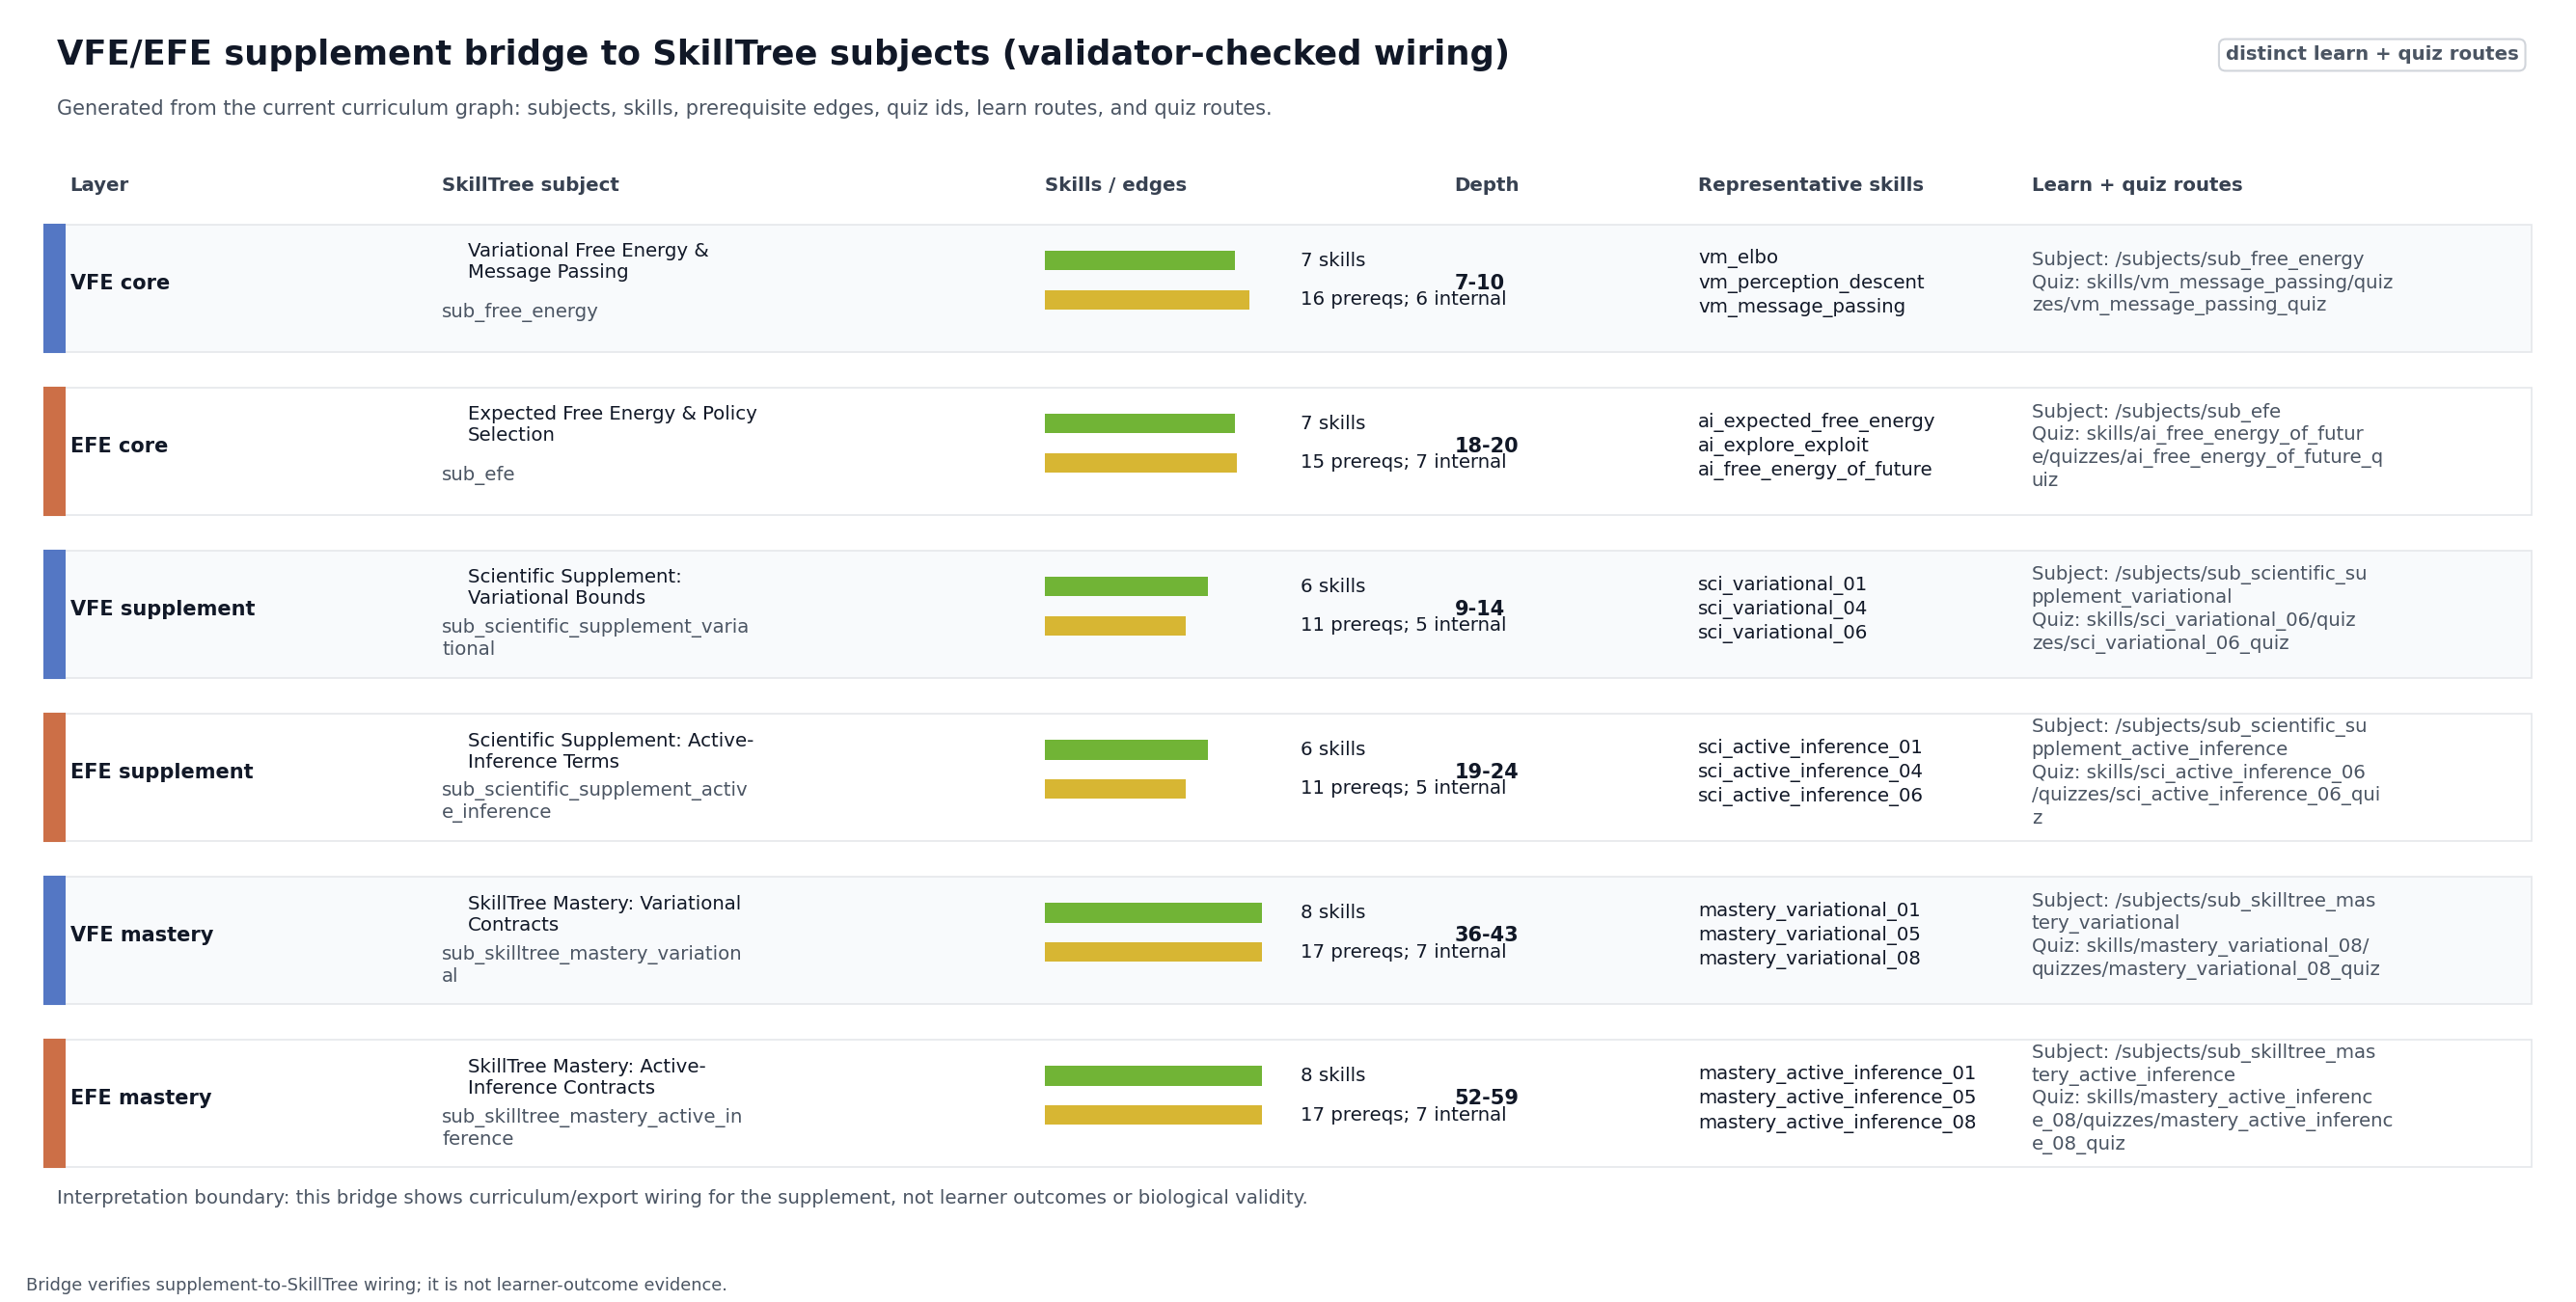
\includegraphics[width=1\linewidth,height=0.5\textheight,keepaspectratio,alt={VFE/EFE SkillTree bridge generated from the current curriculum graph after structural checks. Rows are real SkillTree subjects, columns report skill counts, prerequisite-edge counts, graph-depth ranges, representative skill IDs, and learn-route and quiz-route fragments that expose the subject identifiers; color marks separate VFE-centered rows from EFE-centered rows. The figure connects the supplement's mathematical plots to quiz-gated curriculum nodes and prevents the derivation from being presented as a standalone artifact disconnected from the learning path.}]{../figures/vfe_efe_skilltree_bridge.png}
\caption{VFE/EFE SkillTree bridge generated from the current curriculum
graph after structural checks. Rows are real SkillTree subjects, columns
report skill counts, prerequisite-edge counts, graph-depth ranges,
representative skill IDs, and learn-route and quiz-route fragments that
expose the subject identifiers; color marks separate VFE-centered rows
from EFE-centered rows. The figure connects the supplement's
mathematical plots to quiz-gated curriculum nodes and prevents the
derivation from being presented as a standalone artifact disconnected
from the learning path.}\label{fig:vfe_efe_skilltree_bridge}
\end{figure}

\subsection{Noisy-sensor posterior and the tight variational-free-energy
bound}\label{noisy-sensor-posterior-and-the-tight-variational-free-energy-bound}

On a noisy-sensor model with a \(1\%\) base rate, \(99\%\) sensitivity,
and \(95\%\) specificity, a positive observation yields a posterior of
0.166667 for the latent condition. This is the same base-rate
calibration problem that makes Bayesian reasoning difficult in
natural-language judgment tasks and motivates frequency-format teaching
examples for Bayesian inference
\citep{cosmides1996intuitive, gigerenzer1995bayesian}. The evidence
probability of the positive observation is 0.0594, so the observation
surprise is 2.82346 nats.

{\def\LTcaptype{none} % do not increment counter
\begin{longtable}[]{@{}
  >{\raggedright\arraybackslash}p{(\linewidth - 2\tabcolsep) * \real{0.5000}}
  >{\raggedright\arraybackslash}p{(\linewidth - 2\tabcolsep) * \real{0.5000}}@{}}
\toprule\noalign{}
\begin{minipage}[b]{\linewidth}\raggedright
Noisy-sensor parameter
\end{minipage} & \begin{minipage}[b]{\linewidth}\raggedright
Paper value
\end{minipage} \\
\midrule\noalign{}
\endhead
\bottomrule\noalign{}
\endlastfoot
Latent states & \texttt{present}, \texttt{absent} \\
Observation index & \texttt{positive} \\
Prior \(D\) & \([0.01, 0.99]\) \\
Likelihood rows \(A_{o,s}\) & \texttt{positive}: \([0.99, 0.05]\);
\texttt{negative}: \([0.01, 0.95]\) \\
VFE sweep coordinate & \(q(\mathrm{present})\) over \([0.001, 0.999]\),
plus the exact posterior and \(0.5\) \\
\end{longtable}
}

Evaluating variational free energy across beliefs confirms the central
inequality: a uniform belief gives 3.11735 nats, while the true
posterior gives 2.82346 nats, exactly the negative log-evidence.
fig.~\ref{fig:free_energy} shows the full one-dimensional sweep over
\(q(\mathrm{present})\): the curve bottoms out at the exact posterior
and stays above the surprise line everywhere else. The plot should not
be read as a universal geometry of all recognition densities. It is a
controlled diagnostic for one discrete model, one observation and one
belief coordinate.

\begin{figure}
\centering
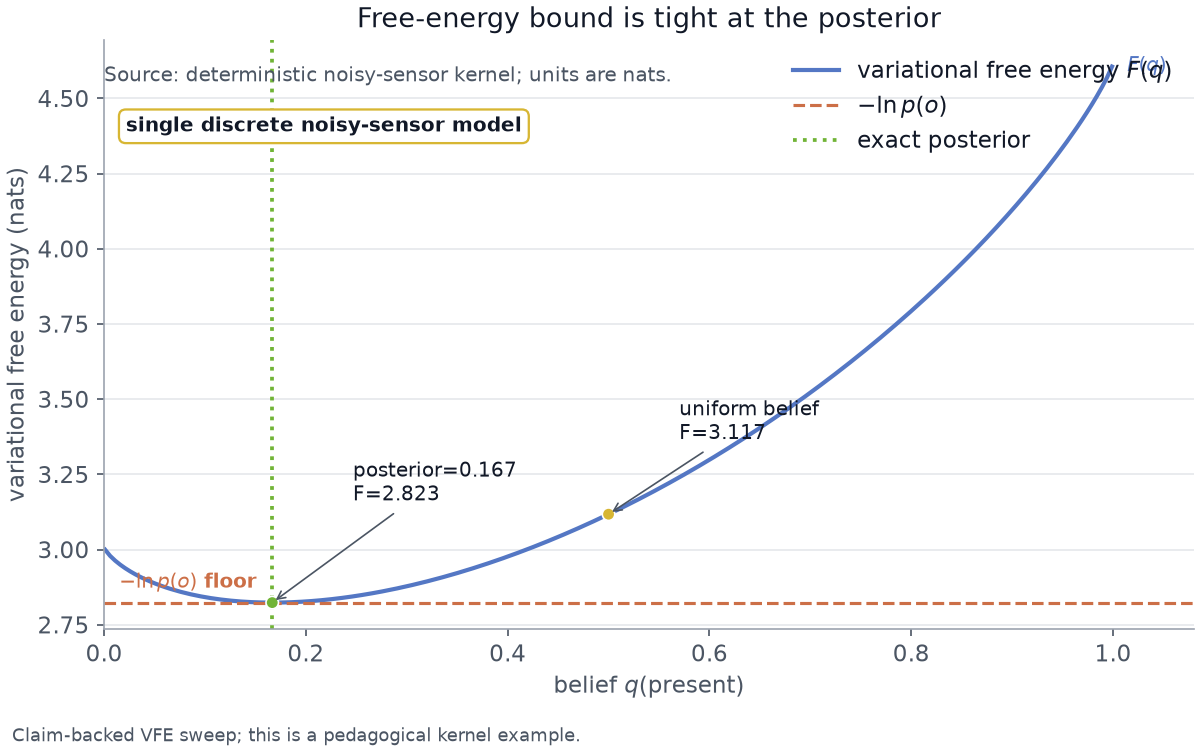
\includegraphics[width=1\linewidth,height=0.5\textheight,keepaspectratio,alt={Variational free-energy sweep for the noisy-sensor model, generated from the same claim-registry kernels that provide the manuscript tokens and taught through the VFE core, supplement, and mastery SkillTree subjects in the VFE/EFE SkillTree bridge. The x-axis is the recognition belief q(\textbackslash mathrm\{present\}), the blue curve is F(q) in nats, the horizontal dashed line is -\textbackslash ln p(o), the vertical dotted line is the exact posterior, and the labeled points compare the looser uniform belief with the posterior value. The intended takeaway is bound tightness at the posterior for this one discrete model and observation; the plot does not establish that the model is true or that the same geometry holds for every recognition family.}]{../figures/free_energy_descent.png}
\caption{Variational free-energy sweep for the noisy-sensor model,
generated from the same claim-registry kernels that provide the
manuscript tokens and taught through the VFE core, supplement, and
mastery SkillTree subjects in the VFE/EFE SkillTree bridge. The x-axis
is the recognition belief \(q(\mathrm{present})\), the blue curve is
\(F(q)\) in nats, the horizontal dashed line is \(-\ln p(o)\), the
vertical dotted line is the exact posterior, and the labeled points
compare the looser uniform belief with the posterior value. The intended
takeaway is bound tightness at the posterior for this one discrete model
and observation; the plot does not establish that the model is true or
that the same geometry holds for every recognition
family.}\label{fig:free_energy}
\end{figure}

\subsection{Expected free energy: epistemic value and bounded policy
comparison}\label{expected-free-energy-epistemic-value-and-bounded-policy-comparison}

Decomposing expected free energy on an informative sensor shows that an
uncertain belief carries positive epistemic value (0.368064 nats) while
a certain belief carries none (0 nats): once the state is known, an
observation cannot reduce uncertainty. In the two-action agent,
preferences are neutral, so the pragmatic term is identical for both
actions and the choice is decided by information gain. Under the
lower-is-better \(G(\pi)\) convention above, the information-seeking
\emph{sample} action scores lower expected free energy (0.546837 nats)
than \emph{commit} (0.613267 nats), because it carries higher epistemic
value (0.146311 nats versus 0.079881 nats). This is the epistemic drive
of Active Inference: no separate curiosity bonus is required in the
reference formulation used here
\citep{friston2015epistemic, friston2017curiosity, dacosta2020synthesis, sajid2021demystified}.
Derivation and unification work is the reason the supplement keeps the
formulation explicit instead of presenting ``expected free energy'' as a
single unqualified object
\citep{millidge2021whence, champion2026reframing, nuijten2026what_type_inference, nuijten2026efe_planning_vi}.

\subsubsection{Preference convention and
parameters}\label{preference-convention-and-parameters}

One convention should be made explicit here: the kernel normalizes the
preference vector \(C\) to a probability distribution before taking its
logarithm for the pragmatic term (\breaktt{preferences\ =\ normalize(C)},
then \(\mathbb{E}_{q(o)}[\ln \mathrm{normalize}(C)]\)), so the values
plotted above assume \(C\) is a preference \emph{distribution}. This is
a specific modeling choice rather than the only option: canonical Active
Inference often treats \(C\) directly as a vector of log-preferences,
which shifts the pragmatic term by an additive constant and can change
its scale relative to the epistemic term.

\subsubsection{EFE parameter table}\label{efe-parameter-table}

{\def\LTcaptype{none} % do not increment counter
\begin{longtable}[]{@{}
  >{\raggedright\arraybackslash}p{(\linewidth - 2\tabcolsep) * \real{0.5000}}
  >{\raggedright\arraybackslash}p{(\linewidth - 2\tabcolsep) * \real{0.5000}}@{}}
\toprule\noalign{}
\begin{minipage}[b]{\linewidth}\raggedright
EFE sample/commit parameter
\end{minipage} & \begin{minipage}[b]{\linewidth}\raggedright
Paper value
\end{minipage} \\
\midrule\noalign{}
\endhead
\bottomrule\noalign{}
\endlastfoot
Sensor likelihood & \(A=[[p,1-p],[1-p,p]]\), with \(p=0.9\) \\
EFE decomposition preference & \(C=[0.9,0.1]\) for the
informative-sensor term example \\
Agent preference & Neutral \(C=[0.5,0.5]\) for the sample/commit policy
comparison \\
Prior before observation & \(D=[0.5,0.5]\) \\
Actions & \texttt{sample} uses identity dynamics; \texttt{commit} maps
both prior states toward state \texttt{0} with transition columns
\([0.95,0.05]\) \\
Policy posterior & \(q(\pi)=\mathrm{softmax}(-\gamma G_\pi)\) over the
two one-step policies \\
\end{longtable}
}

\subsection{Sensor precision as a sample-versus-commit policy
boundary}\label{sensor-precision-as-a-sample-versus-commit-policy-boundary}

The expected-free-energy result is not a universal law. It is pinned to
a specific moderate-precision regime: at sensor precision \(0.9\),
sampling wins; at the computed switch precision 0.95, sample and commit
tie; above that point, the commit action can become lower in expected
free energy. fig.~\ref{fig:efe} shows both the sample/commit comparison
and the precision sweep, making the regime boundary explicit instead of
hiding it in prose
\citep{millidge2021whence, champion2026reframing, nuijten2026what_type_inference, nuijten2026efe_planning_vi}.

{\def\LTcaptype{none} % do not increment counter
\begin{longtable}[]{@{}
  >{\raggedright\arraybackslash}p{(\linewidth - 2\tabcolsep) * \real{0.5000}}
  >{\raggedright\arraybackslash}p{(\linewidth - 2\tabcolsep) * \real{0.5000}}@{}}
\toprule\noalign{}
\begin{minipage}[b]{\linewidth}\raggedright
Precision-sweep parameter
\end{minipage} & \begin{minipage}[b]{\linewidth}\raggedright
Paper value
\end{minipage} \\
\midrule\noalign{}
\endhead
\bottomrule\noalign{}
\endlastfoot
Sensor precision range & \(p \in [0.5,0.99]\) with the computed switch
inserted into the grid \\
Sweep samples & \(101\) grid samples before inserting \(p=0.9\) and the
switch precision \\
Prior, preference, actions & Same neutral two-action agent as the
sample/commit comparison \\
Tie criterion & The switch is the bisection point where
\(G_{\mathrm{sample}}-G_{\mathrm{commit}}=0\) \\
\end{longtable}
}

\begin{figure}
\centering
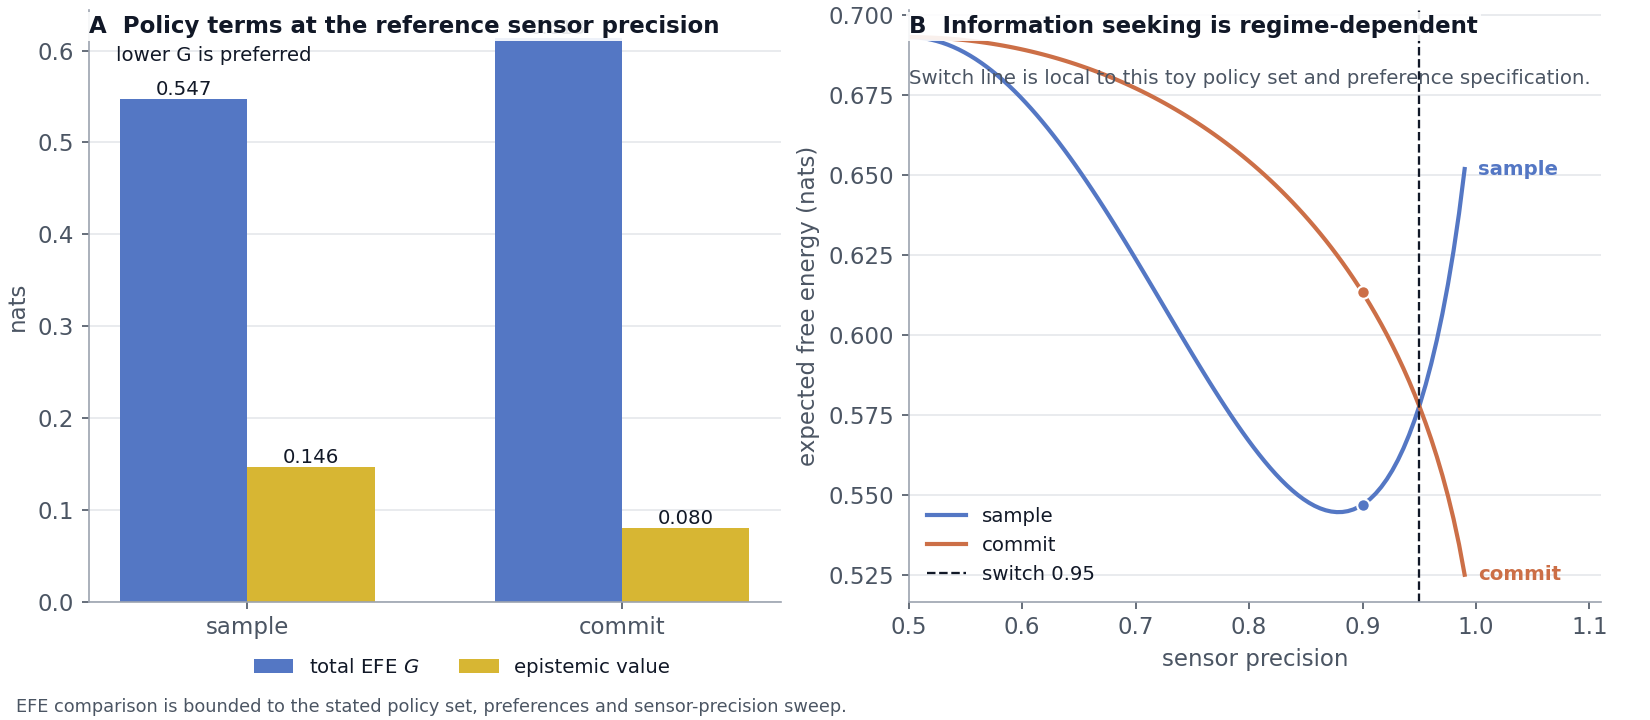
\includegraphics[width=1\linewidth,height=0.5\textheight,keepaspectratio,alt={Expected free-energy decomposition for the sample/commit task, generated from the discrete active-inference kernel and taught through the EFE core, supplement, and mastery SkillTree subjects in the VFE/EFE SkillTree bridge. The left panel compares total expected free energy and epistemic value for the two policies at sensor precision 0.9; the right panel sweeps sensor precision and marks the computed sample/commit switch. The visual encoding keeps policy score and epistemic value separate so the reader can see why sampling is preferred in the reference regime, while the right panel prevents the teaching example from being overgeneralized beyond the stated policy set and preferences.}]{../figures/efe_decomposition.png}
\caption{Expected free-energy decomposition for the sample/commit task,
generated from the discrete active-inference kernel and taught through
the EFE core, supplement, and mastery SkillTree subjects in the VFE/EFE
SkillTree bridge. The left panel compares total expected free energy and
epistemic value for the two policies at sensor precision \(0.9\); the
right panel sweeps sensor precision and marks the computed sample/commit
switch. The visual encoding keeps policy score and epistemic value
separate so the reader can see why sampling is preferred in the
reference regime, while the right panel prevents the teaching example
from being overgeneralized beyond the stated policy set and
preferences.}\label{fig:efe}
\end{figure}

fig.~\ref{fig:kernel_sensitivity_profiles} broadens the sensitivity view
without changing the evidence class. The left panel varies the base rate
in the same noisy-sensor likelihood and shows how a positive
observation's posterior changes as the prior changes. The middle panel
repeats the VFE bound profile so the equality point remains tied to the
exact posterior. The right panel repeats the EFE precision sweep and
marks the computed sample/commit boundary. These panels are
deterministic kernel diagnostics: they identify where the teaching
example is stable or regime-limited, not whether a learner or a
biological system will behave that way.

\begin{figure}
\centering
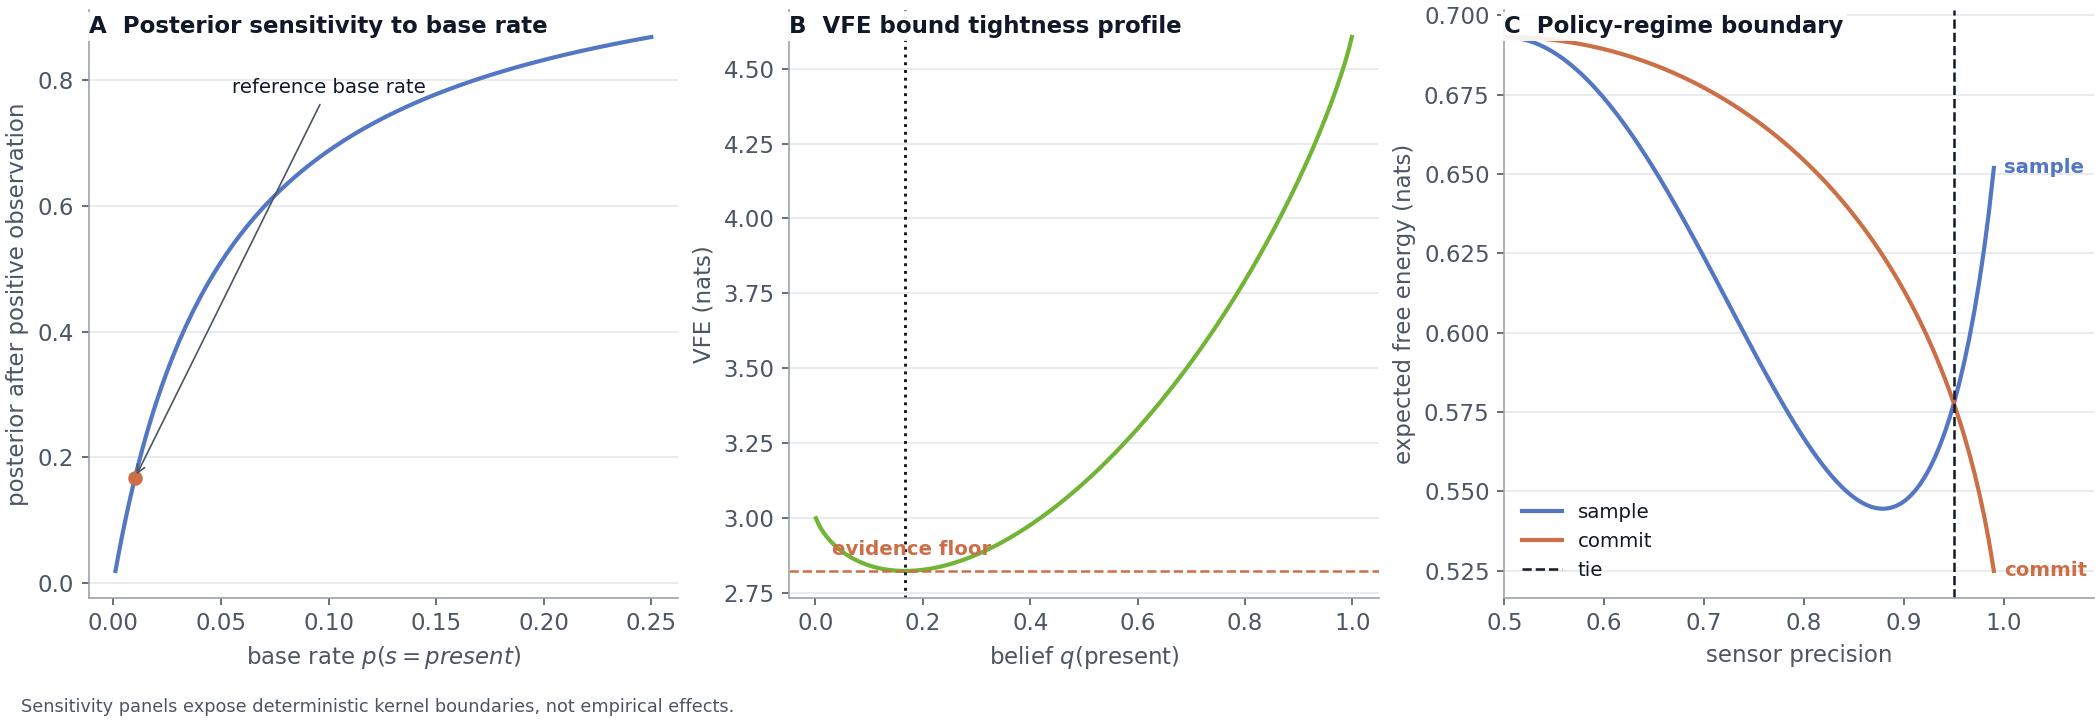
\includegraphics[width=1\linewidth,height=0.5\textheight,keepaspectratio,alt={Kernel sensitivity profiles for the supplemental examples, generated from the noisy-sensor posterior, VFE sweep, and EFE precision sweep, then positioned in the SkillTree bridge as a route from mathematical identity to quiz-gated interpretation. The left panel varies the base rate and shows posterior sensitivity after a positive observation, the middle panel plots the VFE bound profile with posterior and evidence references, and the right panel sweeps expected free energy for sample and commit policies across sensor precision while marking the computed policy switch. These panels identify deterministic regime boundaries for teaching examples; they are not empirical estimates, confidence intervals, or learner outcome statistics.}]{../figures/kernel_sensitivity_profiles.png}
\caption{Kernel sensitivity profiles for the supplemental examples,
generated from the noisy-sensor posterior, VFE sweep, and EFE precision
sweep, then positioned in the SkillTree bridge as a route from
mathematical identity to quiz-gated interpretation. The left panel
varies the base rate and shows posterior sensitivity after a positive
observation, the middle panel plots the VFE bound profile with posterior
and evidence references, and the right panel sweeps expected free energy
for sample and commit policies across sensor precision while marking the
computed policy switch. These panels identify deterministic regime
boundaries for teaching examples; they are not empirical estimates,
confidence intervals, or learner outcome
statistics.}\label{fig:kernel_sensitivity_profiles}
\end{figure}

\subsection{Exact inference on a chain with sum-product belief
propagation}\label{exact-inference-on-a-chain-with-sum-product-belief-propagation}

The message-passing curriculum is bound to a worked example rather than
left as prose. Because the example factor graph is acyclic, sum-product
belief propagation returns the exact node marginals for a three-node
sticky latent chain with a single informative reading at the middle
node. The observed node settles at 0.9, and the smoothing message lifts
each unobserved neighbor from its prior to 0.74 -- a lift of 0.24 that
is produced purely by propagating the one reading along the transition
factor. Because a chain is a tree, these marginals are the same numbers
a brute-force enumeration of the full joint would give; the test suite
pins that equality, so the example is an exact-inference check, not an
approximation
\citep{kschischang2001factor_graphs, pearl1988probabilistic_reasoning, parr2022active}.
Factor-graph message passing is also a live implementation path for EFE
minimization, but this supplement uses the chain only to teach exact
sum-product inference and keeps policy-optimization message passing out
of scope for this release \citep{nuijten2025message_passing_efe}.

\subsubsection{Sum-product parameter
table}\label{sum-product-parameter-table}

{\def\LTcaptype{none} % do not increment counter
\begin{longtable}[]{@{}
  >{\raggedright\arraybackslash}p{(\linewidth - 2\tabcolsep) * \real{0.5000}}
  >{\raggedright\arraybackslash}p{(\linewidth - 2\tabcolsep) * \real{0.5000}}@{}}
\toprule\noalign{}
\begin{minipage}[b]{\linewidth}\raggedright
Sum-product parameter
\end{minipage} & \begin{minipage}[b]{\linewidth}\raggedright
Paper value
\end{minipage} \\
\midrule\noalign{}
\endhead
\bottomrule\noalign{}
\endlastfoot
Chain length & \(3\) binary latent nodes \\
Prior on node \(0\) & \([0.5,0.5]\) \\
Sticky transition & \([[0.8,0.2],[0.2,0.8]]\) \\
Evidence potentials & node \(0\): \([1,1]\); node \(1\): \([0.9,0.1]\);
node \(2\): \([1,1]\) \\
\end{longtable}
}

\subsection{Conjugate parameter learning from Dirichlet
beliefs}\label{conjugate-parameter-learning-from-dirichlet-beliefs}

Parameter learning is shown as a Dirichlet-conjugate update of one
sensor column. A flat prior has mean 0.5; after a fixed observed count
vector the posterior mean sharpens to 0.75, and the expected
log-parameter that variational message passing actually consumes is
-0.30202 nats, computed through the digamma identity
\(\mathbb{E}[\ln p_i]=\psi(\alpha_i)-\psi(\sum_j\alpha_j)\). This is the
learning half of active inference: beliefs about model parameters move
with evidence, not just beliefs about states
\citep{dacosta2020synthesis}.

\subsection{Bayesian model reduction: whether data require added
structure}\label{bayesian-model-reduction-whether-data-require-added-structure}

Bayesian model reduction compares the evidence of a full model against a
reduced model whose pruned state carries negligible prior mass. After a
positive reading on the noisy-sensor model the full-model log evidence
is -2.82346 nats and the reduced-model log evidence is -2.99571 nats, so
the log Bayes factor is 0.172252 nats. The positive sign says the data
support keeping the pruned structure: the reduced model is rejected.
Both terms are exact log evidences, so the reported factor is the
difference of two computed numbers rather than a hand-typed value
\citep{friston2018bayesian_model_reduction, parr2022active}.

{\def\LTcaptype{none} % do not increment counter
\begin{longtable}[]{@{}
  >{\raggedright\arraybackslash}p{(\linewidth - 2\tabcolsep) * \real{0.5000}}
  >{\raggedright\arraybackslash}p{(\linewidth - 2\tabcolsep) * \real{0.5000}}@{}}
\toprule\noalign{}
\begin{minipage}[b]{\linewidth}\raggedright
BMR parameter
\end{minipage} & \begin{minipage}[b]{\linewidth}\raggedright
Paper value
\end{minipage} \\
\midrule\noalign{}
\endhead
\bottomrule\noalign{}
\endlastfoot
Full prior & \(D=[0.01, 0.99]\) \\
Reduced prior & the \texttt{present} state is set to \(10^{-6}\) and the
prior vector is renormalized \\
Observation and likelihood & same positive observation and noisy-sensor
likelihood as the VFE example \\
Score & \(\log P(o\mid\mathrm{full})-\log P(o\mid\mathrm{reduced})\) \\
\end{longtable}
}

\subsection{Ambiguity as a state-dependent component of expected free
energy}\label{ambiguity-as-a-state-dependent-component-of-expected-free-energy}

Expected free energy carries an ambiguity term -- the expected entropy
of the likelihood columns -- that the main decomposition leaves
implicit. On an asymmetric sensor whose two states differ in how noisy
their readings are, the crisp state has likelihood entropy 0.325083
nats, while a uniform belief averages to 0.509115 nats. Ambiguity is
therefore a property of where the agent believes it is, which is why
reducing it is part of what drives exploration
\citep{parr2022active, sajid2021demystified}.

\subsection{Multi-step planning and model-dependent look-ahead
value}\label{multi-step-planning-and-model-dependent-look-ahead-value}

The one-step agent above is generalized to a planner that scores every
length-\(H\) action sequence by its cumulative expected free energy and
forms a posterior over policies,
\(q(\pi)=\mathrm{softmax}(-\gamma G_\pi)\); at \(H=1\) the per-policy
values reduce exactly to the one-step result, a consistency invariant
the tests pin. Whether planning beats a myopic agent is then a measured
question, not an assumption, and the answer is regime dependent.

In a decoupled sample/commit model the optimal multi-step plan coincides
with the strongest greedy policy, so the look-ahead gain is exactly 0
nats -- an honest null. In a coupled investment model, where a state
that is myopically attractive blocks access to a higher-value goal, the
planner pays a worse first step to reach the goal: the greedy policy
scores 3.02826 nats, the optimal plan scores 2.20728 nats, and the
look-ahead gain is 0.820981 nats with the policy posterior concentrating
0.915376 of its mass on the winning plan
(fig.~\ref{fig:planning_lookahead}). The comparator is the strongest
myopic policy, not a weakened straw baseline, so the gain is a fair
number; the first-principles lesson is that look-ahead pays only when
immediate and long-run value diverge
\citep{parr2022active, dacosta2020synthesis}.

{\def\LTcaptype{none} % do not increment counter
\begin{longtable}[]{@{}
  >{\raggedright\arraybackslash}p{(\linewidth - 4\tabcolsep) * \real{0.3333}}
  >{\raggedright\arraybackslash}p{(\linewidth - 4\tabcolsep) * \real{0.3333}}
  >{\raggedright\arraybackslash}p{(\linewidth - 4\tabcolsep) * \real{0.3333}}@{}}
\toprule\noalign{}
\begin{minipage}[b]{\linewidth}\raggedright
Planning parameter
\end{minipage} & \begin{minipage}[b]{\linewidth}\raggedright
Decoupled sample/commit model
\end{minipage} & \begin{minipage}[b]{\linewidth}\raggedright
Coupled investment model
\end{minipage} \\
\midrule\noalign{}
\endhead
\bottomrule\noalign{}
\endlastfoot
States & \(2\) latent states & \texttt{start}, \texttt{comfort},
\texttt{goal}, \texttt{climb} \\
Observation model & informative sensor with \(p=0.9\) & identity
likelihood \\
Preference vector & \(C=[0.9,0.1]\) & \(C=[0.03,0.22,0.55,0.20]\) \\
Initial prior & \(D=[0.5,0.5]\) & \(D=[1,0,0,0]\) \\
Actions & \texttt{sample} identity; \texttt{commit} collapse toward
state \texttt{0} & \texttt{comfort} sends start to comfort;
\texttt{climb} sends start to climb and climb to goal \\
Horizon and policy precision & \(H=2\), \(\gamma=4\) & \(H=2\),
\(\gamma=4\) \\
\end{longtable}
}

\begin{figure}
\centering
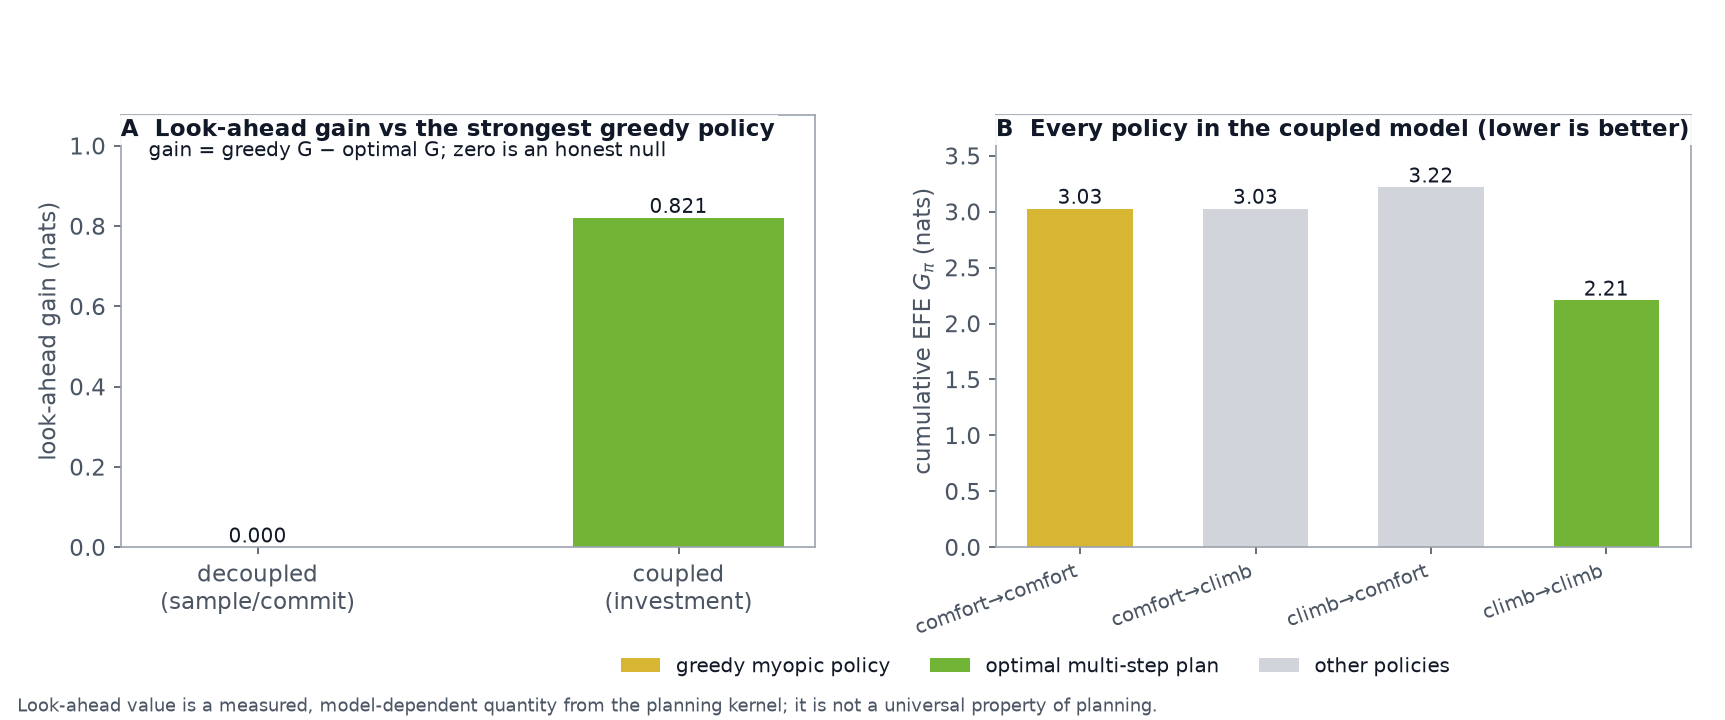
\includegraphics[width=1\linewidth,height=0.5\textheight,keepaspectratio,alt={Multi-step planning look-ahead, generated from the discrete active-inference planning kernel. The left panel contrasts the measured look-ahead gain (optimal multi-step plan versus the strongest greedy myopic policy) in a decoupled model, where the gain is zero, and a coupled investment model, where paying a worse first step to unlock the goal yields a positive gain. The right panel shows the cumulative expected free energy of every enumerated policy in the coupled model, with the greedy and optimal policies marked. The panel demonstrates that look-ahead value is a measured, model-dependent quantity, not a universal property of planning.}]{../figures/planning_lookahead.png}
\caption{Multi-step planning look-ahead, generated from the discrete
active-inference planning kernel. The left panel contrasts the measured
look-ahead gain (optimal multi-step plan versus the strongest greedy
myopic policy) in a decoupled model, where the gain is zero, and a
coupled investment model, where paying a worse first step to unlock the
goal yields a positive gain. The right panel shows the cumulative
expected free energy of every enumerated policy in the coupled model,
with the greedy and optimal policies marked. The panel demonstrates that
look-ahead value is a measured, model-dependent quantity, not a
universal property of planning.}\label{fig:planning_lookahead}
\end{figure}

\subsection{Continuous predictive coding as model-specific
prediction-error
descent}\label{continuous-predictive-coding-as-model-specific-prediction-error-descent}

The discrete examples above update beliefs in one shot; the
continuous-state face of the Free Energy Principle instead
\emph{settles} a latent estimate by descending the free energy along
precision-weighted prediction errors. On a single linear-Gaussian level
-- a vague unit-variance prior at zero meeting a more precise reading of
2 -- the estimate relaxes from the prior mean to 1.33333, the exact
analytic posterior mean, where the sensory prediction error (0.666667)
and the prior prediction error (1.33333) balance once each is weighted
by its precision.

fig.~\ref{fig:predictive_coding} shows the estimate converging to that
fixed point while, under the stated objective and step size used in this
simulation, the free energy decreases monotonically to its analytic
minimum. The result is exact for the linear-Gaussian case the kernel
tests pin against a closed form; it is a controlled teaching example,
not a claim that prediction-error descent is exact for nonlinear or
hierarchical models
\citep{kalman1960linear_filtering, sarkka2013bayesian, buckley2017free, parr2022active, kataoka2026extended_predictive_coding}.

{\def\LTcaptype{none} % do not increment counter
\begin{longtable}[]{@{}
  >{\raggedright\arraybackslash}p{(\linewidth - 2\tabcolsep) * \real{0.5000}}
  >{\raggedright\arraybackslash}p{(\linewidth - 2\tabcolsep) * \real{0.5000}}@{}}
\toprule\noalign{}
\begin{minipage}[b]{\linewidth}\raggedright
Predictive-coding parameter
\end{minipage} & \begin{minipage}[b]{\linewidth}\raggedright
Paper value
\end{minipage} \\
\midrule\noalign{}
\endhead
\bottomrule\noalign{}
\endlastfoot
Prior mean and variance & \(\mu_0=0\), \(\sigma_0^2=1\) \\
Observation and variance & \(y=2\), \(\sigma_y^2=0.5\) \\
Descent rate and steps & rate \(0.1\), maximum \(400\) steps \\
Analytic target & Gaussian posterior mean from the linear filtering
update \\
\end{longtable}
}

\begin{figure}
\centering
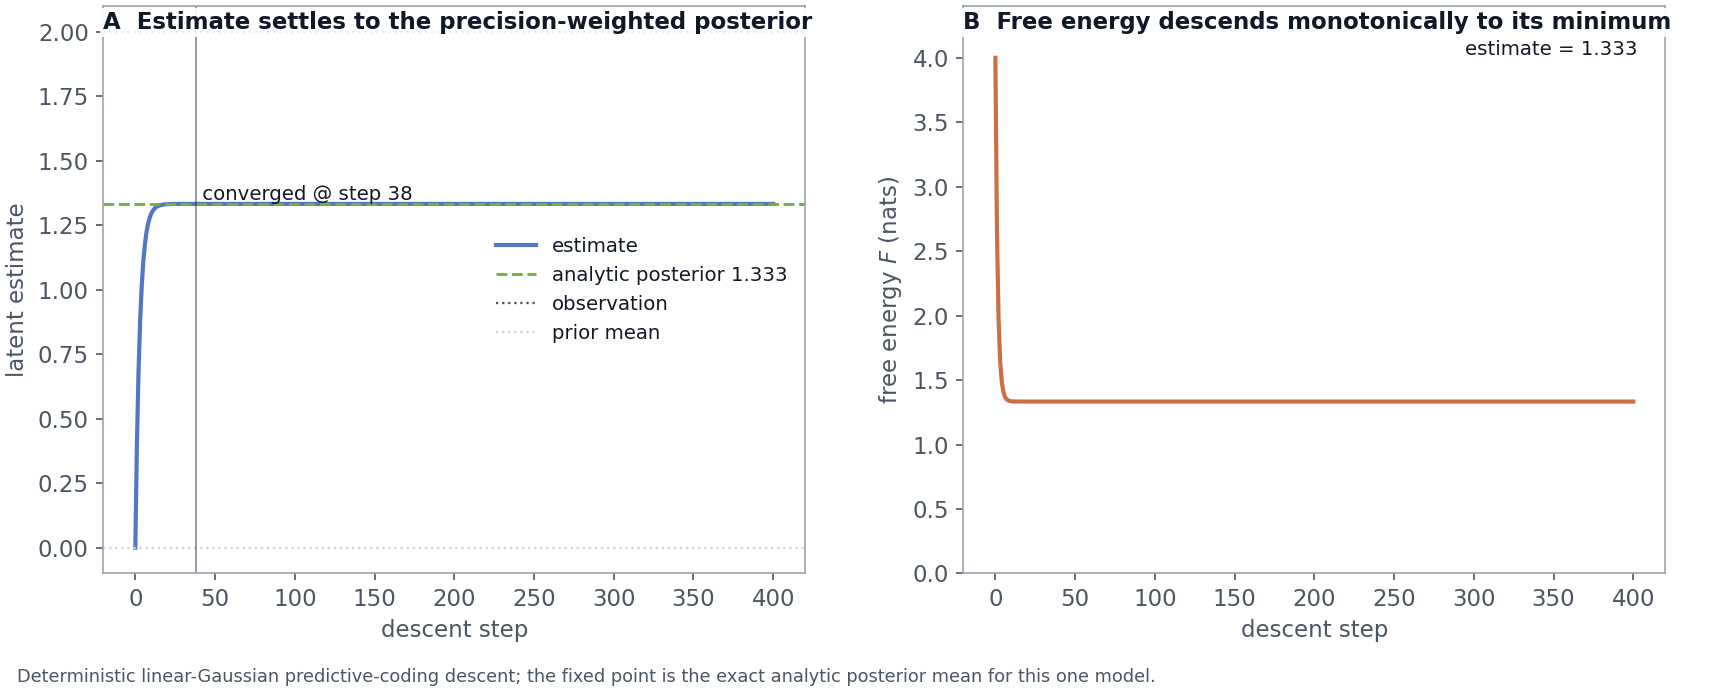
\includegraphics[width=1\linewidth,height=0.5\textheight,keepaspectratio,alt={Continuous predictive-coding descent generated from the linear-Gaussian kernel. The left panel traces the latent estimate from the prior mean to the analytic precision-weighted posterior (dashed) as it balances the sensory and prior prediction errors; the right panel shows the free energy descending monotonically to its analytic minimum. The figure supports a bounded claim that prediction-error descent implements exact Gaussian inference for this one model, not a universal convergence guarantee for all generative models.}]{../figures/predictive_coding_descent.png}
\caption{Continuous predictive-coding descent generated from the
linear-Gaussian kernel. The left panel traces the latent estimate from
the prior mean to the analytic precision-weighted posterior (dashed) as
it balances the sensory and prior prediction errors; the right panel
shows the free energy descending monotonically to its analytic minimum.
The figure supports a bounded claim that prediction-error descent
implements exact Gaussian inference for this one model, not a universal
convergence guarantee for all generative
models.}\label{fig:predictive_coding}
\end{figure}

\newpage

\section{Code and Data
Availability}\label{sec:code-and-data-availability}

The artifact described here is a single repository containing the
kernels, the curriculum catalog, the SkillTree exporter, the learner
dashboard, the manuscript sources, and every validator named in
sec.~\ref{sec:reproducibility}. Authored code and content are MIT
licensed with Daniel Ari Friedman as the copyright holder, recorded in
\texttt{LICENSE} and mirrored in the citation, CodeMeta, and Zenodo
metadata files. Vendored runtime dependencies and their separate notices
are listed in \breaktt{THIRD\_PARTY\_NOTICES.md}. External Active
Inference Institute course and knowledge-base material is referenced by
repository, path, and commit rather than copied, so upstream licensing
stays with upstream.

The code is public at
\href{https://github.com/ActiveInferenceInstitute/Active_Skillference}{github.com/ActiveInferenceInstitute/Active\_Skillference},
with the v1.0.0 manuscript archived on Zenodo at
\href{https://doi.org/10.5281/zenodo.21865644}{doi.org/10.5281/zenodo.21865644}.
The identifier appears on the cover page, in the citation file, in the
CodeMeta and Zenodo records, and in the archived copy of this document,
all naming the same deposit. That agreement is enforced rather than
assumed: a test cross-checks each surface against the recorded deposit
and fails on any divergence, which is what keeps a plausible but wrong
identifier out of a citation. Version-specific identifiers stay blank
because no versioned deposit beyond this one exists, and the same test
holds them blank.

Generated outputs travel with the repository even though they are
rebuildable, so a reader can open the manuscript, the figures, the
SkillTree export, and every audit record without installing anything or
running the pipeline. Committing them does not soften the regenerability
claim: running the kernels rebuilds the claim ledger, manuscript
variables, scholarship audits, figures, lesson records, and the export
from source, and the freshness validator fails if a committed artifact
has drifted from what the current source produces. Only build detritus
is withheld, meaning renderer logs and intermediates that change on
every run and carry nothing a reader would read. The captured evidence
described in sec.~\ref{sec:results-skilltree-dashboard-front-matter} is
different in kind rather than in handling: a recording of a running
system is not a function of project data and cannot be rebuilt from a
checkout at all, which is why it is stored beside a provenance record
naming the dashboard address, viewport, live counts, full-stack mode,
capture timestamp, and a digest per image. Every other image in this
paper regenerates; those five are archived precisely because they do
not.

\newpage

\section{References: Bibliography and Source-Role
Audit}\label{sec:references}

Bibliography lives in
\href{references.bib}{\breaktt{manuscript/references.bib}} and is read by
Pandoc during PDF render. The build pipeline invokes Pandoc with
\texttt{-\/-natbib}, so every \texttt{{[}@key{]}} citation in the
manuscript is rewritten to the appropriate
\texttt{\textbackslash{}cite\{\}}/\texttt{\textbackslash{}citep\{\}}/\texttt{\textbackslash{}citet\{\}}
LaTeX command and resolved against the bib file.

To validate that \texttt{references.bib} is syntactically clean and
contains the required fields per entry type:

\begin{Shaded}
\begin{Highlighting}[]
\ExtensionTok{uv}\NormalTok{ run python }\AttributeTok{{-}m}\NormalTok{ infrastructure.reference.citation.cli validate }\DataTypeTok{\textbackslash{}}
\NormalTok{    manuscript/references.bib }\AttributeTok{{-}{-}strict}
\end{Highlighting}
\end{Shaded}




\providecommand{\bibsection}{}
\renewcommand{\bibsection}{}

\bibliography{references}
\end{document}
